\documentclass[12pt, twoside, openright]{report} %fuente a 12pt, formato doble pagina y chapter a la derecha
\raggedbottom % No ajustar el contenido con un salto de pagina

% MÁRGENES: 2,5 cm sup. e inf.; 3 cm izdo. y dcho.
\usepackage[
a4paper,
vmargin=2.5cm,
hmargin=3cm
]{geometry}

% INTERLINEADO: Estrecho (6 ptos./interlineado 1,15) o Moderado (6 ptos./interlineado 1,5)
\renewcommand{\baselinestretch}{1.15}
\parskip=6pt

% DEFINICIÓN DE COLORES para portada y listados de código
\usepackage[table]{xcolor}
\definecolor{azulUC3M}{RGB}{0,0,102}
\definecolor{gray97}{gray}{.97}
\definecolor{gray75}{gray}{.75}
\definecolor{gray45}{gray}{.45}

% Soporte para GENERAR PDF/A
\usepackage[a-1b]{pdfx}

% ENLACES
\usepackage{hyperref}
\hypersetup{colorlinks=true,
	linkcolor=black, % enlaces a partes del documento (p.e. índice) en color negro
	urlcolor=blue} % enlaces a recursos fuera del documento en azul

% Añadir pdfs como partes del documento
\usepackage{pdfpages}

% Quitar la indentación de principio de los parrafos
\setlength{\parindent}{0em}

% EXPRESIONES MATEMATICAS
\usepackage{amsmath,amssymb,amsfonts,amsthm}

\usepackage{txfonts} 
\usepackage[T1]{fontenc}
\usepackage[utf8]{inputenc}

% Insertar graficas y fotos
\usepackage{tikz}
\usepackage{pgfplots}

\usepackage[spanish, es-tabla]{babel} 
\usepackage[babel, spanish=spanish]{csquotes}
\AtBeginEnvironment{quote}{\small}

% diseño de PIE DE PÁGINA
\usepackage{fancyhdr}
\pagestyle{fancy}
\fancyhf{}
\renewcommand{\headrulewidth}{0pt}
\fancyfoot[LE,RO]{\thepage}
\fancypagestyle{plain}{\pagestyle{fancy}}

% DISEÑO DE LOS TÍTULOS de las partes del trabajo (capítulos y epígrafes o subcapítulos)
\usepackage{titlesec}
\usepackage{titletoc}
\titleformat{\chapter}[block]
{\large\bfseries\filcenter}
{\thechapter.}
{5pt}
{\MakeUppercase}
{}
\titlespacing{\chapter}{0pt}{0pt}{*3}
\titlecontents{chapter}
[0pt]                                               
{}
{\contentsmargin{0pt}\thecontentslabel.\enspace\uppercase}
{\contentsmargin{0pt}\uppercase}                        
{\titlerule*[.7pc]{.}\contentspage}                 

\titleformat{\section}
{\bfseries}
{\thesection.}
{5pt}
{}
\titlecontents{section}
[5pt]                                               
{}
{\contentsmargin{0pt}\thecontentslabel.\enspace}
{\contentsmargin{0pt}}
{\titlerule*[.7pc]{.}\contentspage}

\titleformat{\subsection}
{\normalsize\bfseries}
{\thesubsection.}
{5pt}
{}
\titlecontents{subsection}
[10pt]                                               
{}
{\contentsmargin{0pt}                          
	\thecontentslabel.\enspace}
{\contentsmargin{0pt}}                        
{\titlerule*[.7pc]{.}\contentspage}  


% DISEÑO DE TABLAS.
\usepackage{multirow} % permite combinar celdas 
\usepackage{caption} % para personalizar el título de tablas y figuras
\usepackage{floatrow} % utilizamos este paquete y sus macros \ttabbox y \ffigbox para alinear los nombres de tablas y figuras de acuerdo con el estilo definido. Para su uso ver archivo de ejemplo 
\usepackage{array} % con este paquete podemos definir en la siguiente línea un nuevo tipo de columna para tablas: ancho personalizado y contenido centrado
\newcolumntype{P}[1]{>{\centering\arraybackslash}p{#1}}
\DeclareCaptionFormat{upper}{#1#2\uppercase{#3}\par}

% Diseño de tabla para ingeniería
\captionsetup[table]{
	format=hang,
	name=Tabla,
	justification=centering,
	labelsep=colon,
	width=.75\linewidth,
	labelfont=small,
	font=small,
}

% DISEÑO DE FIGURAS.
\usepackage{graphicx}
\graphicspath{{img/}} %ruta a la carpeta de imágenes

% Diseño de figuras para ingeniería
\captionsetup[figure]{
	format=hang,
	name=Fig.,
	singlelinecheck=off,
	labelsep=colon,
	labelfont=small,
	font=small		
}

% NOTAS A PIE DE PÁGINA
\usepackage{chngcntr} %para numeración continua de las notas al pie
\counterwithout{footnote}{chapter}

% LISTADOS DE CÓDIGO
% soporte y estilo para listados de código. Más información en https://es.wikibooks.org/wiki/Manual_de_LaTeX/Listados_de_código/Listados_con_listings
\usepackage{listings}

% definimos un estilo de listings
\lstdefinestyle{estilo}{ frame=Ltb,
	framerule=0pt,
	aboveskip=0.5cm,
	framextopmargin=3pt,
	framexbottommargin=3pt,
	framexleftmargin=0.4cm,
	framesep=0pt,
	rulesep=.4pt,
	backgroundcolor=\color{gray97},
	rulesepcolor=\color{black},
	%
	basicstyle=\ttfamily\footnotesize,
	keywordstyle=\bfseries,
	stringstyle=\ttfamily,
	showstringspaces = false,
	commentstyle=\color{gray45},     
	%
	numbers=left,
	numbersep=15pt,
	numberstyle=\tiny,
	numberfirstline = false,
	breaklines=true,
	xleftmargin=\parindent
}

\captionsetup[lstlisting]{font=small, labelsep=period}
% fijamos el estilo a utilizar 
\lstset{style=estilo}
\renewcommand{\lstlistingname}{\uppercase{Código}}

\pgfplotsset{compat=1.17} 
%-------------
%	DOCUMENTO
%-------------

\begin{document}
\pagenumbering{roman} % Se utilizan cifras romanas en la numeración de las páginas previas al cuerpo del trabajo
	
%----------
%	PORTADA
%----------	
\begin{titlepage}
	\begin{sffamily}
	\color{azulUC3M}
	\begin{center}
		\begin{figure}[H] %incluimos el logotipo de la Universidad
			\makebox[\textwidth][c]{
\includegraphics[width=16cm]{Portada_Logo.png}}
		\end{figure}
		\vspace{2.5cm}
		\begin{Large}
			Grado en Ingeniería Informática\\			
			2020-2021\\
			\vspace{2cm}		
			\textsl{Apuntes}\\
			\bigskip
		\end{Large}
		 	{\Huge Redes de ordenadores}\\
		 	\vspace*{0.5cm}
	 		\rule{10.5cm}{0.1mm}\\
			\vspace*{0.9cm}
			{\LARGE Jorge Rodríguez Fraile\footnote{\href{mailto:100405951@alumnos.uc3m.es}{Universidad: 100405951@alumnos.uc3m.es}  |  \href{mailto:jrf1616@gmail.com}{Personal: jrf1616@gmail.com}}}\\ 
			\vspace*{1cm}
	\end{center}
	\vfill
	\color{black}
		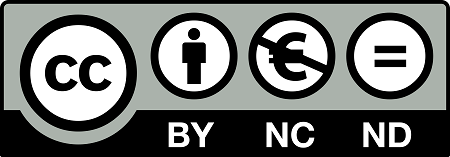
\includegraphics[width=4.2cm]{img/creativecommons.png}\\
		Esta obra se encuentra sujeta a la licencia Creative Commons\\ \textbf{Reconocimiento - No Comercial - Sin Obra Derivada}
	\end{sffamily}
\end{titlepage}

%----------
%	ÍNDICES
%----------	

%--
% Índice general
%-
\tableofcontents
\thispagestyle{fancy}

%--
% Índice de figuras. Si no se incluyen, comenta las líneas siguientes
%-
\listoffigures
\thispagestyle{fancy}

%----------
%	TRABAJO
%----------	

\pagenumbering{arabic} % numeración con múmeros arábigos para el resto de la publicación	


%----------
%	COMENZAR A ESCRIBIR AQUI
%----------	

\chapter{Información}
\section{Profesores}
\begin{quote}
Magistral: MARCELO GABRIEL BAGNULO BRAUN 

Prácticas: JUAN MAURICIO BARROSO FRESNEDA y MARCELO GABRIEL BAGNULO BRAUN:
\end{quote}

\section{Recursos}

\href{https://www.virtualbox.org/}{Oracle VM VirtualBox}

\href{https://www.nrl.navy.mil/itd/ncs/products/core}{Networks and
Communication Systems Branch}

\url{https://www.youtube.com/watch?v=eow0I39diug}

\url{https://www.youtube.com/watch?v=7wVJQTu5H3E}

\href{http://www.ingebook.com/ib/NPcd/IB_Escritorio_Visualizar?cod_primaria=1000193\&libro=6752}{Escritorio Virtualizar}

\href{https://padlet.com/fvalera/8njxmoxyj4qgck6d}{Computer Networks}


\part{Teoría}
\chapter{TEMA 1}

\section{1.1 y 1.3 Internet o Red de ordenadores}

  Conjunto de ordenadores interconectados de tal forma que pueden
  intercambiar información. Para los creadores de aplicaciones
  distribuidas es el servicio de comunicación que nos permite enviar y
  recibir mensajes mediante una API.

  Hoy en día casi cualquier cosa se puede conectar a internet, por
  tanto, el término de red de computadoras queda desactualizado, por
  tanto, en la jerga de internet todos los dispositivos que se conectan
  se denominan host o sistemas terminales.

  \begin{itemize}
  \item
    Actualmente ya no son solo ordenadores, hay mucha variedad de
    dispositivos.
  \item
    Infraestructura de comunicación:

    \begin{itemize}
    \item
      Dispositivos, que corren apps que conectan con la red. Hosts = end
      systems.
    \item
      Conmutadores = Packet switches y routers.
    \item
      Enlaces de comunicación, conectan los dispositivos con los router
      y los routers entre ellos, no es necesario conectar todos con
      todos.

      \begin{itemize}
      \item
        Los enlaces entre routers deben ser más rápidos que los enlaces
        entre router-dispositivo, ya que el router transmite muchos
        paquetes a la vez.
      \item
        La multiplexación estadística es la usada en la conmutación de
        paquetes, que asigna el uso del canal bajo demanda, es decir, no
        transmite de forma constante. Asigna dinámicamente los
        intervalos de tiempo de transmisión entre los terminales activos
        para no desaprovechar la capacidad del canal.
      \item
        FDM: multiplexación en frecuencias, es el usado en radio en la
        conmutación de circuitos
      \item
        La multiplexación por división de tiempo -- TDM tiene un tiempo
        de enlace asignado, por lo que se tarda igual independientemente
        de que haya más personas queriendo enviar información.
        Desaprovecha la capacidad del enlace, ya que dedica todo el
        ancho de banda del canal al transmisor en cada ranura de tiempo.
      \end{itemize}
    \item
      Network = Red, conjunto de dispositivos, routers y enlaces de una
      organización.
    \end{itemize}
	\pagebreak
  \item
    El host rompe los mensajes en paquetes de datos de aprox. 1500 bytes
    para ser transmitidos con un encabezado que permite indicar el
    destinatario y a la red llevarlos. Una vez dividido se transmite por
    un enlace al router, así con la cabecera sabe dónde reenviar otro
    router, ahí hasta llegar al destino.

    \begin{itemize}
    \item
      Store and forward: Debe llegar el paquete completo al router antes
      de transmitirlo por el siguiente enlace.
    \end{itemize}
  \item
    Funciones clave de los nodos de la red:

    \begin{itemize}
    \item
      Forwarding -- Reenvío: Es una acción local, que se encarga de
      mover los paquetes que llegan por el enlace de entrada al enlace
      de salida correspondiente.
    \end{itemize}
  \item
    Routing -- Enrutamiento: Es una acción global, consiste en
    determinar la ruta desde el origen hasta destino que seguirán los
    paquetes mediante algoritmo de enrutado.
  \end{itemize}
  \begin{figure}[H]
	\ffigbox[\FBwidth]
	{\caption{Circuit switching}}
	{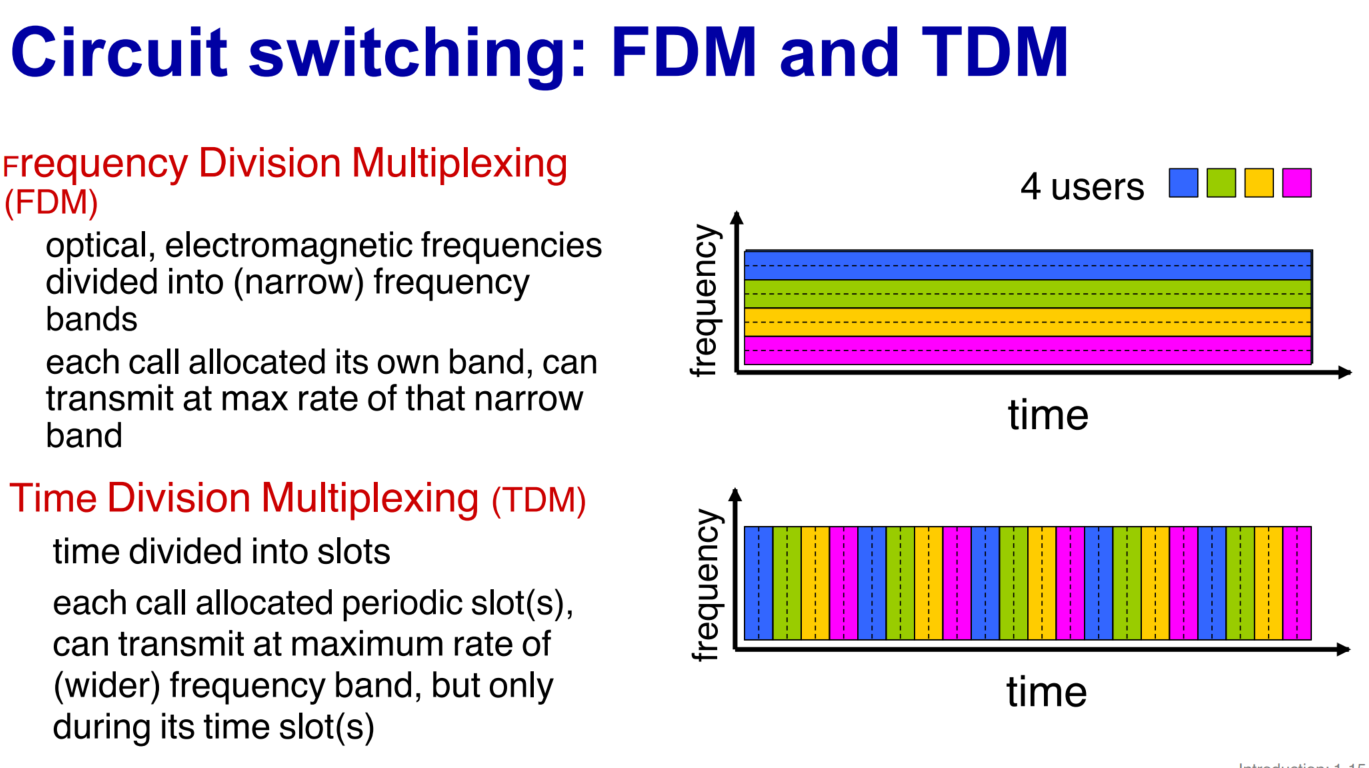
\includegraphics[scale=.25]{Untitled.png}}
\end{figure}

\section{1.2 Las fronteras de la red}

  Redes de acceso

  Medios físicos

  \pagebreak
\subsection{Arquitectura de la red}

	Hoy en día usamos principalmente dos redes de comunicación, la red
	telefónica e internet.

	\begin{itemize}
	\item
	Conmutación de circuitos: Conceptualmente hablando en la red
	telefónica se crea un cable que te conecta la llamada y cuando
	finaliza se despliega para dejar disponible los recursos para formar
	otra conexión. Se usa multiplexación de división en el tiempo y
	frecuencia. Usa toda la capacidad del enlace para el intercambio.
	\item
	Conmutación de paquetes: Los datos se trocean y se les agrega un
	encabezado con la dirección de destino y se envía, los routers y
	conmutadores miran la dirección y lo envía por su camino hasta llegar
	al destino. Utiliza multiplexación estadística. Se comparten todos los
	recursos en tiempo real.
	\end{itemize}

\section{1.5 Protocolos}

	Definen el formato, orden de enviado y recepción de mensajes entre las
	entidades de la red y acciones tomadas en la transmisión de mensajes.
	Hay tantos dispositivos y apps interconectados, cada uno distinto, para
	que pueda funcionar todos deben hablar un lenguaje común, los protocolos
	permiten acordarlo. Están en todas las conexiones, control de envíos y
	recepción de datos.

\subsection{Modelo de capas:}

	\begin{itemize}
	\item
	Cada capa siente que la comunicación es horizontal, sin embargo, la
	implementación es vertical. Cada capa implementa un servicio y el
	inverso
	\item
	El origen y destino implementan todas las capas. En el origen va de
	arriba hacia abajo, en los intermedios sube y baja, y en el destino
	sube las capas.
	\item
	Los enrutadores - routers implementan la capa red, enlace y física.
	\item
	Los conmutadores - switch implementan enlace y física.
	\pagebreak
	\item
	Capas:

	\begin{itemize}
	\item
		Aplicación: Los propios programas que quieren enviar y recibir
		datos. Soporta aplicaciones distribuidas. Pone el mensaje.
	\item
		Transporte: Multiplexación y desmultiplexación de datos para poder
		utilizar distintas aplicaciones. Transferencia de datos entre
		procesos. Pone un encabezado para identificar la aplicación, pasa a
		llamarse segmento.
	\item
		Red: Enrutamiento de datagramas de origen a destino: IP, protocolos
		de enrutamiento. Concatena saltos para llevar los paquetes desde el
		origen hasta el destino. Pone otro encabezamiento que indica la
		localización del origen y destino, pasa a llamarse datagrama.
	\item
		Enlace: Corrige y detecta errores de la transmisión, transfiere los
		datos a la entidad de la red vecina, en conexiones a 1 salto. Pone
		otro encabezamiento que indican el siguiente salto en la red, pasa a
		llamarse trama.
	\item
		Física: Traduce bits a ondas que se envían por el cable y viceversa.
	\end{itemize}
	
	\end{itemize}


\section{1.4 Retraso}

El tiempo que pasa desde que el paquete es recibido por el router hasta
que llega al destino.
$$d_{nodal}= d_{procesado}+d_{cola}+d_{transmisión}+d_{propagación}$$


  Tipos:

  \begin{itemize}
  \item
    Procesamiento, comprobar error de bit y determinar el enlace de
    salida.
  \item
    Cola, espera a ser transmitido por un enlace de salida.

    \begin{itemize}
    \item
      Intensidad de tráfico = \(\frac{L\cdot a}{R}\)

      \begin{itemize}
      \item
        L: tamaño paquete
      \item
        a: ratio de llegada del paquete
      \item
        R: ancho de banda
      \end{itemize}
    \end{itemize}
  \item
    Trasmisión: En transmitir los datos, volcarlo en el enlace.
    \(\frac{L}{R}\)

    \begin{itemize}
    \item
      L: bits del paquete o mensaje.
    \item
      R: ancho de banda del enlace. Bits/seg
    \end{itemize}
  \item
    Propagación: Tiempo que tarda en transmitirse por el enlace.
    \(\frac{d}{s}\)

    \begin{itemize}
    \item
      d: distancia del enlace. metros
	\item
	  s: velocidad de propagación. Metros/seg
    \end{itemize}
  
  \end{itemize}

\section{1.4 Traceroute:}

  Método para conocer el retraso o perdida de datos.

  Consiste en enviar 3 paquetes a destino, con tiempos de vida, de menos
  a más. Cuando su tiempo termina vuelve y sabe cuánto tarda en cada
  salto, al aumentar va llegando más lejos. Cuando hay un gran salto de
  ms (milisegundos) podemos analizar la fuente.

\section{1.4 Perdida}

Cuando la capacidad del buffer se termina o se han enviado mal, y
dependiendo del protocolo:

\begin{itemize}
\item
  Se pierde, se descarta lo que no entra.
\item
  Pide al emisor que lo reenvíe.
\end{itemize}

\section{1.4 Throughput}


  Tasa de procesamiento, la capacidad de un sistema para volcar datos
  para transmitir. \(\frac{Bits}{tiempo}\).

  \begin{itemize}
  \item
    Se caracteriza por el peor caso:

    \begin{itemize}
    \item
      Instantáneo: En un momento determinado
    \item
      Medio: De media.
    \end{itemize}
  \end{itemize}

  Cuello de botella / bottleneck: Cuando un enlace de una ruta restringe
  el Throughput de la ruta, dado que en esa ruta habrá un enlace de
  menor capacidad o que esté saturado.

  Se toma para los cálculos el mínimo entre el \(\frac{R}{10}\),
  \(R_{emisor}\) o \(R_{receptor}\).
  \begin{figure}[H]
	\ffigbox[\FBwidth]
	{\caption{Throughput}}
	{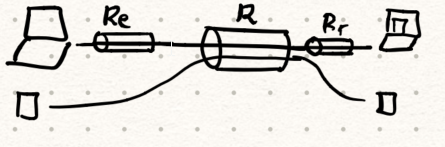
\includegraphics[scale=.5]{Untitled 2.png}}
\end{figure}

    Como R recibe muchas conexiones puede haber cuello de botella en
    \(R_e\) y \(R_r\).

\chapter{TEMA 2: Application Layer}

\section{2.1 Principios de las aplicaciones de red}

    Crear una aplicación de red:

    \begin{itemize}
    \item
      Son aplicaciones distribuidas, que necesitan intercambiar
      información para funcionar.
    \item
      Hay que crear la aplicación del cliente para los distintos
      dispositivos y servidor, y ejecutarla.
    \item
      No es necesario modificar los elementos de la red, los usuarios
      son los que hacen que funcione la red utilizando la aplicación.
    \end{itemize}

	Cliente: El que envía datos o inicia la comunicación.

	Servidor: El que recibe o espera la comunicación.

	Proceso: programa que se ejecuta.

    \begin{itemize}
    \item
      dentro de un host.
    \item
      dentro del mismo host, dos procesos se comunican mediante la
      comunicación entre procesos.
    \item
      procesos en diferentes hosts que se comunican mediante intercambio
      de mensajes.
    \end{itemize}

	
\subsection{Formas de estructurar las aplicaciones:}

    Paradigma cliente-servidor:

    \begin{itemize}
    \item
      Servidor: Su función es brindar servicio. Deben estar siempre
      disponible y accesible. Dirección IP permanente.
    \item
      Cliente: Solo se conecta cuando necesita algo.
    \end{itemize}

	Arquitectura peer-peer (igual-igual): Las comunicaciones se hacen
    directamente entre usuarios, sin pasar por un servidor.

    \begin{itemize}
    \item
      Cliente: No siempre en línea, pides servicio a otro usuario y
      provees servicio a otros usuarios.
    \item
      Auto escalabilidad: Cuando más clientes más capacidad de servicio.
    \end{itemize}

\subsection{Sockets:}


    Interfaz entre la capa de aplicación y transporte, dentro de esta
    última.

	Se utiliza para comunicar una aplicación con otra, en cada
    dispositivo hay un shocket para esa aplicación.

	Permite al sistema identificar cada aplicación, cuando se reciben
    datos se pasan al correcto.

	Un puerto no identifica de forma única la aplicación, hasta que se
    le asigna uno.

	Puerto: Identifica al socket del dispositivo con 16 bits. Hay un
    rango asignado a aplicaciones bien conocidas.

\subsection{Protocolo de la capa de aplicación:}

    Define:

    \begin{itemize}
    \item
      Tipos de mensajes intercambiados.
    \item
      Sintaxis del mensaje.
    \item
      Semántica del mensaje.
    \item
      Reglas de cuándo y cómo los procesos envían y responden los
      mensajes.
    \end{itemize}

	Tipos:

    \begin{itemize}
    \item
      Protocolos abiertos: Todo el mundo tiene acceso a la definición.
    \item
      Protocolos de propietario: Propios de la aplicación.
    \end{itemize}

	
\subsection{Necesidades del servicio de transporte:}

  Dependiendo de la aplicación puede ser más o menos susceptible.

  \begin{itemize}
  \item
    Integridad de datos: Los datos no hayan sido alterados, ya sea por
    fallos o interferencias. Aplicación de envío de datos son muy
    susceptibles y las de audio o video pueden tolerar perdidas.
  \item
    Temporalidad: El tiempo que tarda en llegar. Las de telefonía o
    videojuegos necesitan baja latencia.
  \item
    Ancho de banda: Cuantos datos puede recibir y enviar. Algunas
    necesitan mucha capacidad, otras se adaptan a lo que hay.
  \item
    Seguridad: Encriptado, integridad, \ldots{}
  \end{itemize}

\section{2.4 DNS -- Domain Name System}

    Directorio/Base de datos distribuida/espacio de nombres global, en
    formato amigable para el usuario, que nos permite mediante un
    protocolo obtener la IP.

	Cada nombre está asignado a una IP, es una manera más intuitiva
    dado que una dir IP son 32 bits, 4 números entre 0-255. No es
    asequible para el usuario, por eso se crea el DNS que permite
    asignar nombres a dispositivos amigables para el usuario.

	Es un protocolo de la capa de aplicación.

	Diagrama paquete
	\begin{figure}[H]
		\ffigbox[\FBwidth]
		{\caption{Diagrama paquete DNS}}
		{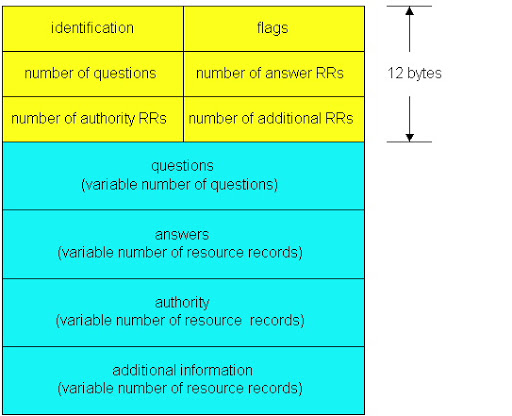
\includegraphics[scale=.4]{Untitled.jpeg}}
	\end{figure}
	Jerarquía:

    \begin{itemize}
    \item
      Servidor raíz: Capaces de resolver el mapeo de cualquier nombre
      del sistema de nombres de dominio.

      \begin{itemize}
      \item
        Conoce los servidores que contienen la información de los
        subdominios para todo el espacio de nombres.
      \item
        Hay 1 maestro, pero hay muchas copias distribuidas por el mundo.
      \end{itemize}
    \item
      TLD -- Top Level Domain - Dominios de alto nivel: Tienen autoridad
      sobre todo un subdominio (.com/.edu/.es/\ldots).
    \item
      Autoritario: Donde se almacena la información de mapeo de nombre y
      su IP. Conoce la IP para una determinada terminación de nombres
      (uc3m.es) propios de la organización.
    \item
      Local: Fuera de la jerarquía, es el nivel más bajo. Responsable de
      subdominios de bajo nivel. Se consulta para resolver los nombres y
      lo poseen las empresas para su propia administración.
    \end{itemize}

	Resolución de nombre DNS:

    \begin{itemize}
    \item
      Consulta iterativa:

      \begin{itemize}
      \item
        Se busca una DNS a la que queremos acceder.
      \item
        Como no se conoce la IP, se llama al DNS resolver para
        obtenerla.
      \item
        Llama al server local, si la conoce nos la envía, pero si no
        consulta al servidor raíz.
      \item
        El servidor raíz nos indica el servidor que conoce ese
        subdominio.
      \item
        Accedemos a ese servidor que nos manda a otro que sepa más
        profundo el subdominio o nos envía la IP.
      \end{itemize}
    \item
      Consulta recursiva:

      \begin{itemize}
      \item
        Consiste en hacer una sola consulta y que la siguiente consulta
        la haga el servidor consultado al siguiente en la jerarquía
        hasta llegar al local.
      \end{itemize}
    \end{itemize}

	Para introducir un nombre nuevo se llama al registrador DNS, que
    introduce 2 registros en un Servidor autoritario, uno de tipo A y
    otro de tipo NS.

	Seguridad:

    \begin{itemize}
    \item
      Ataques DDoS: bombardear al servidor raíz con tráfico.
    \item
      Ataques de redirección:

      \begin{itemize}
      \item
        Hombre en el medio: Interceptar las consultas.
      \item
        Envenenamiento de DNS: send bogus relies to DNS server, which
        caches.
      \end{itemize}
    \end{itemize}

\section{2.7 Programación de sockets: creación de aplicaciones de red}

  \begin{itemize}
  \item
    En UDP
  \item
    En TCP
  \end{itemize}

\chapter{TEMA 3: Transport Layer}

\section{3.1 Capa de transporte y sus servicios}
Entre la capa de red y aplicación.

Mejora la capa de red, ofrece un canal lógico de comunicación entre
    aplicaciones de distintos dispositivos.

	Solo está presente en los extremos, emisor y receptor.

\subsection{Acciones de los protocolos de transporte:}


    Emisor: Recibe los bits del mensaje de la aplicación los segmenta y
    les añade una cabecera que indica el origen y destino.

	Receptor: Recibe los segmentos y los une todos para formar el
    mensaje completo y lo pasa a la aplicación.

	
\subsection{Servicio:}


    Orientado a conexiones: Se envía un mensaje de señalización y el
    receptor acepta o rechaza. Si acepta se abre un canal de conexión.

	No orientado a conexiones: Se abre el canal y ya. Llegan los
    mensajes.

	
\section{Principales protocolos de transporte:}
\subsection{3.5 TCP - Transmission Control Protocol:}


    Orientado a conexiones: Hace que el cliente y el servidor
    intercambien la información de control de capa de transporte entre
    si antes de que empiecen a fluir los mensajes del nivel de
    aplicación. Este procedimiento denominado de negociación, de
    reconocimiento o de establecimiento de la conexión alerta al cliente
    y al servidor, permitiéndoles prepararse para el intercambio de
    paquetes, se conectan los sockets del emisor y del receptor, de esta
    manera lo que entra por un lado sale por el otro.

    \begin{itemize}
    \item
      Solo soporta comunicaciones 1 a 1, un emisor y un receptor. Crea
      un canal bidireccional entre ambos en la misma conexión.
    \end{itemize}
  \pagebreak
    Ofrece servicio confiable, los segmentos llegan íntegros y en orden.
    Se envía redundancia cíclica del mensaje en la cabecera para ver al
    llegar si ha fallado o ha habido interferencias, pero no ataques
    (habrían pensado en cambiarlo).

    \begin{itemize}
    \item
      Lo malo es que parte del ancho de banda usar para redundancia,
      si falla se reenvía y el resto de segmentos debe esperar a que
      llegue.
    \end{itemize}

	Control de flujo, el emisor no satura al receptor, y congestión.

	No proporciona: temporización, ancho de banda garantizado,
    seguridad.

	Servicio fiable de transferencia de flujos de bytes, a diferencia de
    UDP que es de paquetes.

	Recibe datos de la capa de aplicación y puede:

    \begin{itemize}
    \item
      Segmentar y enviar.
    \item
      Esperar para hacer un paquete más grande y envía, pero crea
      retardo si espera.
    \end{itemize}

	Si el paquete es demasiado pequeño, la cabecera ocupa más que los
    propios datos.

    \begin{itemize}
    \item
      Los paquetes son costosos en overhead, pero para algunas
      aplicaciones son necesarios, ya que no pueden esperar hasta que
      lleguen a crear un paquete más grande.
    \end{itemize}

	Cuanta más carga en la red es más importante la eficiencia, cuesta
    más introducir paquetes al haber retraso de cola.

	TCP siempre envía MSS:

    \begin{itemize}
    \item
      MSS: Máximo tamaño de segmentación.
    \item
      El receptor tiene pipeline que permite una ventana deslizante de
      tantos paquetes como quepan en el buffer, por si se corrompe
      alguno.
    \item
      Usa un método parecido al Go-back N, recibe asentimiento del
      último número de secuencia que se recibió en orden en el receptor
      y si se pasa el temporizador envía solo el más viejo. El receptor
      almacena en el buffer los paquetes que recibe fuera de orden, pero
      sigue mandando la confirmación del que le falta en medio, y cuando
      lo recibe los pasa en orden a la aplicación.

	  \begin{figure}[H]
		\ffigbox[\FBwidth]
		{\caption{Envio mensajes en TCP}}
		{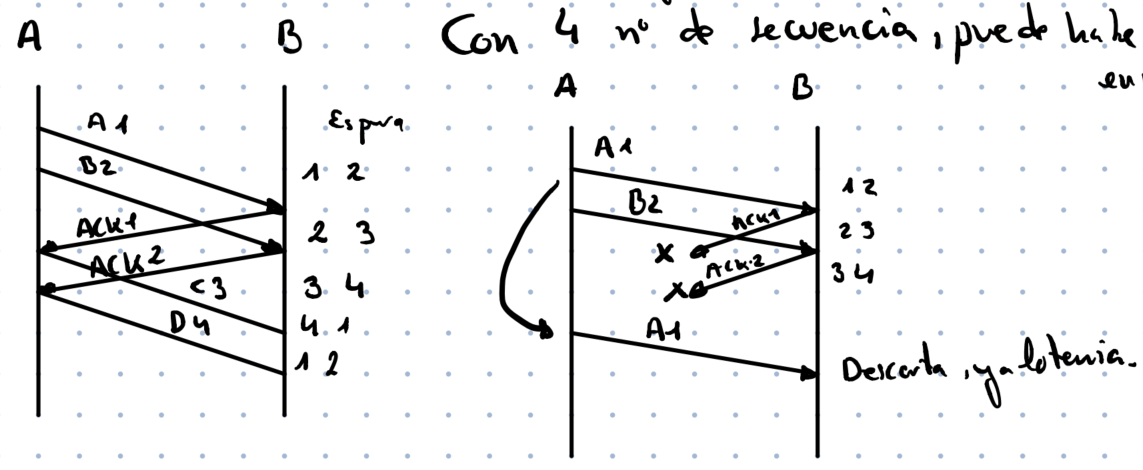
\includegraphics[scale=.25]{Untitled 3.png}}
	\end{figure}
    \item
      La unidad fundamental de transmisión es el byte, por ello a cada
      byte que transmita le asocia un numero de secuencia. Cuando se
      recibe un asentimiento, se ha tenido en cuenta la suma de los
      bytes de los datos.

      \begin{itemize}
      \item
        Si envió el paquete n.º 92 de 8 bytes, el asentimiento que reciba
        será el n.º 100, confirmando que ha recibido esos 8 bytes.
      \end{itemize}
    \end{itemize}

	Para tener n paquetes en vuelo necesitamos 2n números de secuencia.

	Segmentado: el control de flujo y congestión de TCP fijan el tamaño
    de la ventana. Hay buffers de emisión y recepción.

	Crea un segmento con:

    \begin{itemize}
    \item
      Puerto del origen y destino, los puertos identifican la
      aplicación.
    \item
      n.º secuencia: identifica el orden y evita duplicados. El número va
      aumentando según los bytes enviados, van asociados.
    \item
      n.º ack: Es el número de secuencia que espera recibir el receptor,
      para cuando intercambiamos datos.
    \end{itemize}
	\begin{figure}[H]
		\ffigbox[\FBwidth]
		{\caption{Segmento TCP}}
		{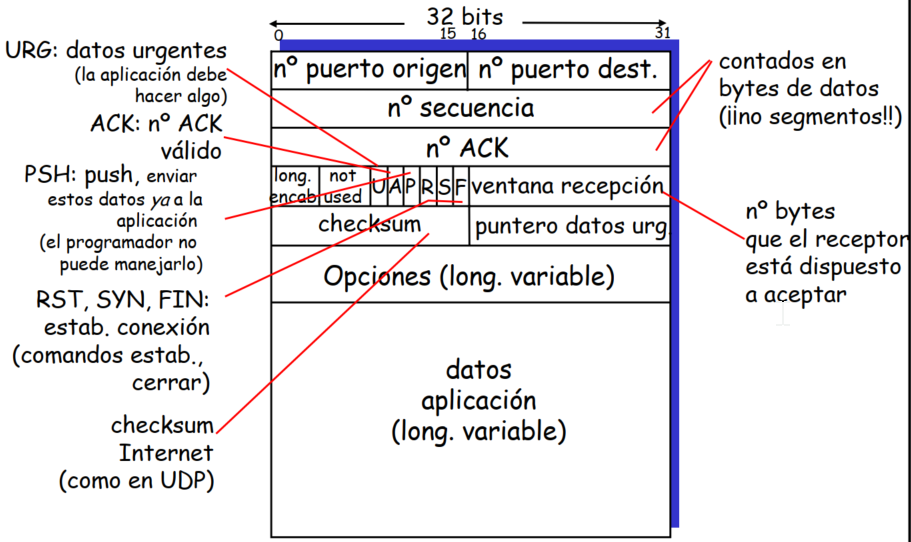
\includegraphics[scale=.4]{Untitled 4.png}}
	\end{figure}
	\pagebreak
	En la cabecera se pone el número de secuencia del propio paquete y
    además el número de secuencia que yo espero recibir si se quiere
    comunicar conmigo de vuelta.

    \begin{itemize}
    \item
      Cuando se envían datos bidireccionalmente, cada lado tiene su
      propio número de secuencia de tal manera que cada uno controla la
      llegada de sus propios datos y el otro confirma esos paquetes
      recibidos.
	  \begin{figure}[H]
		\ffigbox[\FBwidth]
		{\caption{Secuencia ACKs}}
		{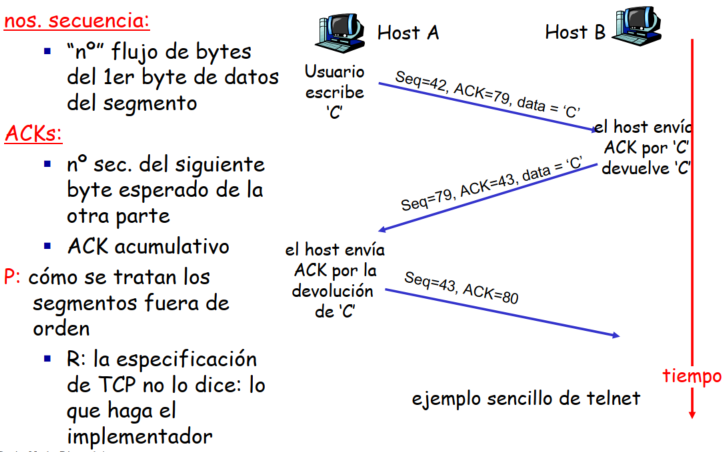
\includegraphics[scale=.45]{Untitled 5.png}}
	\end{figure}
    \end{itemize}

	Calcular el tiempo para el temporizador (timeout):

    \begin{itemize}
    \item
      Debe ser más que round trip time, ida y vuelta, pero este varía.
    \item
      Demasiado corto: Antes de recibir la confirmación ya he reenviado
      el paquete.
    \item
      Demasiado grande: Cuando no llega la confirmación espero demasiado
      tiempo. Aunque es mejor pasarse que quedarse corto
	  \begin{figure}[H]
		\ffigbox[\FBwidth]
		{\caption{Calcular EstimatedRTT}}
		{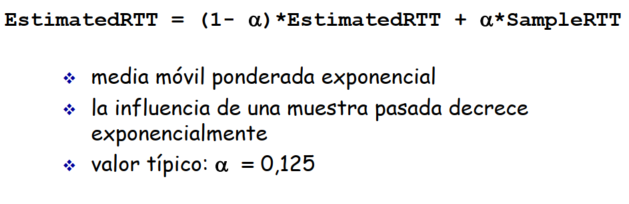
\includegraphics[scale=.45]{Untitled 6.png}}
	\end{figure}
	\begin{figure}[H]
		\ffigbox[\FBwidth]
		{\caption{Calculo de Timeout}}
		{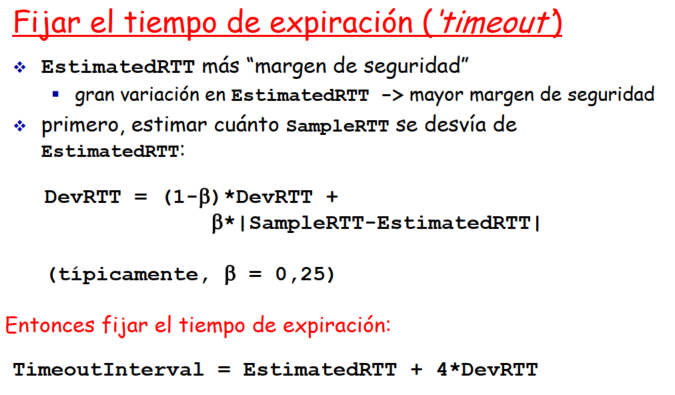
\includegraphics[scale=.45]{Untitled 7.png}}
	\end{figure}
    \item
      Cada vez que recibo un paquete, voy calculando la media ponderada
      móvil exponencial (las más recientes influyen más) de los RTT más
      un margen de seguridad según la variabilidad de los tiempos como
      tiempo límite para recibir un paquete.
    \end{itemize}

	Emisor:

    \begin{itemize}
    \item
      Crea un segmento con numero de secuencia según el byte del flujo
      de bytes.
    \item
      Se inicia un temporizador con tiempo de expedición:
      TimeOutArrival.

      \begin{itemize}
      \item
        Si pasa el tiempo, se reenvía y reinicia el temporizador.
      \item
        Si se recibe ACK de segmentos sin confirmación, desplazo la
        ventana, actualizo cuál es el más viejo e inicio temporizador si
        no hay ninguno para el más viejo.
      \end{itemize}
    \end{itemize}

	Receptor:

    \begin{itemize}
    \item
      Llegada de segmento en orden con el número de secuencia esperado,
      pero ya ha sido confirmado. Se espera hasta recibir el siguiente
      segmento, si no llega se envía ACK.

      \begin{itemize}
      \item
        El tiempo en enviar una confirmación: ¿Es de 500 ms?

        \begin{itemize}
        \item
          Cuando más grande es el tiempo que esperamos medido en número
          de confirmaciones de paquetes, el beneficio se va reduciendo
          en comparación a lo que aumenta el tiempo.
        \item
          Esto nos permite ahorrar confirmaciones, que congestionan la
          red.
        \item
          Lo mejor es enviar 1 confirmación de cada 2 paquetes.
        \end{itemize}
      \end{itemize}
    \item
      Llegada de segmento en orden con el número de secuencia esperado,
      pero hay otro segmento en orden esperando a ser confirmado. Se
      envía el ACK acumulativo de ambos, el más alto.
    \item
      Llegada de numero de secuencia fuera de orden mayor que el
      esperado. Se manda ACK duplicado inmediatamente del último en
      orden recibido, indicando el siguiente byte que esperamos.
    \item
      Llegada de segmento que completa parcialmente una laguna. Se envía
      ACK inmediatamente, suponiendo que el segmento empieza en el
      límite inferior de la laguna.
    \end{itemize}

	Retransmisión rápida: Se detectan segmentos perdidos por ACK
    repetidos. Si el emisor recibe 3 ACK por los mismos datos, supone
    que el segmento se ha perdido y reenvía ese segmento de inmediato,
    sin esperar a que termine el temporizador.

    \begin{itemize}
    \item
      Como el emisor envía varios segmento seguidos, si se pierde alguno
      llegaran varios ACK repetidos.
    \item
      El periodo de expiración a menudo es relativamente largo, lo que
      retrasa el reenvió de paquetes.
    \end{itemize}

	Cambia: Retardo -\textgreater{} Integridad.

\subsection{3.3 UDP -- User Datagram Protocol:}


    No orientado a conexiones: Como los sockets no están conectados, a
    la hora de enviar un mensaje hay que indicar quién es el destino, no
    crea un canal de comunicación.

	Mejor esfuerzo.

	Ofrece un servicio de comunicación no fiable, no hay garantías de
    que llegue bien o en orden.

	No proporciona: negociación, fiabilidad, control de flujo, control
    de congestión, temporización, ancho de banda garantizado, seguridad.

	La detección de errores es muy básica, avisa si hay fallos, pero no
    lo resuelve.

	Cabecera más ligera, a veces es mejor no hacer nada para no tener
    retardo, a pesar de no asegurar integridad.

	Al no haber establecimiento de la conexión, es más rápida.

	Al no tener control de congestión, puede disparar todo lo rápida que
    quiera.
\pagebreak
	Cabecera: Datagrama con

    \begin{itemize}
    \item
      Puerto de origen y destino.
    \item
      Length: Longitud en bytes del segmento UDP con el header.
    \item
      Checksum: Detectar errores, pero no los solventa.
	  \begin{figure}[H]
		\ffigbox[\FBwidth]
		{\caption{Diagrama paquete UCD}}
		{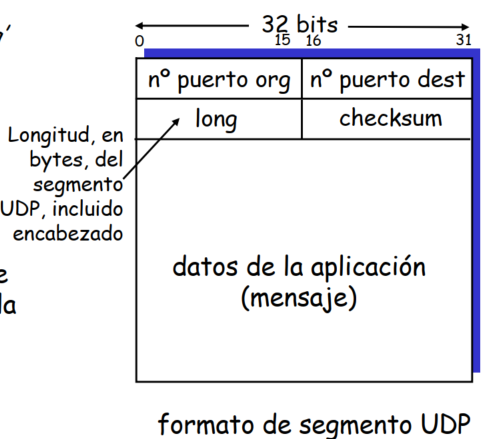
\includegraphics[scale=.45]{Untitled 8.png}}
	\end{figure}
    \end{itemize}

	Es utilizado para las DNS, para no sobrecargar los servidores raíz
    (no hay que enviar mensaje de solicitud para abrir conexión), como
    la integridad es importante la integridad a nivel de aplicación si
    falla o está corrupta se vuelve a hacer una consulta.

	Cambia: Integridad -\textgreater{} Retardo.

	UDP checksum: Numero añadido en el segmento de transporte para
    detectar errores. El emisor crea el checksum, el receptor lo
    recalcula y compara si son distintos, si lo son correcto y si no hay
    algún error.

    \begin{itemize}
    \item
      El emisor trata el contenido del segmento UDP (que incluye los
      campos de la cabecera UDP y las direcciones IP) como secuencias de
      16 bits enteros.
    \item
      Se van sumando los segmentos desde el primero de 16 en 16 bits, y
      si sale alguno de 17 bits cogemos el más significativo y se lo
      sumamos al mismo, 1º+2º, (1º+2º)+3º\ldots. Cuando hemos sumado
      todos hacemos complemento a uno, los 1 por 0 y 0 por 1.
    \end{itemize}
\pagebreak
\subsection{3.2 Multiplexación/ Demultiplexación:}


    El emisor multiplexa, añade la cabecera de transporte para ser
    demultiplexada después y vaya al socket correcto.
    El receptor demultiplexa, deshace la cabecera del segmento para
    entregarlo al socket correcto.

    \begin{itemize}
    \item
      Cada datagrama de la capa de red tiene la IP origen y destino con
      el correspondiente puerto de cada lado que identifica el socket.
    \end{itemize}

\subsection{3.4 Principios de transferencia de datos confiable:}

    Los servicios de transferencia confiable, consiguen que los datos
    lleguen y sin fallos.

	Para la capa de aplicación es como pasar los datos a un canal
    confiable, pero la capa de transporte realiza un protocolo para la
    transferencia de datos confiable y lo pasa a un canal no confiable o
    lo recibe de un canal no confiable(según el lado).

	Las características del canal no fiable determinarán la complejidad
    de transferencia de datos fiable.

	\begin{figure}[H]
		\ffigbox[\FBwidth]
		{\caption{Diagrama envio confiable}}
		{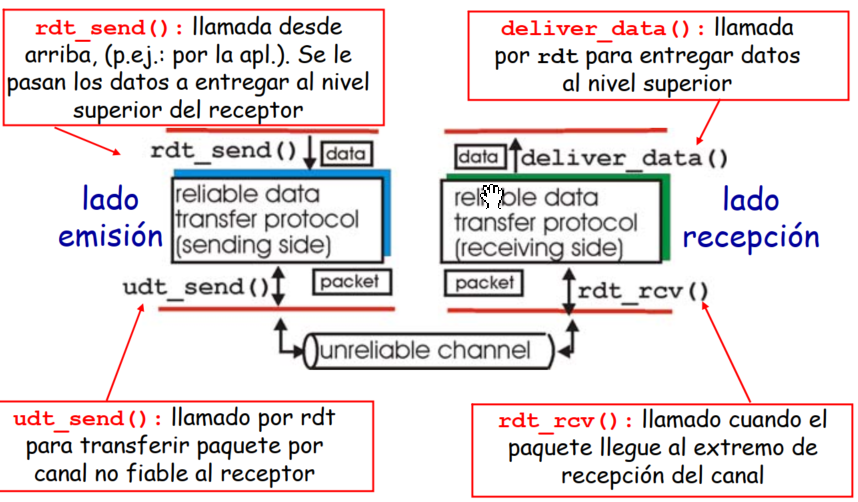
\includegraphics[scale=.35]{Untitled 9.png}}
	\end{figure}

	Terminología:

    \begin{itemize}
    \item
      rdt\_sent(): Pasa los datos la aplicación a la capa de transporte.
    \item
      udt\_send(): La capa de transporte transfiere el paquete por el
      canal no confiable al receptor (capa red).
    \item
      rdt\_rcv(): Cuando el paquete llega al extremo de recepción del
      canal (red -\textgreater{} transporte)
    \item
      deliver\_data(): La capa de transporte pasa los datos a la
      aplicación.
    \end{itemize}

	Se desarrollan los lados de emisor y receptor incrementalmente, se
    imponen una solución simple y vamos levantando la simplicidad con
    problemas del canal.

	Consideramos solo transferencia de datos unidireccional, pero
    funciona bidireccional de igual manera, es para simplificar.

	Se usan máquinas de estado finitas para representar emisor y
    receptor por separado: evento/acciones tomadas.

\subsubsection{rdt1.0: transferencia fiable en canal fiable.}

      Sin errores de bit, ni perdida de paquetes.

	  \begin{figure}[H]
		\ffigbox[\FBwidth]
		{\caption{rdt1.0}}
		{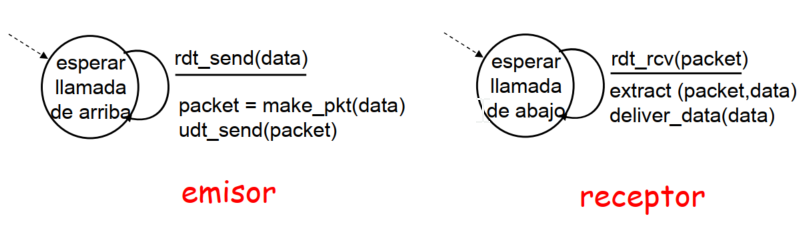
\includegraphics[scale=.45]{Untitled 10.png}}
	\end{figure}
   
      Emisor:

      \begin{itemize}
      \item
        Espera los datos de la aplicación, cuando los recibe crea un
        paquete y envía el paquete por el canal no confiable.
      \end{itemize}

	  Receptor:

      \begin{itemize}
      \item
        Espera recibir paquete, cuando lo recibe extrae los datos y los
        pasa la aplicación.
      \end{itemize}
\subsubsection{rdt2.0: canal con errores de bit.}

      El canal puede alterar bits del paquete, para eso se usa el
      checksum y se detectan.

	  Para resolver los errores, se usa:

      \begin{itemize}
      \item
        Asentimiento, confirmación o reconocimiento (Acknowledgements,
        ACK): El receptor indica que la recepción fue buena.
      \item
        Asentimiento negativo o reconocimiento negativo (NAK): El
        receptor indica que el paquete tenía errores. En este caso el
        emisor reenvía el paquete.
      \end{itemize}

	  Protocolo de parada y espera (stop and wait): Si se corrompe se
      envía una señal de respuesta negativa y el emisor envía de nuevo,
      si llega bien una respuesta positiva.
	  \begin{figure}[H]
		\ffigbox[\FBwidth]
		{\caption{rdt2.0}}
		{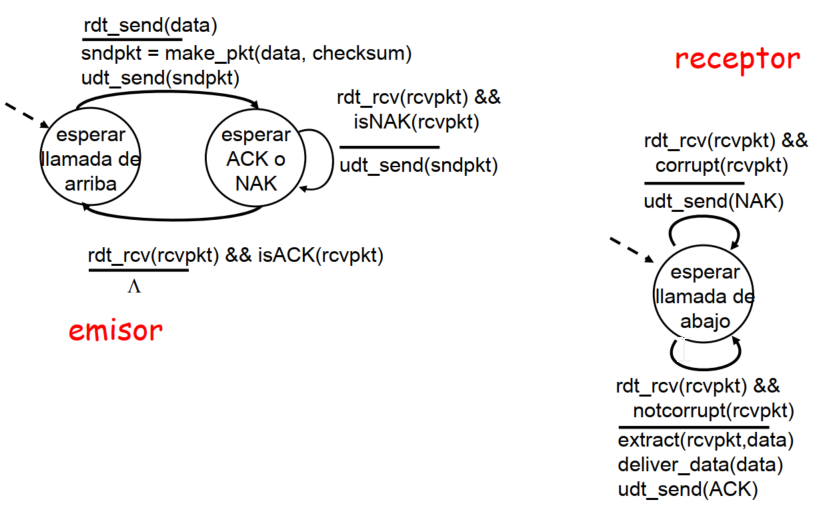
\includegraphics[scale=.45]{Untitled 11.png}}
	\end{figure}
	  Emisor:

      \begin{itemize}
      \item
        Espera recibir datos de la aplicación, cuando los recibe calcula
        el checksum y crea un paquete que incluye el checksum, entonces
        lo envía
      \item
        Espera un paquete del receptor ACK o NAK, si recibe ACK pasa a
        esperar datos de la aplicación, si recibe NAK envía de nuevo el
        paquete y espera otra vez ACK o NAK.
      \end{itemize}

	  Receptor:

      \begin{itemize}
      \item
        Espera un paquete del emisor, cuando lo recibe comprueba los
        datos con el checksum, si coincide envía ACK y pasa los datos a
        la aplicación, y si no coincide envía NAK.
      \end{itemize}

	  Pero qué pasa si se corrompe un asentimiento, no podemos asumir
      ACK (se pierden paquetes), ni NAK (se duplican paquetes). Para
      solucionarlo rdt2.1
\pagebreak
\subsubsection{rdt2.1: canal con errores de bit y manejo de ACK/NAK erróneos.}


      El emisor retransmite el paquete actual si ACK o NAK si no llegan
      bien.

	  El emisor añade un numero de secuencia a cada paquete, para
      detectar si se repite el paquete cuando se recibe.

	  Emisor:
	  \begin{figure}[H]
		\ffigbox[\FBwidth]
		{\caption{rdt2.1: Emisor}}
		{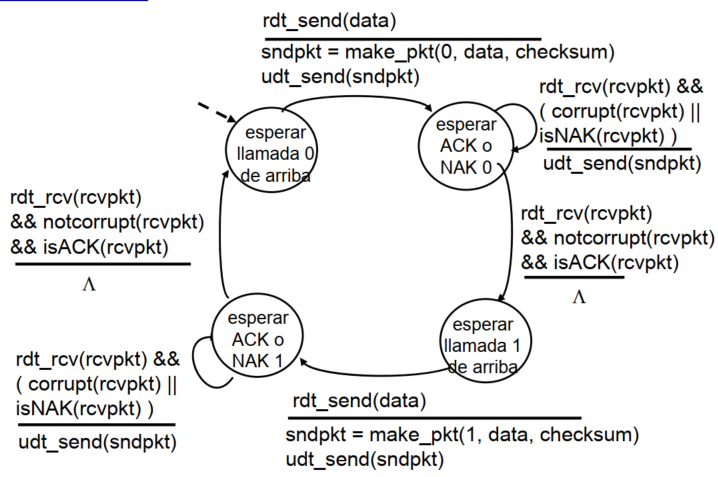
\includegraphics[scale=.45]{Untitled 12.png}}
	\end{figure}
      \begin{itemize}
      \item
        Espera datos de la aplicación para poner el número de secuencia
        0, cuando los recibe crea un paquete con el checksum, datos y el
        0.
      \item
        Espera recibir asentimiento con 0, si recibe ACK y no está
        corrupto pasa a espera datos para poner 1, si recibe NAK o está
        corrupto reenvía el paquete con 0.
      \item
        Espera datos de la aplicación para poner 1, cuando los recibe
        crea un paquete con el checksum, datos y el 1
      \item
        Espera recibir asentimiento con 1, si recibe ACK y no está
        corrupto pasa a espera datos para poner 0, si recibe NAK o está
        corrupto reenvía el paquete con 1.
      \end{itemize}

\pagebreak
      Receptor:
	  \begin{figure}[H]
		\ffigbox[\FBwidth]
		{\caption{rdt2.1: Receptor}}
		{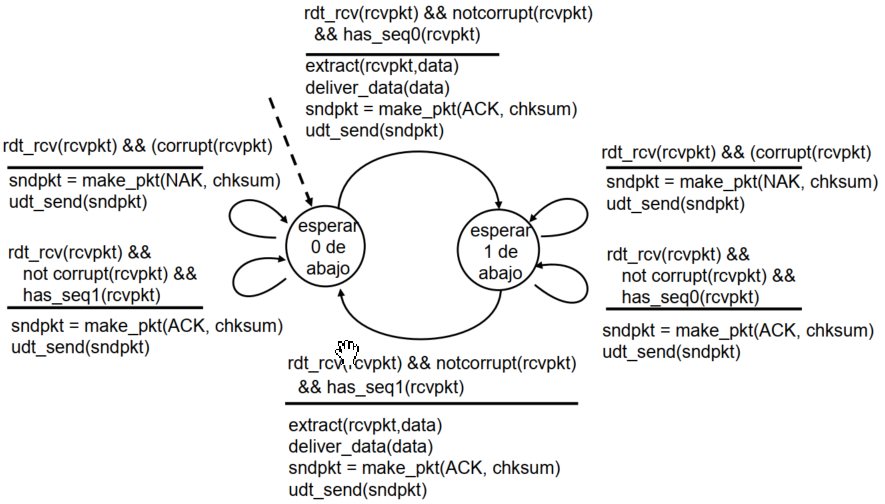
\includegraphics[scale=.45]{Untitled 13.png}}
	\end{figure}
      \begin{itemize}
      \item
        Espera paquete con numero de secuencia 0:

        \begin{itemize}
        \item
          Cuando recibe un paquete comprueba que el checksum no esté
          corrupto y numero de secuencia 0, si están bien ambos pasa los
          datos a la aplicación y crea un paquete con ACK y su checksum,
          por último, pasa a esperar un 1.
        \item
          Cuando recibe un paquete si no coincide el checksum con los
          datos, se envía NAK con su checksum, y sigue esperando un 0.
        \item
          Cuando recibe un paquete no corrupto (checksum correcto) y el
          número de secuencia es 1, se crea un paquete con ACK y su
          checksum (estaba duplicado)
        \end{itemize}
      \item
        Espera paquete con numero de secuencia 1:

        \begin{itemize}
        \item
          Cuando recibe un paquete comprueba que el checksum no esté
          corrupto y número de secuencia 1, si están bien ambos pasa los
          datos a la aplicación y crea un paquete con ACK y su checksum,
          por último, pasa a esperar un 0.
        \item
          Cuando recibe un paquete si no coincide el checksum con los
          datos, se envía NAK con su checksum, y sigue esperando un 1.
        \item
          Cuando recibe un paquete no corrupto (checksum correcto) y el
          número de secuencia es 0, se crea un paquete con ACK y su
          checksum (estaba duplicado)
        \end{itemize}
      \end{itemize}
\pagebreak
\subsubsection{rdt2.2: Un protocolo sin NAK.}


      La misma funcionalidad que rdt2.1, usando solo ACK

	  En lugar de NAK, el receptor envía ACK para el último paquete
      recibido bien indicando el número de secuencia del mismo.

	  Por lo tanto, el emisor si recibe un ACK de numero de secuencia
      incorrecta es NAK y retransmite.
	  \begin{figure}[H]
		\ffigbox[\FBwidth]
		{\caption{rdt2.2}}
		{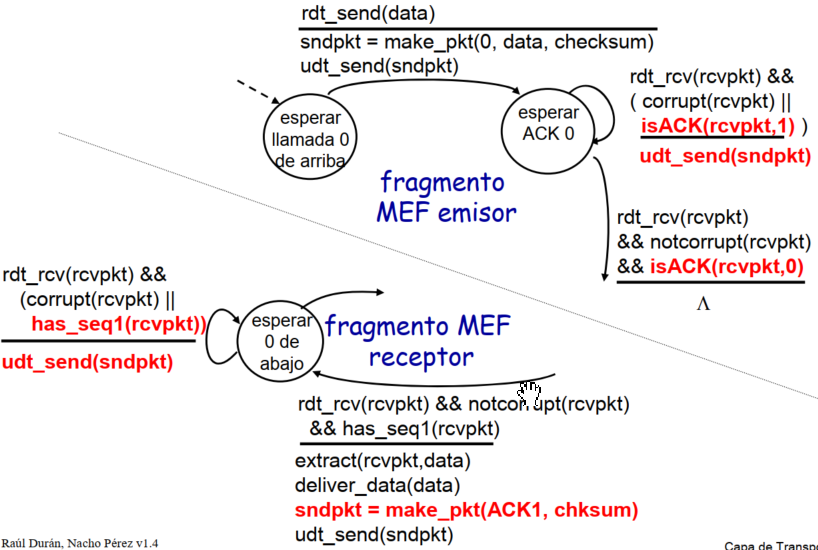
\includegraphics[scale=.45]{Untitled 14.png}}
	\end{figure}
\subsubsection{rdt3.0: Canales con errores y perdidas.}


      El emisor espera un tiempo razonable para recibir el asentimiento,
      si no se ha perdido.

	  El tiempo de espera es el round trip time, el tiempo que tarda un
      paquete en ir y volver.

	  Si se pasa el tiempo se reenvía, y si se reenvió antes de tiempo
      el número de secuencia lo identifica.

	  Usa números de serie, temporizador y checksum.

	  Emisor:

      \begin{itemize}
      \item
        Esperar datos para poner el 0, se reciben datos:

        \begin{itemize}
        \item
          Si se reciben datos de la aplicación se crea un paquete con el
          checksum y número de serie 0, se inicia un temporizador y se
          envía el paquete.
        \item
          Si se recibe un paquete del receptor no se hace nada.
        \end{itemize}
      \item
        Esperar asentimiento 0, se recibe un paquete del emisor:

        \begin{itemize}
        \item
          Si está corrupto el paquete o el número de serie recibido es
          1, no se hace nada.
        \item
          Si se pasa el temporizador se reenvía el paquete.
        \item
          Si no está corrupto y el número de serie es 0, se para el
          temporizador y pasamos a esperar datos de la aplicación para
          poner un 1.
        \end{itemize}
      \item
        Esperar datos para poner el 1, se reciben datos:

        \begin{itemize}
        \item
          Si se reciben datos de la aplicación se crea un paquete con el
          checksum y número de serie 1, se inicia un temporizador y se
          envía el paquete.
        \item
          Si se recibe un paquete del receptor no se hace nada.
        \end{itemize}
      \item
        Esperar asentimiento 1, se recibe un paquete del emisor:

        \begin{itemize}
        \item
          Si está corrupto el paquete o el número de serie recibido es
          0, no se hace nada.
        \item
          Si se pasa el temporizador se reenvía el paquete.
        \item
          Si no está corrupto y el número de serie es 1, se para el
          temporizador y pasamos a esperar datos de la aplicación para
          poner un 0.
        \end{itemize}
      \end{itemize}

	  \begin{figure}[H]
		\ffigbox[\FBwidth]
		{\caption{rdt3.0}}
		{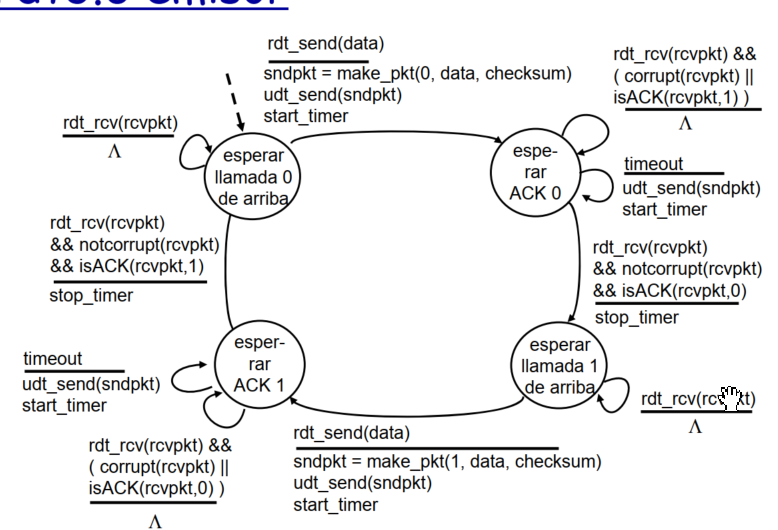
\includegraphics[scale=.45]{Untitled 15.png}}
	\end{figure}
	  \pagebreak
      Receptor: Es igual que en rdt2.2, se envía asentimiento positivo
      con checksum y numero de secuencia.

      \begin{itemize}
      \item
        Espero paquete con 0, recibo paquete del emisor:

        \begin{itemize}
        \item
          Está corrupto el paquete o número de serie 1, envía de nuevo
          la confirmación anterior para que mande de nuevo el paquete 0
          o el siguiente.
        \item
          Si no está corrupto y es un 0, pasamos los datos a la
          aplicación y enviamos al emisor el asentimiento con 0 y su
          checksum.
        \end{itemize}
      \end{itemize}

	  El problema de este mecanismo es el rendimiento, está la mayor
      parte del tiempo esperando respuesta.

	  
\subsubsection{Protocolos segmentados (pipelined protocols)}

    

      Se amplía el número de serie que se envía lo que nos permite
      aumentar el número de paquetes en vuelo.

	  Aunque necesitamos un buffer más grande en el emisor y/o el
      receptor.

	  Ventana: Numero de paquetes que puede haber en vuelo, sin
      confirmación.

	  Ventana deslizante: Se va olvidando de los confirmados y envía
      otro según confirma.

\paragraph{Go-Back-N}

    

        En el emisor hay un buffer y temporizador asociado a cada
        paquete.

        \begin{itemize}
        \item
          Si se pasa el tiempo reenvía todos los paquetes desde el más
          viejo.
        \item
          Según van llegando se desplaza la ventana y envía nuevos.
        \item
          Acepta duplicados, cuando recibe muchos iguales acabara el
          temporizador porque se ha perdido alguno.
        \end{itemize}

		En el receptor, solo sabe el paquete que está esperando, si
        llega lo pasa a la aplicación, pero si no es el esperado lo
        almacena en buffer o lo deja pasar.

        \begin{itemize}
        \item
          Se tiene un ACK acumulativo, le dice al emisor que ha recibido
          correctamente hasta cierto número de secuencia, el último en
          orden de secuencia. Mantiene el número 2 si no ha llegado,
          aunque reciba el 3 y 4.
        \end{itemize}

		Una ventaja es que, si se pierden confirmaciones, pero se recibe
        una con numero de secuencia superior antes de que pase el
        tiempo, el emisor entenderá que las perdidas han sido recibidas.

		\paragraph{Repetición selectiva (Selective repeat}

        Ventana de n paquetes, a cada uno con un temporizador y voy
        corriendo la ventana cuando se confirman y si no se confirman lo
        reenvía.

		El emisor solo reenvía paquetes para los que no reciba ACK,
        según se van recibiendo se va desplazando la ventana.

		El receptor envía ACK individual para cada paquete correcto, a
        diferencia de GBN no se queda solo con el número de secuencia
        del último correcto consecutivo. No mantiene numero 2 si recibe
        el 3 y 4, aunque no haya recibido el 2.

        \begin{itemize}
        \item
          En un buffer voy almacenando los paquetes que llegan en
          desorden y cuando tengo todos se pasan a la app.
        \end{itemize}

		Dilema: Como no necesariamente los acepta en orden, puede
        ocurrir que, al perderse todos los paquetes aceptados, aceptemos
        como nuevo los paquetes reenviados por el emisor al tener
        números de serie que correspondan a la ventana del receptor.


    Cada socket tiene asociado un buffer.

	El control de flujo y congestión reducen la velocidad de
    transmisión, para no saturar la red.

    $$TCP = \frac {nºpaquetes\cdot MSS}{RTT}$$

	Control de flujo: El emisor no saturará el buffer del receptor a
    base de enviar muchos paquetes seguidos. Se equilibra la velocidad
    de envío a la del receptor.

    \begin{itemize}
    \item
      El emisor debe controlar su velocidad de emisión para no saturar
      al receptor, para ello el receptor va enviando en sus
      confirmaciones cuanto buffer tiene libre, de esta manera se
      adapta.
    \item
      La velocidad de recepción de paquetes viene dada por el emisor, si
      el receptor capta los datos más lentos o tiene poco buffer, empieza
      a perder paquetes al no caber.
    \item
      Recibe más de lo que puede procesar.
    \end{itemize}
  
\pagebreak
\subsection{3.6 Principios del control de congestión}

    Congestión: hay más tráfico en una parte de la red de lo que es
    capaz de soportar.

    \begin{itemize}
    \item
      Normalmente son los enlaces los que se congestionan, cuando la
      multiplexación estadística se ve superada.
    \item
      A diferencia del control de flujo, la congestión es de la red, no
      del receptor.
    \end{itemize}

	Síntomas:

    \begin{itemize}
    \item
      Perdida de paquetes.
    \item
      Grandes retardos.
    \end{itemize}

	Tipos:

    \begin{itemize}
    \item
      Congestión crónica: Continúa en el tiempo, que dura. Se puede
      solucionar incrementando la capacidad, más enlaces.
    \item
      Congestión puntual: Momentánea. Se soluciona reduciendo la
      demanda, hacer que se envíe menos.
    \end{itemize}

	Formas de abordarla:

    \begin{itemize}
    \item
      Control de terminal a terminal: No hay retroalimentación de la
      red, se deduce por el retardo y las perdidas. Es el método de TCP.
    \item
      Control asistido por la red: Los routers proporcionan
      realimentación a los terminales. Indican a que tasa deben enviar
      los emisores.
    \end{itemize}

\subsection{3.7 Mecanismos de control de congestión de TCP}


    No se conoce como de congestionada esta la red, por lo que se va
    incrementando la tasa de transmisión poco a poco y cuando hay
    perdidas vuelvo a reducir.

    \begin{itemize}
    \item
      Es autocongestionante, lo sube hasta que se congestiona.
    \end{itemize}

	Incremento aditivo: Incrementamos el tamaño de ventana en 1 MSS cada
    RTT hasta que haya perdidas. +1 tamaño ventana

	Decremento multiplicativo: Dividimos el tamaño de ventana por 2
    cuando haya perdidas. Ventana/2

    \begin{itemize}
    \item
      En AIMD, corta por la mitad cuando recibe 3 ACK del mismo paquete
      y quita 1 cuando expira un temporizador.
    \end{itemize}

	AIDM: Algoritmo asíncrono distribuido para optimizar los ratios de
    congestión de la red y tienen propiedades de estabilidad.

	$$Tasa TCP \approx \frac {cwnd} {RTT} \frac {bytes}{sec}$$

	El emisor limita la transmisión: LastByteSent- LastByteAcked
    \textless{} cwnd

	ACK duplicados: Congestión moderada. Bajamos a la mitad +3 y
    subimos poco a poco. El umbral también se reduce a la mitad.

	Detectamos perdida por temporizador: Congestión severa. Bajamos el
    tamaño de ventana a 1 y volvemos a aumentar exponencialmente. El
    umbral se reduce a la mitad.

	Arranque lento: Comienza con tamaño de ventana pequeña, 1 MSS, pero
    no solo aumentan de 1 en 1, se va doblando por cada RTT hasta llegar
    a ssthresh (la mitad del valor de la ventana antes de la última
    perdida) y después continua linealmente hasta perdida.

	The Maximum Segment Size (MSS) is set to 1 in TCP Reno and Tahoe, in
    case of timeout detection, as the congestion is severe. However, in
    case of even less severe congestion detected by triple duplicate
    acknowledgement, the MSS size is reduced to 1 in TCP Tahoe and half
    in TCP Reno.
	\begin{figure}[H]
		\ffigbox[\FBwidth]
		{\caption{Control de congestión TCP}}
		{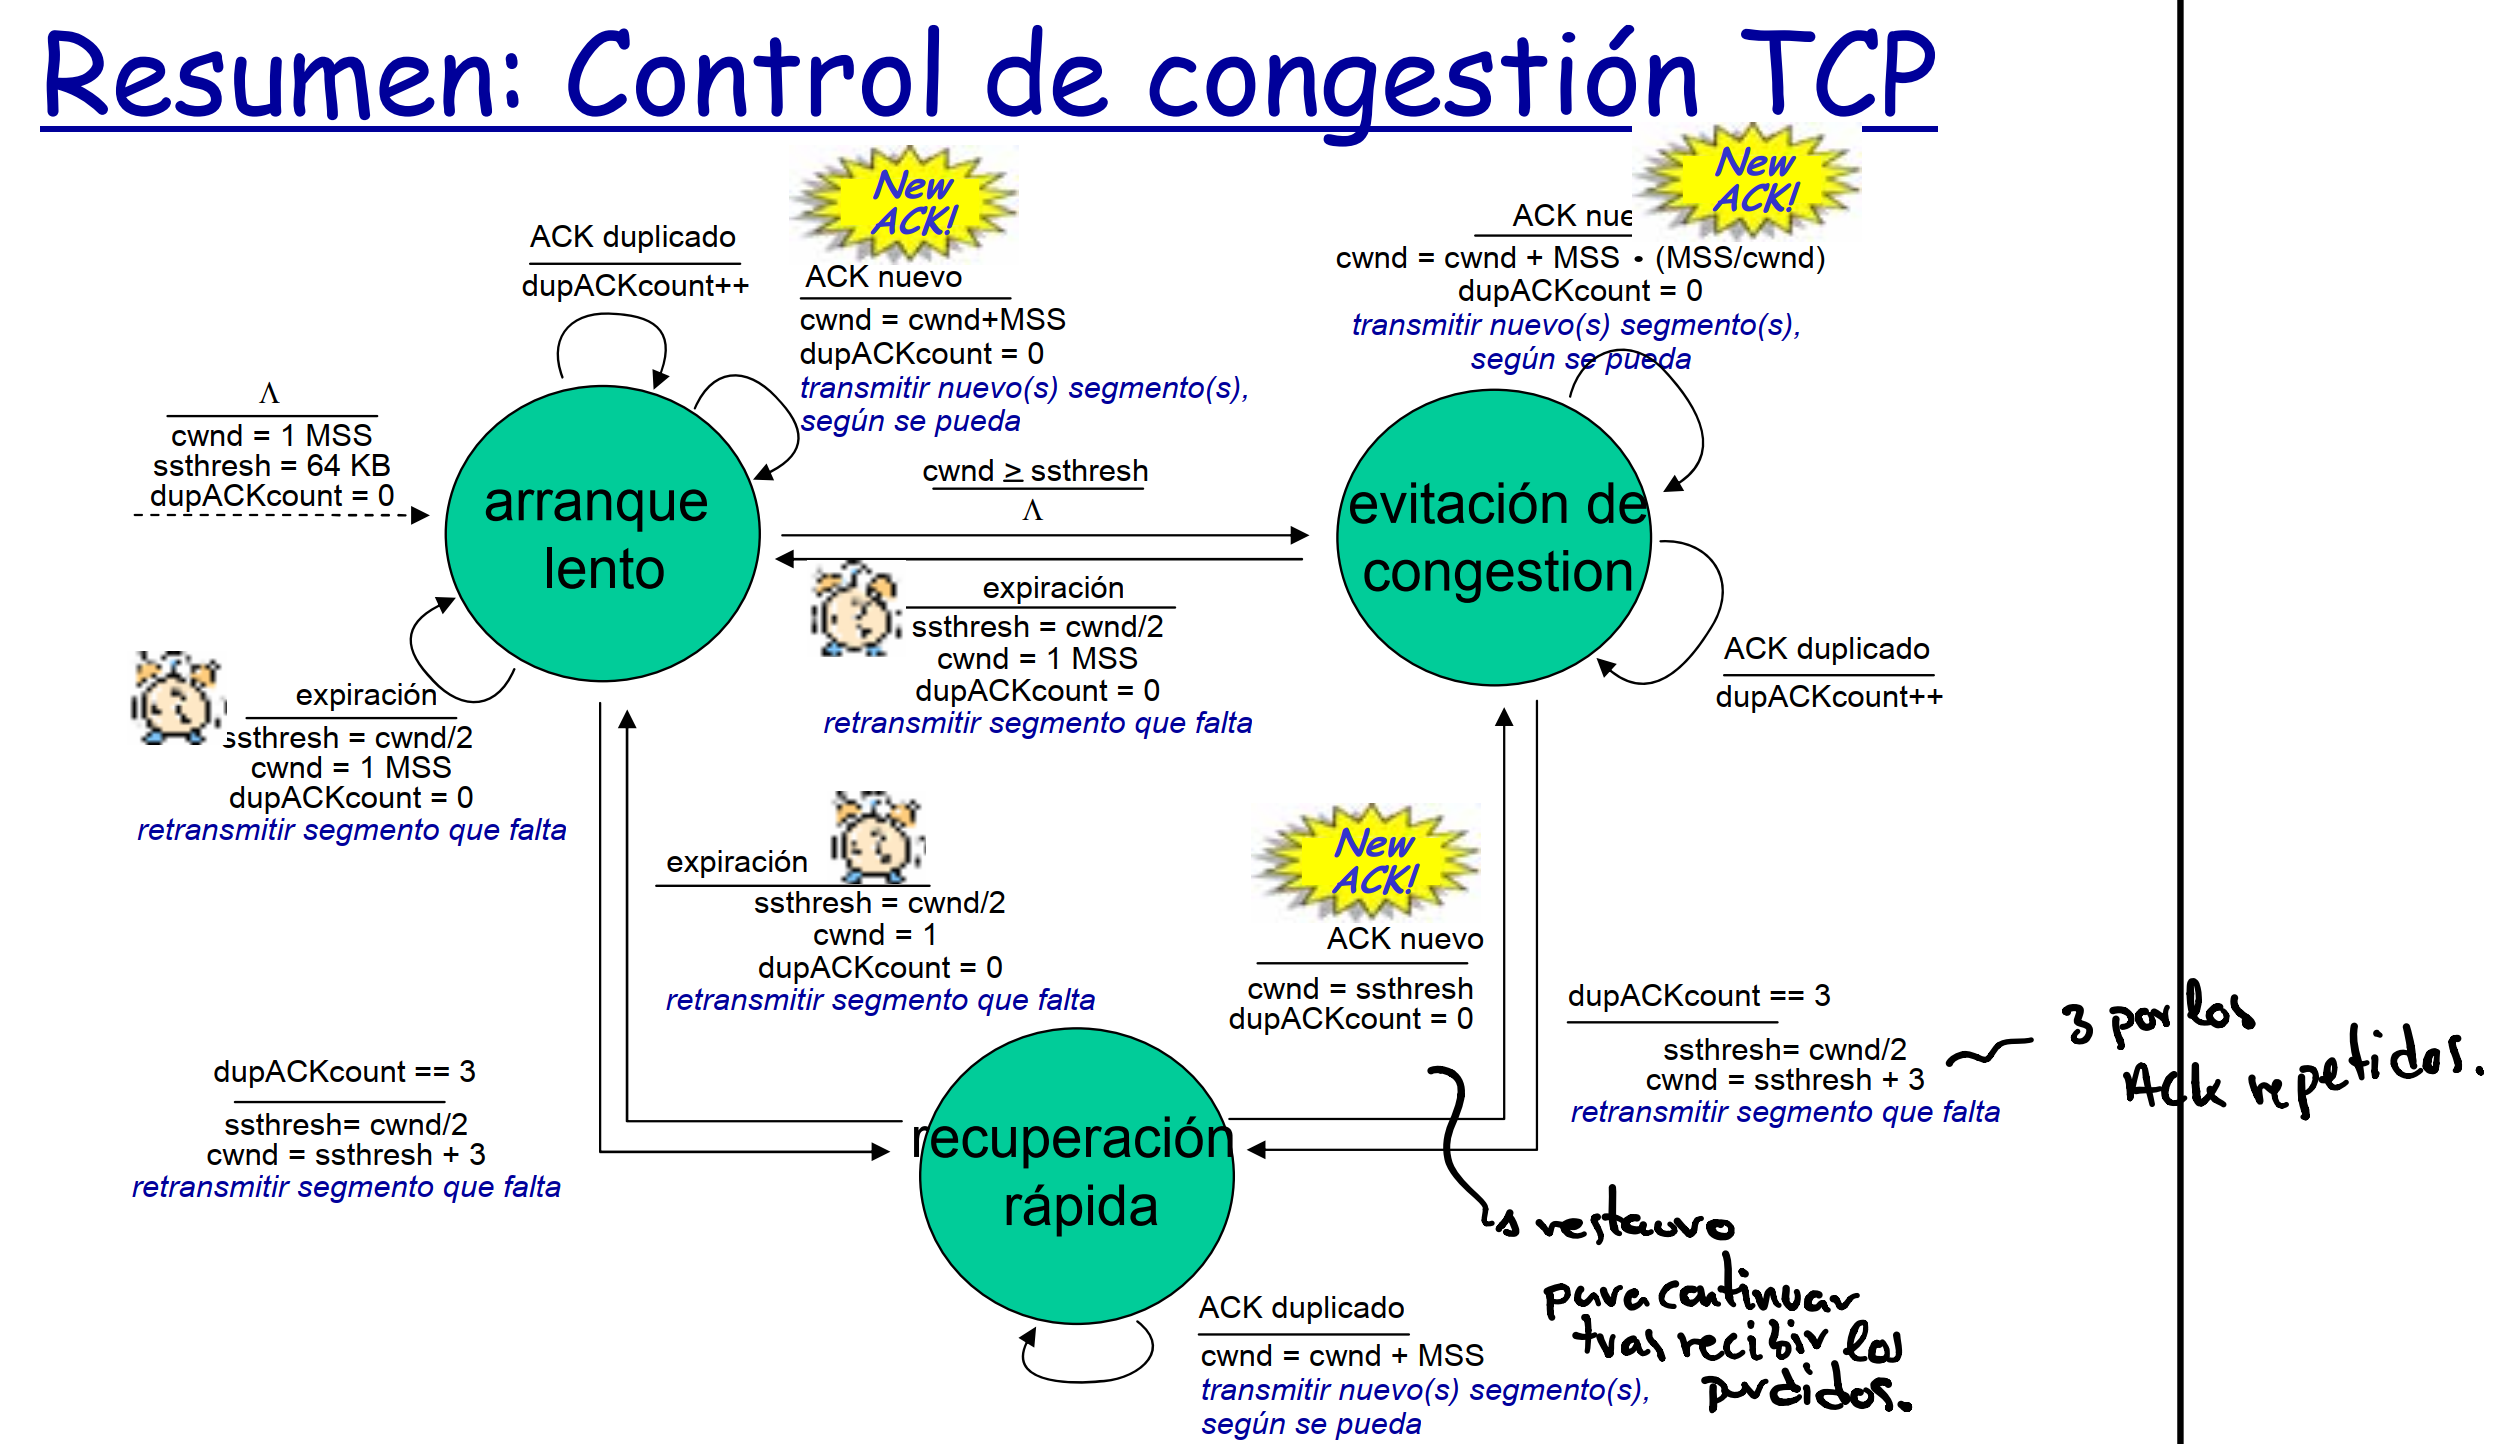
\includegraphics[scale=.15]{Untitled 19.png}}
	\end{figure}
    En arranque lento aumenta uno por cada segmento de la ventana, lo
    que al ocurrir para toda la ventana duplica.

    En evitación de congestión aumenta 1/ tamaño de la ventana, lo que
    hace que cuando se haya confirmado toda la ventana habrá aumentado
    uno completo.

\chapter{TEMA 4: Network Layer Data Plane}

\section{4.1 Overview of Network layer}

    Capa de red:

    \begin{itemize}
    \item
      Ofrece un canal lógico de comunicación entre hosts -- anfitriones
      conectados por un medio físico. Entrega los paquetes al destino
      indicado por su dirección IP, con los saltos que sean necesarios.
    \item
      Utiliza los servicios de la capa de enlace y los mejora para
      ofrecer mejor servicio a la capa de transporte.
    \item
      Transporta segmentos del host emisor al receptor.

      \begin{itemize}
      \item
        El emisor encapsula los segmentos en datagramas. Pone la
        dirección IP del dispositivo destino.
      \item
        El receptor entrega los segmentos a la capa de transporte.
      \end{itemize}
    \item
      Está presente en Routers y Hosts.
    \item
      El router examina los campos de la cabecera de todos los
      datagramas IP, para determinar a donde se debe enviar y cuál será
      el siguiente salto, pero la IP no cambia.
    \item
      Visión como dos planos:

      \begin{itemize}
      \item
        Plano de datos: Hace Forwarding, decide por qué puerto de salida
        deben ir los datos de entrada.
      \item
        Plano de control: Información de control que se transmite entre
        routers para controlar la red, configurar las tablas de
        forwarding y las del propio router. Dos aproximaciones:

        \begin{itemize}
        \item
          Algoritmo distribuido de routing tradicional: Todos los router
          se comunican entre ellos para configurarse.
        \item
          Red definida por software: Centralizado. Hay un proceso
          central, que conoce el estado toda la red, para configurar el
          estado de cada router.
        \end{itemize}
      \end{itemize}
    \end{itemize}

	Funciones clave: Que deben ser consistentes para no crear bucles.

    \begin{itemize}
    \item
      Reenvío: Mover los paquetes de la entrada a la salida apropiada.
    \item
      Enrutamiento: Determinar la ruta a tomar por los paquetes, desde
      el origen a destino.
    \end{itemize}

	Modelo de servicio de red:

    \begin{itemize}
    \item
      Posibles servicios:

      \begin{itemize}
      \item
        Para datagramas individuales: Entrega garantizada o Retardo
        acotado.
      \item
        Para un flujo de datagramas: Datagramas en orden, Ancho de banda
        mínimo o restricción en la fluctuación entre paquetes.
      \end{itemize}
    \item
      Modelo de servicio de ``mejor esfuerzo'':

      \begin{itemize}
      \item
        No garantiza: Entrega garantizada al destino, en orden,
        temporización ni ancho de banda garantizado.
      \item
        Ventajas:

        \begin{itemize}
        \item
          Es simple, por lo que es robusto y es ampliamente usado.
        \item
          Ofrece los servicios esenciales comunes para las aplicaciones,
          y si quieren más servicios los implementan ellos mismos.
        \item
          Aprovechamiento suficiente de ancho de banda para aplicaciones
          en tiempo real.
        \item
          Servicios distribuidos de capa de aplicación replicados que se
          conectan cerca de las redes de los clientes, permiten que los
          servicios se den desde varias ubicaciones.
        \item
          El control de congestión de los servicios ayuda.
        \end{itemize}
      \end{itemize}
    \end{itemize}

	Protocolos de la capa de red:

    \begin{itemize}
    \item
      Algoritmos de selección de camino: Protocolos de enrutamiento.
    \item
      Protocolo ICMP: Señaliza errores.
    \item
      Protocolo de Internet -- IP: Formato del datagrama,
      direccionamiento y convenciones de manejo de paquetes.
    \end{itemize}

\section{4.2 What's inside a Router}
\subsection{Arquitectura del router}
\begin{figure}[H]
	\ffigbox[\FBwidth]
	{\caption{Arquitectura del router}}
	{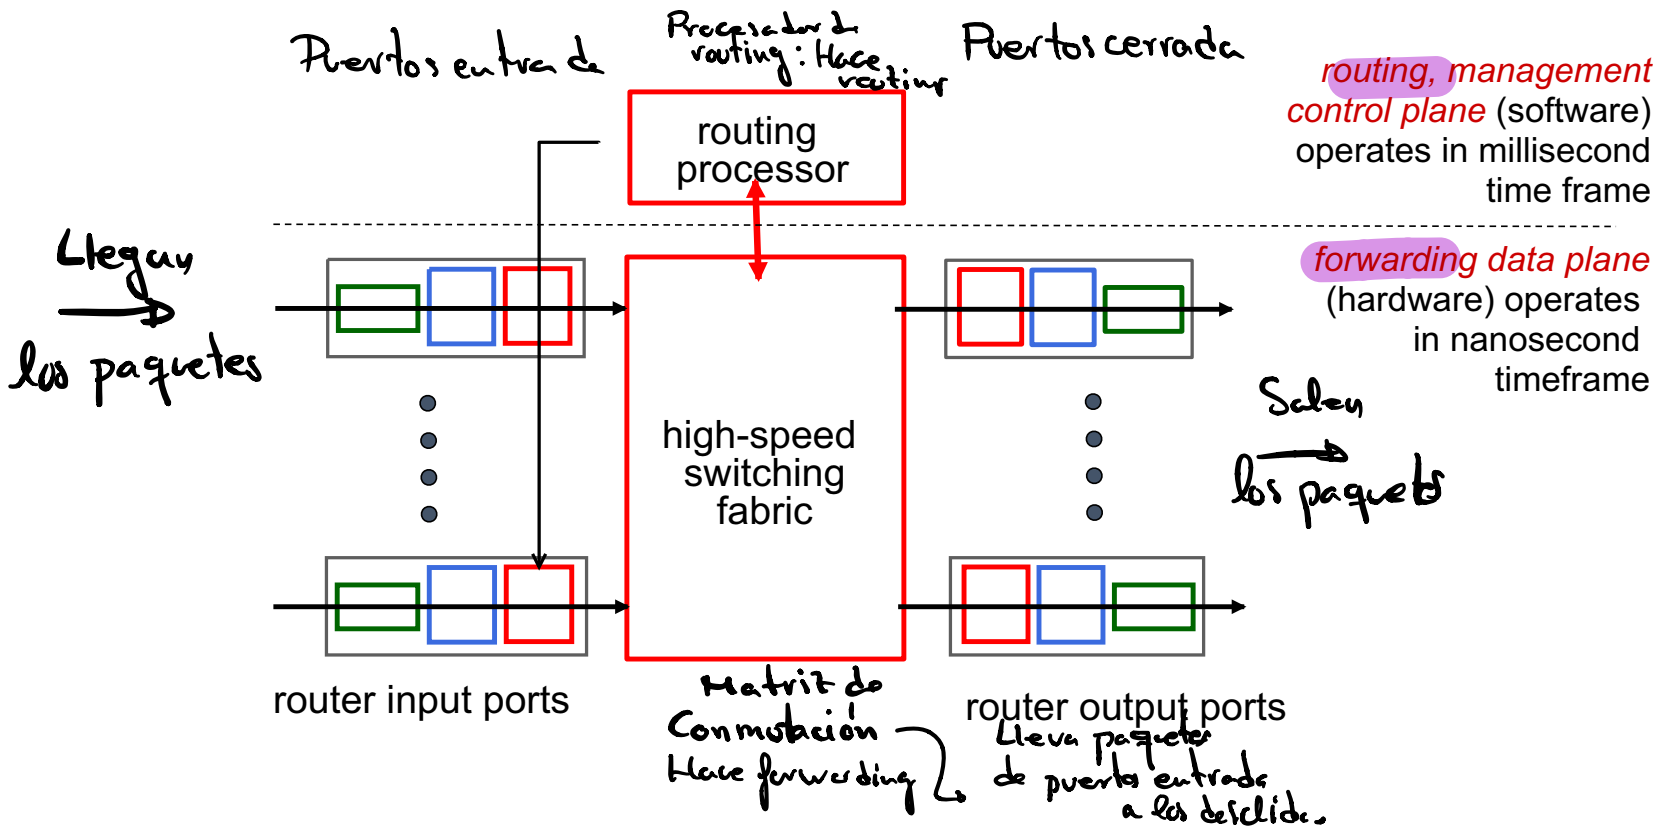
\includegraphics[scale=.25]{Untitled 22.png}}
\end{figure}
    Funciones del Puerto de entrada: 3 capas.
	\begin{figure}[H]
		\ffigbox[\FBwidth]
		{\caption{Puerto de entrada router}}
		{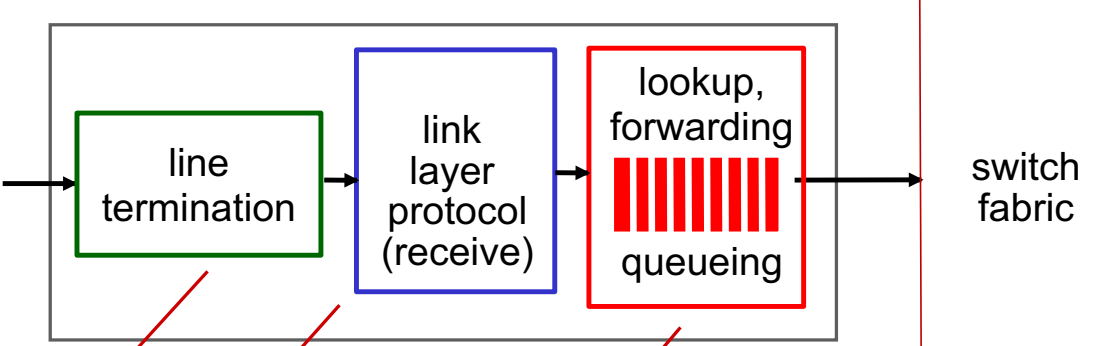
\includegraphics[scale=.25]{Untitled 23.png}}
	\end{figure}
    \begin{itemize}
    \item
      Física: Transforma los impulsos de luz a bits.
    \item
      Enlace: Procesa la capa de enlace.
    \item
      Tiene un buffer y la capacidad de hacer forwarding, es decir
      consultar el puerto de salida en las tablas de forwarding que nos
      indica a donde deben ir. El forwarding puede ser:

      \begin{itemize}
      \item
        Basado en el destino: Basado solo en la dirección IP destino.
      \item
        Generalizado: Basado en campos de la cabecera.
      \end{itemize}
    \end{itemize}
\pagebreak
	Matrices de conmutación: Permite hacer forwarding, lleva paquetes
    del puerto de entrada a los de salida adecuado.

    \begin{itemize}
    \item
      Tipos:

      \begin{itemize}
      \item
        De memoria: Bajo el control de la CPU, los paquetes se copian en
        memoria y la velocidad está limitada por el ancho de banda de
        memoria.
		\begin{figure}[H]
			\ffigbox[\FBwidth]
			{\caption{Matrices de conmutación de memoria}}
			{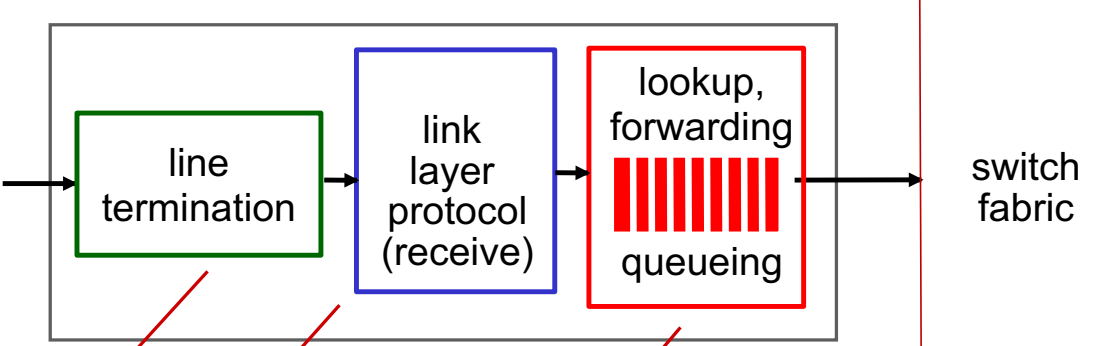
\includegraphics[scale=.15]{Untitled 23.png}}
		\end{figure}

        \begin{itemize}
        \item
          Llega un paquete a la entrada.
        \item
          Se pasa a memoria.
        \item
          Se determina la salida.
        \item
          Se saca el paquete de memoria y se lleva a la salida correcta.
        \end{itemize}
      \item
        De bus: Cada puerto tiene capacidad de memoria y procesamiento,
        y usa el bus para pasar de entrada a salida.
		\begin{figure}[H]
			\ffigbox[\FBwidth]
			{\caption{Matrices de conmutación de bus}}
			{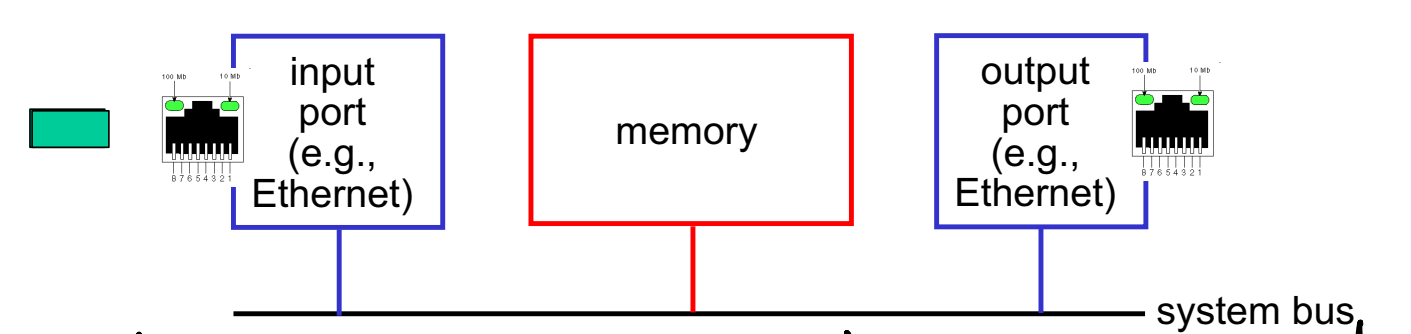
\includegraphics[scale=.15]{Untitled 24.png}}
		\end{figure}
        \begin{itemize}
        \item
          Hay limitación por el ancho de banda del bus.
        \item
          Para no saturar el bus: el ancho de banda del bus
          \textgreater= número de puertos de entrada*ancho de banda del
          puerto de entrada.
        \item
          Para no saturar la salida: ancho de banda de las entradas
          \textless= ancho de banda de las salidas
        \end{itemize}
      \item
        Red de interconexión: Caminos paralelos, todos conectados con
        todos, pero es caro tener una conexión entre cada uno.

        \begin{itemize}
        \item
          Para evitar que se haga tan caro, se usan múltiples planos
          para tener más caminos.
		  \begin{figure}[H]
			\ffigbox[\FBwidth]
			{\caption{Red de interconexión}}
			{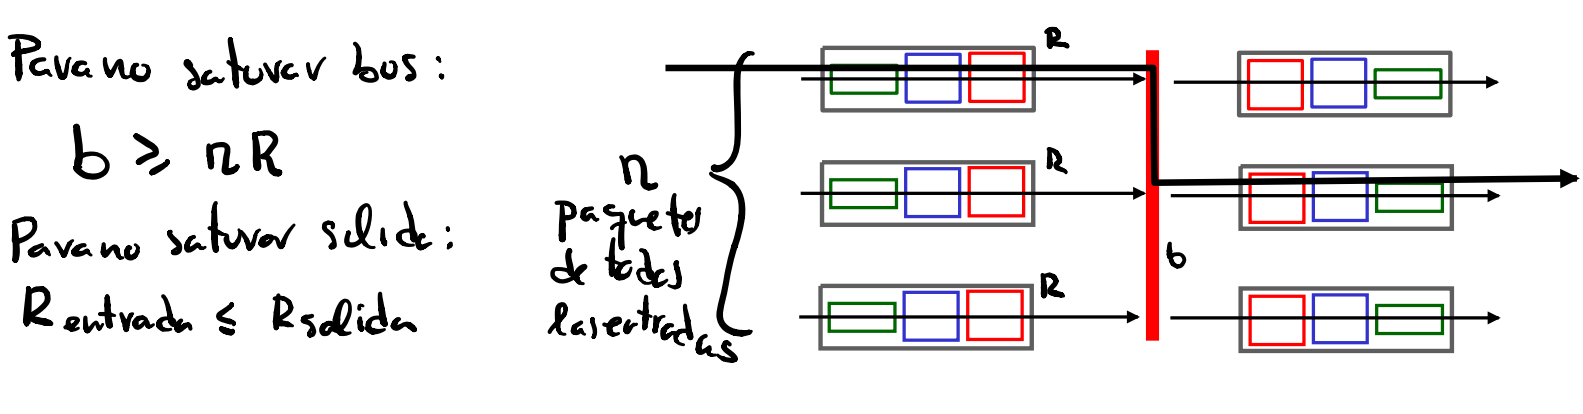
\includegraphics[scale=.2]{Untitled 25.png}}
		\end{figure}
        \end{itemize}

       
      \end{itemize}
    \end{itemize}
  
    Procesador de routing: Calcula la ruta, enruta.

	Puerto de salida: 3 etapas.

    \begin{itemize}
		\item
		Buffer sobre todo, para almacenar los paquetes que hay que sacar a
		la red que han llegado más rápido que la velocidad de transmisión.

		\begin{itemize}
		\item
			Administración del buffer: Hay una cola de paquetes, cuando se
			llena se pierden los que no entran o los de menor prioridad.
			Estrategias:

			\begin{itemize}
			\item
			FCFS - Primero en Llegar, Primero en Servir: En orden de
			llegada al puerto de salida.
			\item
			Prioridad: Puede haber dos o más colas, una de alta y otra de
			baja prioridad. Tipos:

			\begin{itemize}
			\item
				Primero se pasan los de alta prioridad y luego los otros.
			\item
				Cada n paquetes prioritarios, se cogen 1 no prioritario.
			\end{itemize}
			\item
			Round Robin: Varias colas y va rotando, se coge uno de cada
			cola.

			\begin{itemize}
			\item
				Se hace de forma equitativa y la prioridad la da un campo de
				la cabecera.
			\end{itemize}
			\item
			Weighted Fair Queueing -- Espera equitativa Ponderada: Como
			round robin, pero según el peso de cada cola, se cogen más o
			menos paquetes de esa cola en la rotación.
			\end{itemize}
		\end{itemize}
		\item
		Enlace.
		\item
		Física: Pasa bits a pulsos de luz.
    \end{itemize}
\pagebreak
\section{4.3 The Internet Protocol (IP): IPv4, Addressing, IPv6, and More}
\subsection{IP: Protocolo de Internet}

    Es un protocolo no confiable.

	Formato:
	\begin{figure}[H]
		\ffigbox[\FBwidth]
		{\caption{Diagrama mensaje IP}}
		{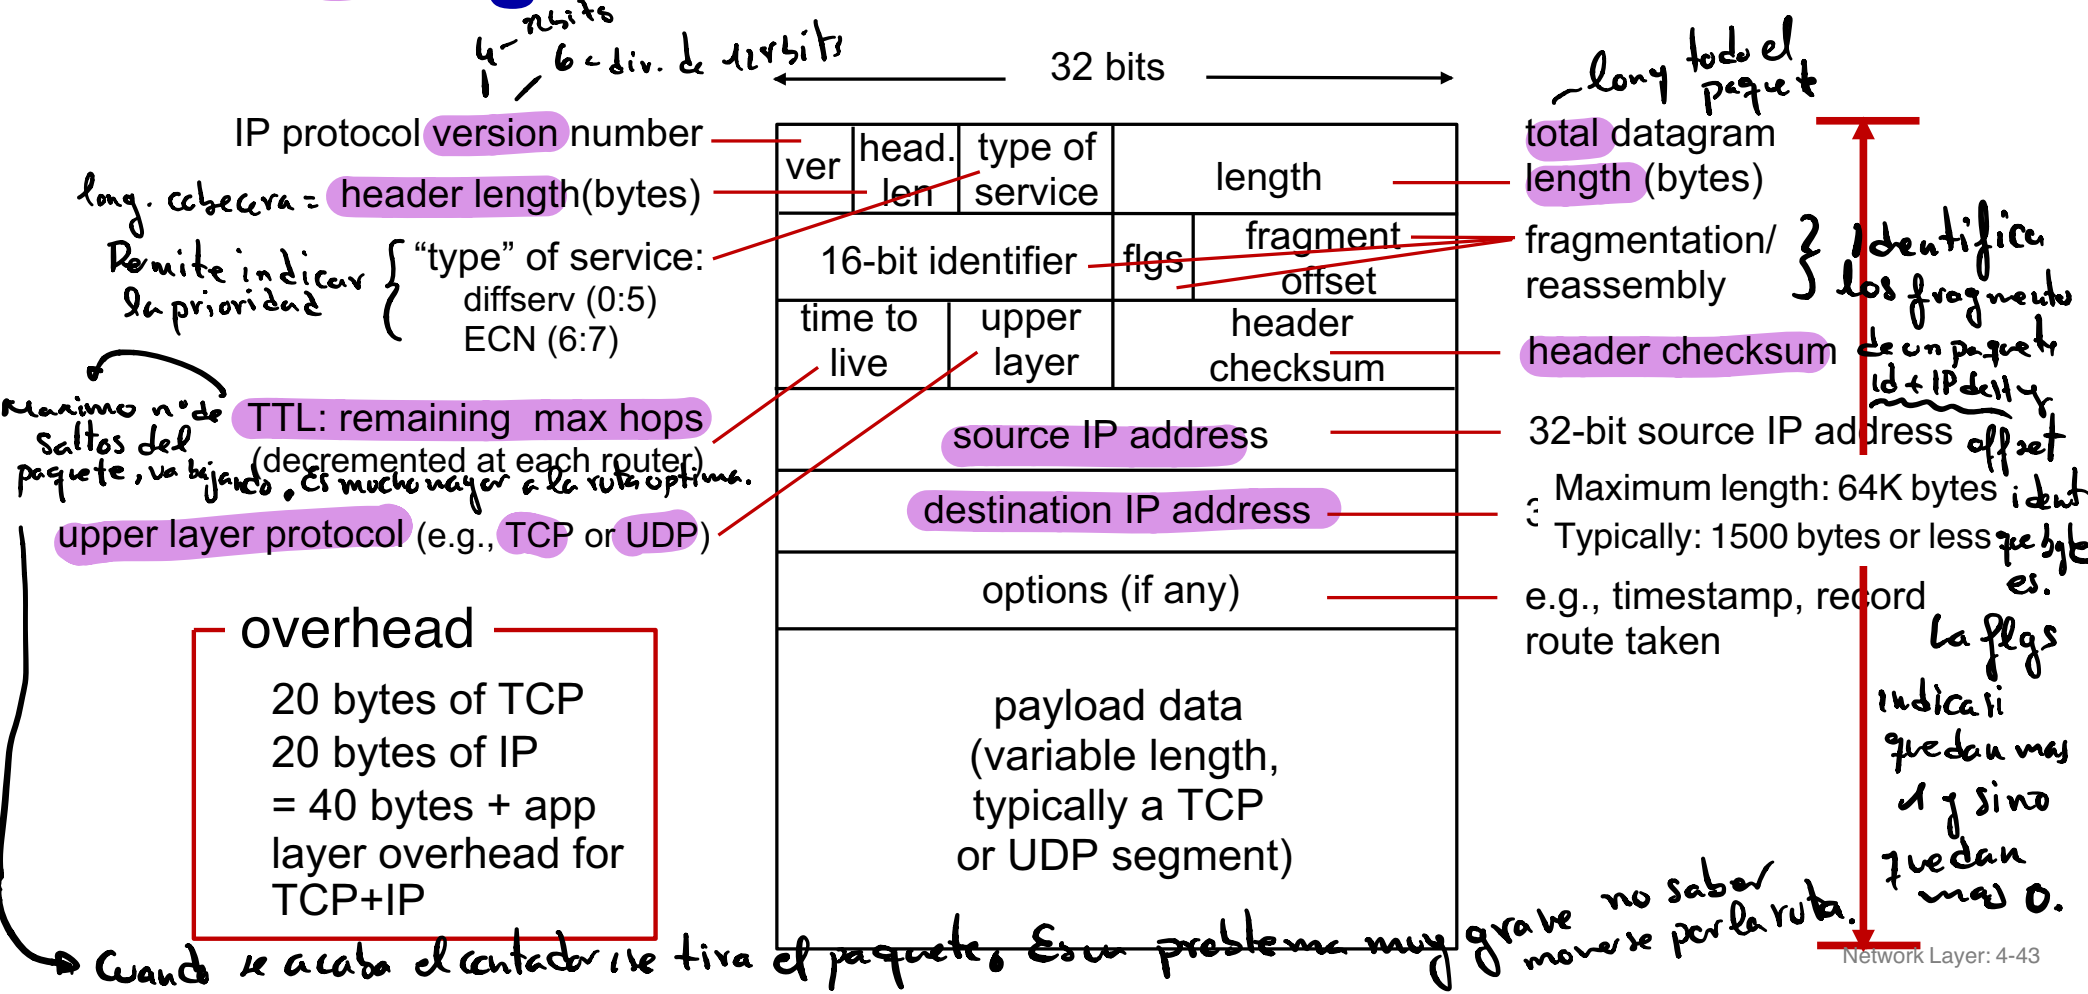
\includegraphics[scale=.17]{Untitled 28.png}}
	\end{figure}
    \begin{itemize}
    \item
      Cabecera: 20 bytes IP.

      \begin{itemize}
      \item
        Versión del protocolo: 4 32 bits y 6 128 bits.
      \item
        Longitud de la cabecera en bytes.
      \item
        Tipo de servicio: Permite indicar la prioridad.
      \item
        Longitud total del paquete.
      \item
        Identificar de 16 bits, flags y offset, para identificar los
        fragmentos de un mismo paquete al fragmentar.

        \begin{itemize}
        \item
          Id: Es fijo para el paquete.
        \item
          Flag: 1 si hay más fragmentos y 0 si es el último.
        \item
          Offset: Identifica el desplazamiento dentro del paquete
          fragmentado.
        \end{itemize}
      \item
        Tiempo de vida: máximo número de saltos de paquete, va bajando
        según salta. Es mucho mayor que los salto de la óptima. Si se
        acaba es un problema grave, ya que no es capaz de llevar los
        paquetes al destino.
      \item
        Protocolo de la capa superior: TCP o UDP.
      \item
        Checksum de la cabecera.
      \item
        IP origen.
      \item
        IP destino.
      \end{itemize}
    \item
      Segmento
    \end{itemize}

	Fragmentación y Reensamblado.

    \begin{itemize}
    \item
      Los enlaces tienen un máximo de tamaño de transferencia -- MTU.
    \item
      Los datagramas IP cuando son grandes, se fragmentan en la red (en
      cualquier dispositivo de la red) y cuando llega al destino se
      reensambla.
    \item
      Cada fragmento tiene en la cabecera un identificador que indica a
      que paquete corresponde y cuál es de todos.
    \item
      EJEMPLO:
	  \begin{figure}[H]
		\ffigbox[\FBwidth]
		{\caption{Ejemplo Fragmentación}}
		{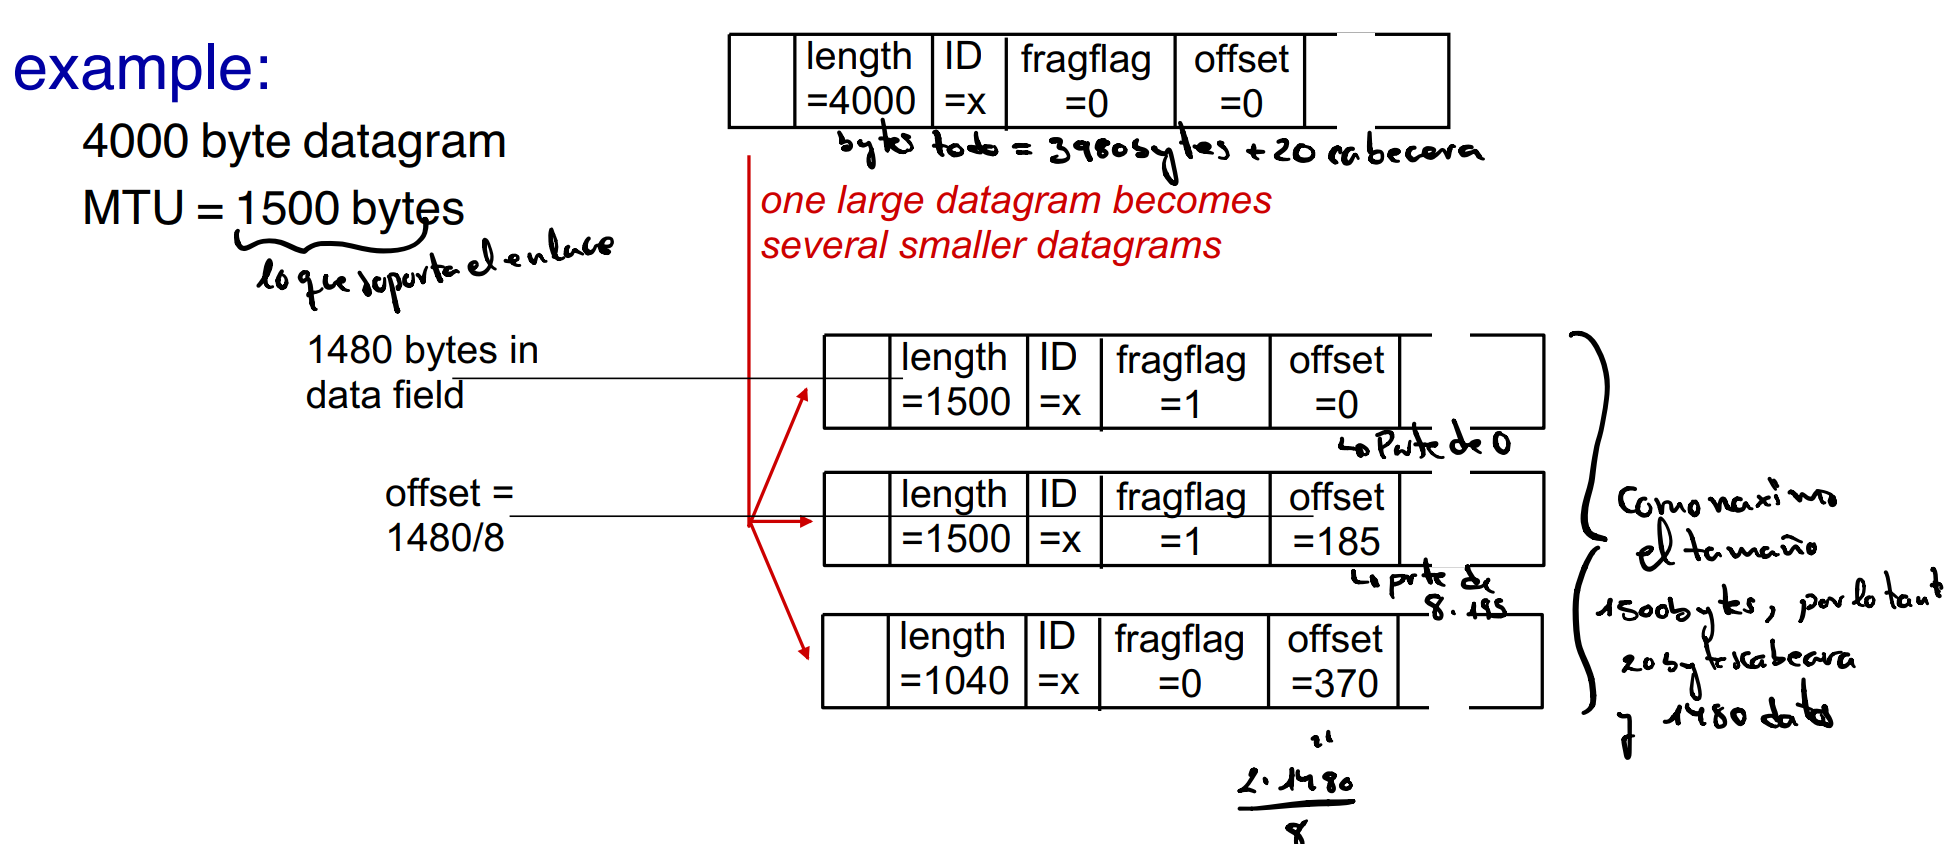
\includegraphics[scale=.21]{Untitled 29.png}}
	\end{figure}
    \end{itemize}

	\pagebreak
\subsection{Direccionamiento}


 
    EJEMPLO:
	\begin{figure}[H]
		\ffigbox[\FBwidth]
		{\caption{Ejemplo Direccionamiento}}
		{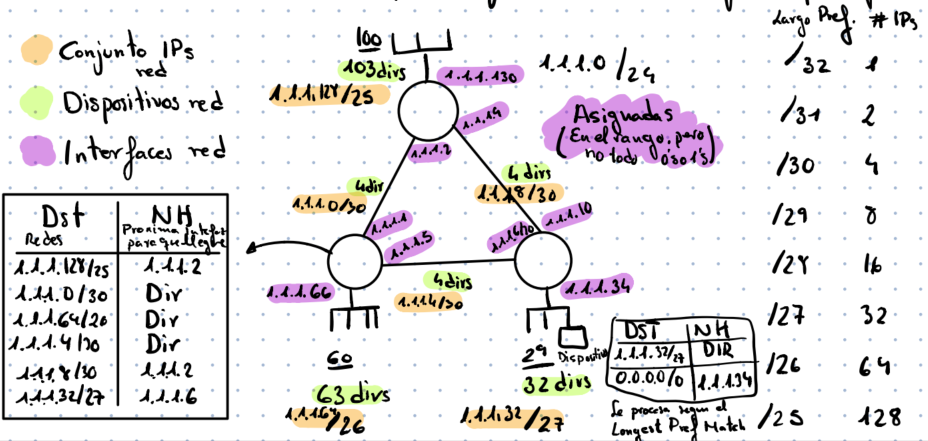
\includegraphics[scale=.3]{Untitled 30.png}}
	\end{figure}
    \begin{figure}[H]
		\ffigbox[\FBwidth]
		{\caption{Ejemplo Direccionamiento}}
		{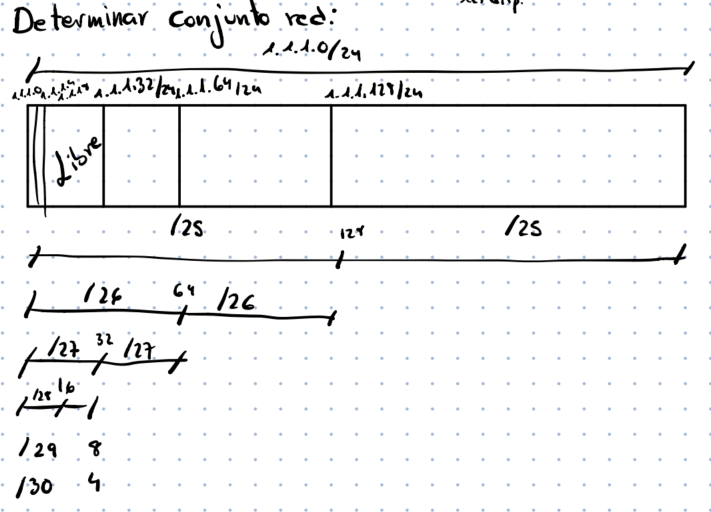
\includegraphics[scale=.3]{Untitled 31.png}}
	\end{figure}
  
    Pasos para asignar direcciones a una topología con subredes dadas:

    \begin{enumerate}
    \def\labelenumi{\arabic{enumi}.}
    \item
      Calcular el número de IP que necesita cada red,
      \#hosts+\#routers+1 de red+1 de broadcast
    \item
      Calcular el prefijo de cada red.

      \begin{itemize}
      \item
        /32 1, /31 2, /30 4, /29 8, /28 16, /27 32, /26 64, /25 128, /24
        255\ldots{}
      \end{itemize}
    \item
      Asignar IP con la tabla, dividiendo y viendo donde comienza cada
      bloque de IP.
    \end{enumerate}
  
    Maneras de obtener la dirección IP:

    \begin{itemize}
    \item
      Configurar el dispositivo manualmente.
    \item
      DHCP, se asignan de forma dinámica.
    \end{itemize}

	Necesitamos un espacio o sistema de nombres para identificar los
    elementos de la red con un nombre único.
  
    En internet se le asigna una dirección IP a cada interfaz.

    \begin{itemize}
    \item
      4 bytes separados por puntos, valores entre 0-255, en total 32
      bits.

      \begin{itemize}
      \item
        1.1.1.1= 00000001. 00000001.00000001.00000001
      \end{itemize}
    \item
      Hay \(2^{32}\) posibles valores, el tamaño máximo de internet.
    \item
      Cuando enviamos un paquete la IP se pone en la cabecera IP, para
      identificar al destinatario de forma única.
    \end{itemize}

	Tabla de Forwarding/reenvío:

    \begin{itemize}
    \item
      Columnas: Destino DEST y Siguiente salto NH (y Distancia, nos la
      dan o nos la inventamos y nos sirve para ordenar de menor a mayor
      distancia)
    \item
      En DEST se pone la IP de la red, es decir la de todo 0's con su
      prefijo.
    \item
      En NH:

      \begin{itemize}
      \item
        Si hay conexión directa, no se pone NADA, lo asigna el propio
        dispositivo.
      \item
        Si no es directa la conexión, se pone la dirección asignada a la
        entrada del router que lleva a esa red.

        \begin{itemize}
        \item
          Poner redundancia consiste en poner para el mismo DST varias
          direcciones de salto.
        \item
          Se pone la dirección de la red, la global, para todas las
          direcciones de las redes.
        \end{itemize}
      \end{itemize}
    \item
      Los DEST se ordenan de mayor a menor longitud de prefijo, y en
      caso de que haya varios con el mismo se ordenan entre ellos de
      menor a mayor distancia.
    \item
      La tabla de los dispositivos de una red es: Se pone la de la red y
      no se configura (vacía), y en la global de la red se pone la de
      salida.
	  \begin{figure}[H]
		\ffigbox[\FBwidth]
		{\caption{Tabla de Fordwarding}}
		{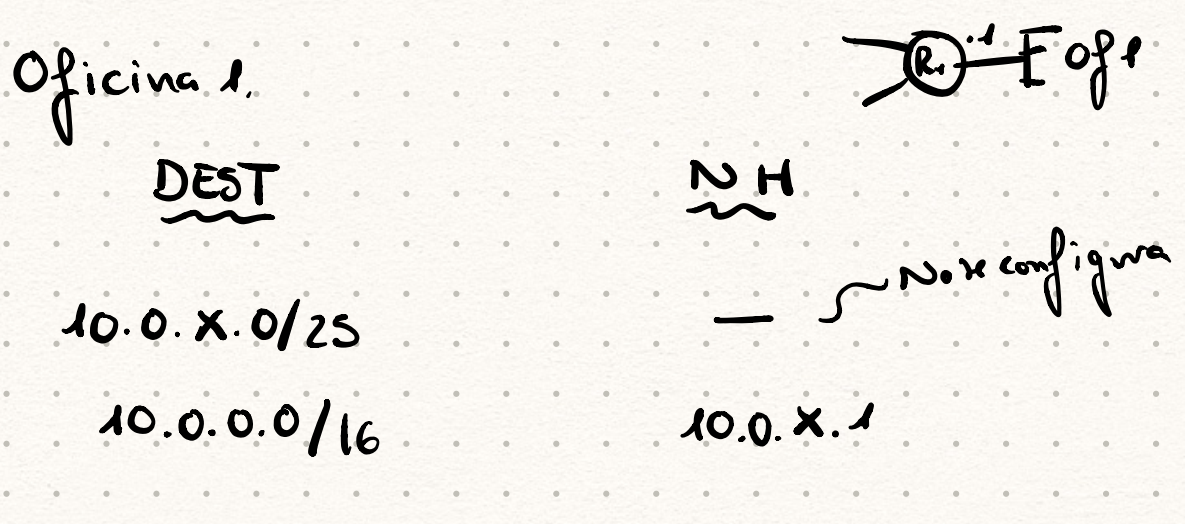
\includegraphics[scale=.2]{Untitled 32.png}}
	\end{figure}
    \end{itemize}

	Dos interfaces que no están en la misma red tendrán que usar al
    menos un router.

    \begin{itemize}
    \item
      Para ver el número de redes eliminamos los router y cada medio
      físico aislado es una red.
    \item
      En cada red necesitamos 1 para cada host, 1 para cada router, 1
      para la propia red todo 0's (la propia red) y 1 de broadcasts más
      todo 1's (referirnos a todos los dispositivos).

      \begin{itemize}
      \item
        \#dirs=\#hosts+\#routers+2
      \item
        60 dispositivos en una red=60+3= 63 direcciones IP necesita.
      \end{itemize}
    \end{itemize}

	En una red con 256 dirs. puede haber 254 routers y 253 si tiene que
    conectarse con el exterior.

	Enlace punto a punto: Conecta 1 a 1, no 1 a n o n a 1. No es un
    medio compartido.

	Cuando un paquete llega al router, se lee la cabecera IP, se extrae
    la dirección IP y se consulta la Tabla de forwarding (Contiene:
    Destino y Siguiente salto) donde indica según la IP que entrada debe
    tomar el paquete.

    \begin{itemize}
    \item
      No es factible que se almacene un valor para cada posible valor de
      IP, por tanto, se agrupan IP según la entrada.
    \item
      Todas las IP del conjunto tomarán la misma entrada y esos
      dispositivos deben tener una propiedad topológica para que envíe quien
      lo envié llegue.
    \end{itemize}

	CIDR - Classless InterDomain Routing: Porciones de la subred de
    longitud arbitraria
	\begin{figure}[H]
		\ffigbox[\FBwidth]
		{\caption{Classless InterDomain Routing}}
		{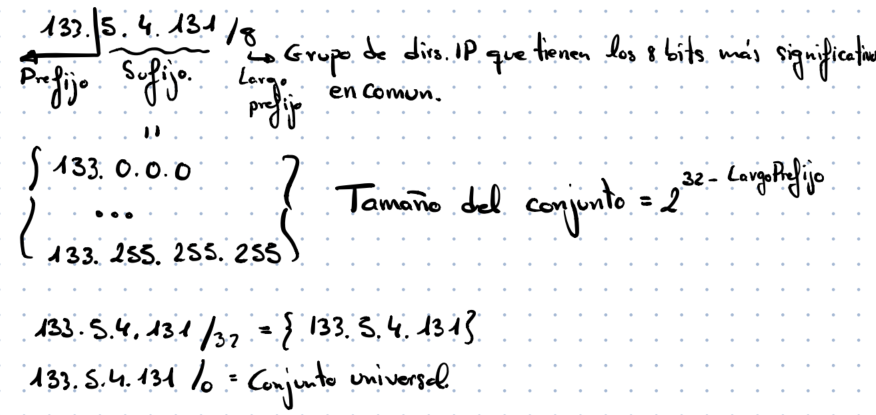
\includegraphics[scale=.4]{Untitled 34.png}}
	\end{figure}
	\begin{figure}[H]
		\ffigbox[\FBwidth]
		{\caption{Classless InterDomain Routing}}
		{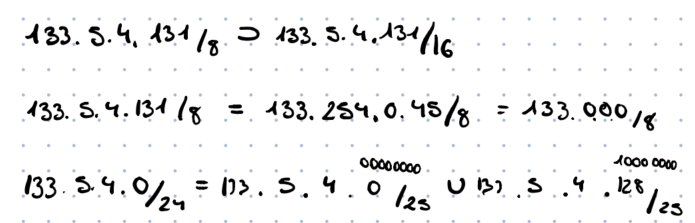
\includegraphics[scale=.5]{Untitled 35.png}}
	\end{figure}

	La IP se asigna a la interfaz del dispositivo, no al propio
    dispositivo.

    \begin{itemize}
    \item
      Un mismo dispositivo puede tener varias interfaces.
    \end{itemize}

	Red: Conjunto de interfaces conectadas por un medio físico.


	Hay que repartir las direcciones entre las distintas redes, cada red
  tiene su propio conjunto para las interfaces que lo forman.

  

\subsection{DHCP -- Dynamic Host Configuration
Protocol:}

  El host obtiene la dirección IP del servidor cuando entra en la red.

  Proceso:

  \begin{itemize}
  \item
    El host envía un mensaje a toda la red, para descubrir los DHCP
    server.
  \item
    Un DHCP recibe el mensaje, entonces ofrece al host una dirección IP.
  \item
    Recibimos esa dirección IP y se la confirmamos a DHCP.
  \item
    DHCP envía un asentimiento de que ha recibido la confirmación y nos
    la ha asignado.
  \end{itemize}

  No solo envía la dirección IP, también:

  \begin{itemize}
  \item
    La dirección del primer salto a router del cliente.
  \item
    Nombre y dirección del servidor DNS.
  \item
    La máscara de red.
  \end{itemize}

  La IP asignada es única en el sentido que no puede haber 2 usándola
  simultáneamente, pero en otro momento puede haber dispositivos que
  hayan usado la misma.

  Hay una jerarquía en la red, lo que permite que los cambios de IP se
  hagan de una forma más eficiente. Una parte importante figura son los
  ISP -- Internet Service Provider.

  ICANN -- Internet Corporation for Assigned Names and Numbers: Asigna
  los bloques de direcciones a los ISP, gestiona las DNS y dominios.

  \begin{itemize}
  \item
    Hay 5 registros regionales, distribuidos por el mundo.
  \item
    En 2011 asignaron el último bloque de direcciones IPv4.
  \item Gracias a NAT e IPv6 se solucionan las limitaciones de las IP.
  \end{itemize}


\subsection{NAT -- Network Address
Translation:}


  Para una misma red todos los dispositivos comparten la misma IPv4 a
  ojos del resto de internet.

  Cada dispositivo de la red se diferencia con un puerto, ya que tienen
  la misma IP entre ellos.

  Todos los dispositivos en la red local tienen una dirección de 32 bits
  en un espacio de direcciones privado (10/8, 172.16/12, 192.168/16
  prefijos) que solo puede ser usada en esa red.

  Ventajas:

  \begin{itemize}
  \item
    Con una sola IP, da servicio a todos los dispositivos del ISP.
  \item
    Cambiar la IP local no afecta fuera de la propia red.
  \item
    Cuando cambia la IP del ISP, no afecta a los dispositivos y su
    dirección privada.
  \item
    Es más seguro, no se puede direccionar un dispositivo directamente
    desde fuera de la red.
  \end{itemize}

  Implementación:

  \begin{itemize}
  \item
    Hace falta cambiar la dirección IP en los datagramas de salida y
    entrada a la IP de NAT, al igual que puertos.
  \item
    Hay una tabla de correspondencia de IP y puerto local -- IP y puerto
    NAT.
  \item
    Traduce IP y puerto local al de NAT y viceversa, mediante la Tabla
    de NAT.
  \end{itemize}
\pagebreak
  Controversia:

  \begin{itemize}
  \item
    Los routers deben solo procesar hasta el nivel 3, pero si alteran el
    puerto deben llegar a la 4.
  \item
    Cuando faltan direcciones se deben usar las direcciones IPv6, en vez
    de NAT.
  \item
    Los extremos son los únicos que deben poder alterar los puertos.
  \end{itemize}

  A pesar de los inconvenientes se usa NAT en muchos ámbitos.

  
\subsection{IPv6:}



  Surge de la limitación de 32 bits de IPv4, ya que actualmente hay
  mucha variedad de dispositivos con su propia IP.

  Se pasa de 32 a 128 bits.

  Además:

  \begin{itemize}
  \item
    Mejora la velocidad de enviado y procesado. Protocolo más eficiente.
    Para ello opta por una cabecera fija de 40 bytes.
  \item
    Permite tratar los flows en distintas capas. Esto mejora el
    tratamiento de la comunicación de las aplicaciones de tiempo real.
  \end{itemize}

  Formato del datagrama:
  \begin{figure}[H]
	\ffigbox[\FBwidth]
	{\caption{Formato del datagrama IPv6}}
	{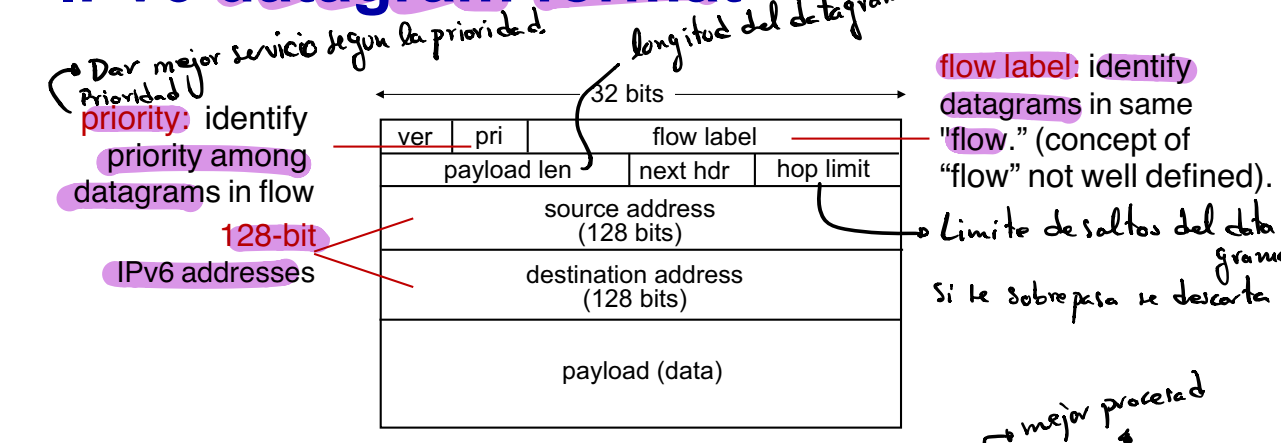
\includegraphics[scale=.3]{Untitled 36.png}}
\end{figure}
\pagebreak
  \begin{itemize}
  \item
    Cabecera

    \begin{itemize}
    \item
      Versión del protocolo.
    \item
      Prioridad, dar mejor servicio según la prioridad.
    \item
      Etiqueta de Flow, identifica los datagramas dentro del Flow.
    \item
      Longitud del datagrama completo.
    \item
      Next hdr.
    \item
      Límite de saltos del datagrama, si se sobrepasa se descarta.
    \item
      Dirección IPv6 origen.
    \item
      Dirección IPv6 destino.
    \end{itemize}
  \item
    Datos -- payload
  \item
    No tiene: Checksum, fragmentación y reensamblado y tampoco opciones
    extra.
\end{itemize}

	Transición

    \begin{itemize}
    \item
      Conviven ambos protocolos gracias al tunneling.
    \item
      No todos los dispositivos pueden hacer esta mejora.

      \begin{itemize}
      \item
        El 30\% de los clientes acceden a Google de esta manera.
      \item
        1/3 de los dominios del gobierno de los estados unidos son
        capaces.
      \end{itemize}
    \item
      Se han tardado 25 años hasta este punto, pero todavía queda.
  \item
    Tunneling:
	\begin{figure}[H]
		\ffigbox[\FBwidth]
		{\caption{Tunneling}}
		{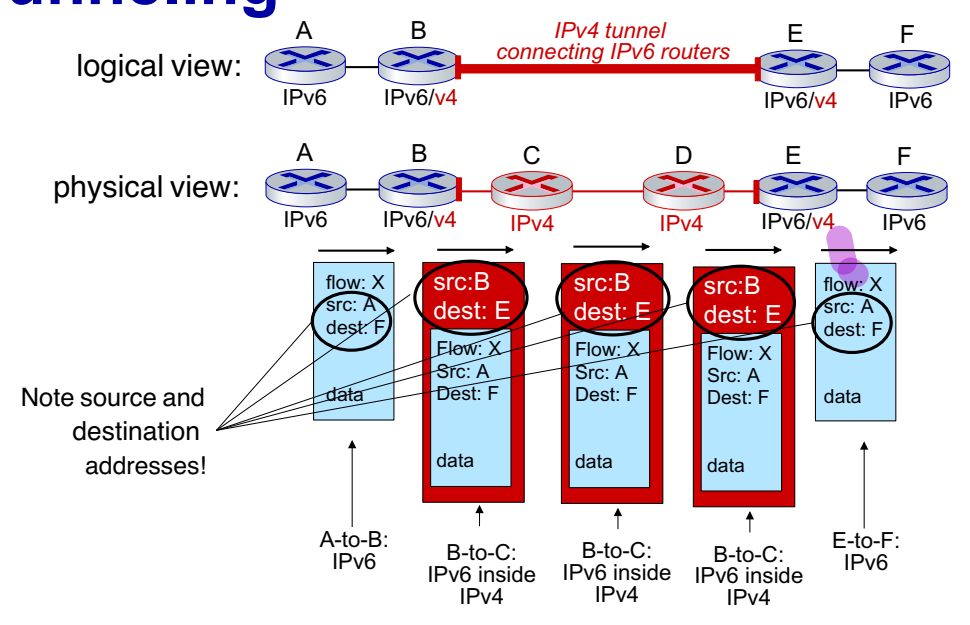
\includegraphics[scale=.3]{Untitled 37.png}}
	\end{figure}
    \begin{itemize}
    \item
      Los datagramas de IPv6 se encapsulan en datagramas de tipo IPv4
      como datos, para ser gestionado por los dispositivos que admiten
      solo IPv4.
    \item
      Se crea un túnel por los routers de versión 4 indicando hasta
      donde mantenerlo, y cuando se pasa se deshace el encapsulado y se
      sigue pasando IPv6.
    \end{itemize}
	\end{itemize}

	El protocolo IP es la única de su capa, a diferencia del resto de
    capas que tienen muchas alternativas. IP debe estar implementada en
    todos los dispositivos.
	\begin{itemize}
  \item
    A veces se necesitan otros elementos para resolver ciertos problemas
    de IP, como NAT o Firewalls. Ya sea por limitación de direcciones o
    la mejora de la eficiencia.
  \end{itemize}

\subsection{Principio arquitectónico de Internet:}

  \begin{itemize}
  \item
    El objetivo de internet, era la conectividad, mediante el Internet
    Protocol y la gestión/inteligencia se hará en los extremos y no
    oculta en la red.
  \item
    El end-end argument: Dice que la complejidad o lógica de la
    conectividad se puede implementar en los extremos en vez de
    soportarla la red.
  \item
    Se puede ver en la capa de protocolos, los extremos hacen la
    comunicación y la red se queda en las 3 primeras.
  \item
    Aunque algunas funcionalidades pueden implementarse en la red, como
    congestión o transferencia fiable.

	\begin{figure}[H]
		\ffigbox[\FBwidth]
		{\caption{Principio arquitectónico de Internet}}
		{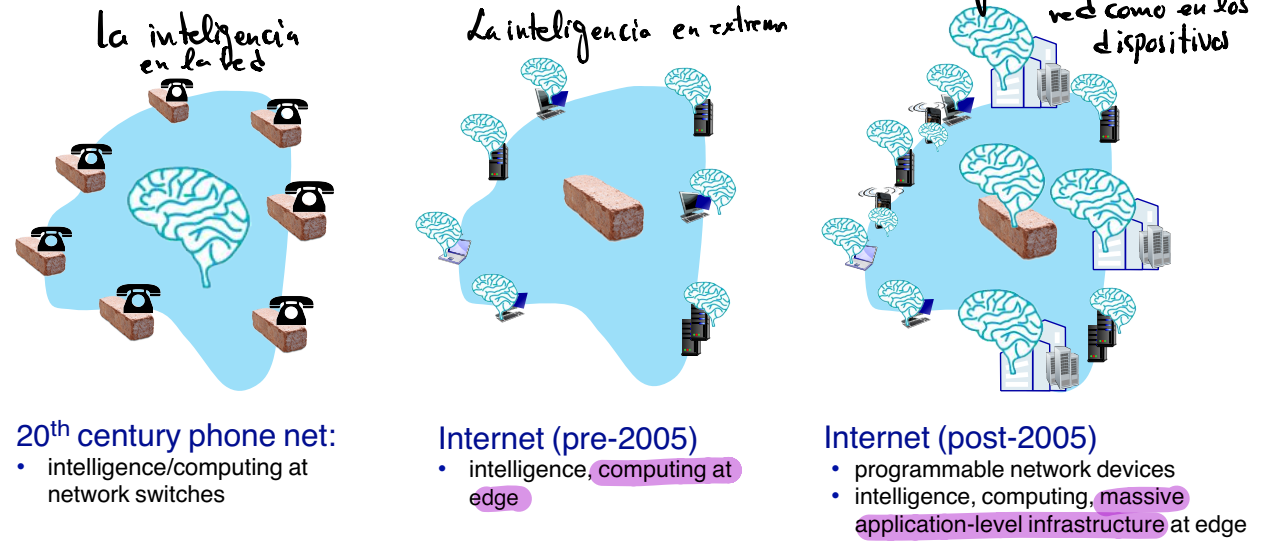
\includegraphics[scale=.35]{Untitled 38.png}}
	\end{figure}
  \item
    ICMP -- Internet Control Message Protocol: Protocolo que utilizan
    los dispositivos con los routers y viceversa para comunicar
    información a nivel de red, ya sean errores o llegadas de datos
    (ping).

    \begin{itemize}
    \item
      Contenido del mensaje: Tipo, código y los 8 primeros bytes del
      datagrama IP que causa el error.
    \item
      Relación con Traceroute:

      \begin{itemize}
      \item
        Envía 3 paquetes por iteración, según progresan las iteraciones
        se va aumentando su tiempo de vida.
      \item
        Cuando se termina el tiempo se recibe error de que no llega, TTL
        expired, que también informa en que IP y router se ha terminado.
        Vuelve a mandando paquetes como más tiempo de vida.
      \item
        Cuando llega al destino, port unreachable, conocemos la ruta
        tomada.
      \end{itemize}
    \end{itemize}
  \end{itemize}

\chapter{TEMA 5: Network Layer Control Plane}

\section{5.1 Introduction}

 

    La función del plano de control es determinar el camino que deben
    seguir los paquetes desde el origen hasta la salida.

	A diferencia que el plano de datos que es elegir la salida apropiada
    del router.

	Dos aproximaciones:

    \begin{itemize}
		\item
		Per-router: Configurar cada router/dispositivo manualmente.
		\begin{figure}[H]
			\ffigbox[\FBwidth]
			{\caption{Per-router}}
			{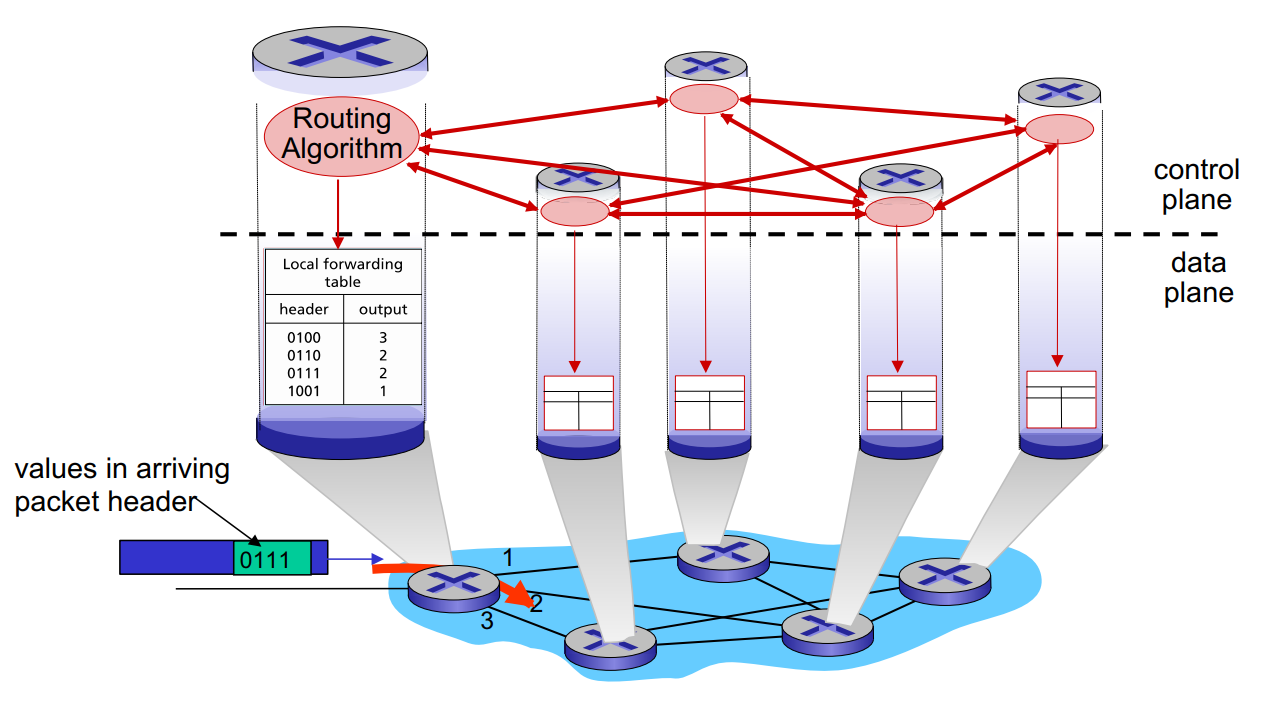
\includegraphics[scale=.3]{Untitled 20.png}}
		\end{figure}
		\begin{itemize}
		\item
			Todo y cada uno de los router tiene un algoritmo de enrutado,
			que le configura las tablas de ruta.
		\end{itemize}
		\pagebreak
		\item
		SDN -- Software Defined Networking: Todo el enrutado se hace
		mediante software desde un punto centralizado.
		\begin{figure}[H]
			\ffigbox[\FBwidth]
			{\caption{Software Defined Networking}}
			{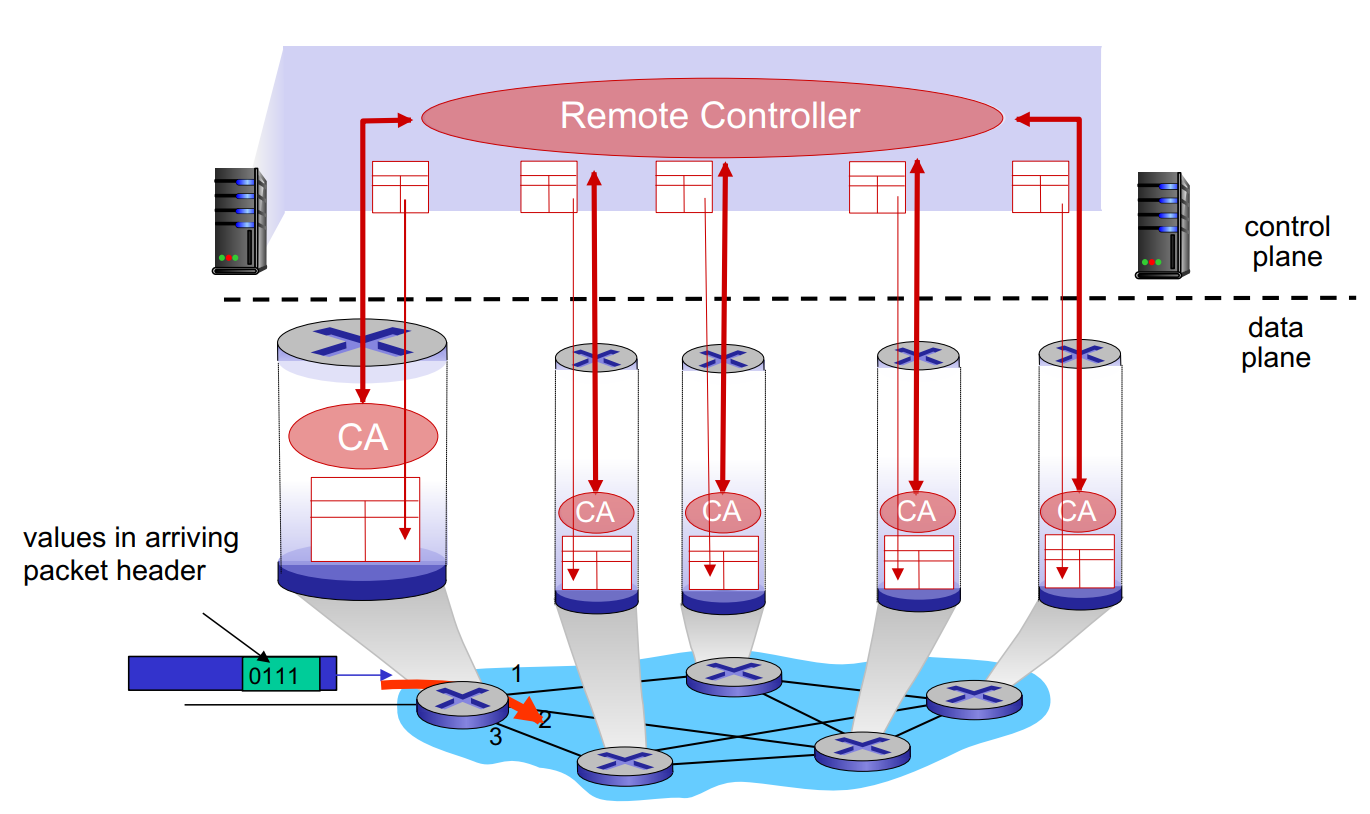
\includegraphics[scale=.3]{Untitled 21.png}}
		\end{figure}
		\begin{itemize}
		\item
			Hay un controlador remoto que configura las tablas de los
			routers, un proceso centralizado que se comunica con todos los
			routers.
		\end{itemize}
    \end{itemize}

	
\section{5.2 Routing Algorithms}

    Protocolos de enrutamiento: Tratan de buscar el mejor camino en
    comunicaciones host to host, de punto a punto.

    \begin{itemize}
    \item
      Camino: Secuencia de routers que deben atravesar los paquetes
      desde el host inicial dado el host destino.
    \item
      Se puede buscar la mejor, pero con respecto a varios parámetros
      como coste, rapidez o menos congestión.
    \end{itemize}

	Se representan en forma de grafo:

    \begin{itemize}
    \item
      Los vértices son los routers.
    \item
      Los arcos son los enlaces entre routers.
    \item
      Los costes de los arcos son el coste en atravesarlo de un punto a
      otro. Viene dado por el operador de red. Los conectados
      directamente tienen un valor, si no es infinito el coste entre
      ambos.
    \end{itemize}

	Clasificación de los algoritmos de routing: Dos planos, global o
    descentralizada y estática o dinámica.

    \begin{itemize}
    \item
      Global: Todos los routers tienen completa información sobre la
      topología y costes de enlace.

      \begin{itemize}
      \item
        Algoritmo de estado de enlace.
      \end{itemize}
    \item
      Descentralizada: La información está distribuida, cada router solo
      conoce el estado y costes de sus vecinos físicamente conectados.
      Es un proceso iterativo de computación e intercambio de
      información con los vecinos.

      \begin{itemize}
      \item
        Algoritmo de vector de distancias.
      \end{itemize}
    \item
      Estática: Las rutas cambian poco en el tiempo.
    \item
      Dinámica: Las rutas cambian rápidamente, actualización periódica
      en respuesta a cambios en el coste de enlaces.
    \end{itemize}

	Algoritmo estado de enlaces -- link state: Algoritmo de enrutado
    estado de enlaces de Dijkstra.

    \begin{itemize}
    \item
      Centralizado: Tiene información completa sobre todos los nodos de
      la red.
    \item
      Calcula la ruta de menor coste desde ese nodo al resto de nodos,
      proporciona la tabla de enrutamiento de ese nodo.
    \item
      Es iterativo, después de k iteraciones conoce los caminos de menor
      coste.
    \item
      Notación:

      \begin{itemize}
      \item
        \(c_{x,y}\): Coste de los enlaces directos, si no los hay
        infinito.
      \item
        \(D(v)\): Estimación actual del coste hasta v.
      \item
        \(p(v)\): Nodo anterior a v en la ruta.
      \item
        \(N’\): Conjunto de nodos de los que se conoce el camino de
        menor coste, van entrando los menos del algoritmo.
      \end{itemize}
	  \pagebreak
    \item
      Algoritmo:
	  \begin{figure}[H]
		\ffigbox[\FBwidth]
		{\caption{Algoritmo de Dijsktra}}
		{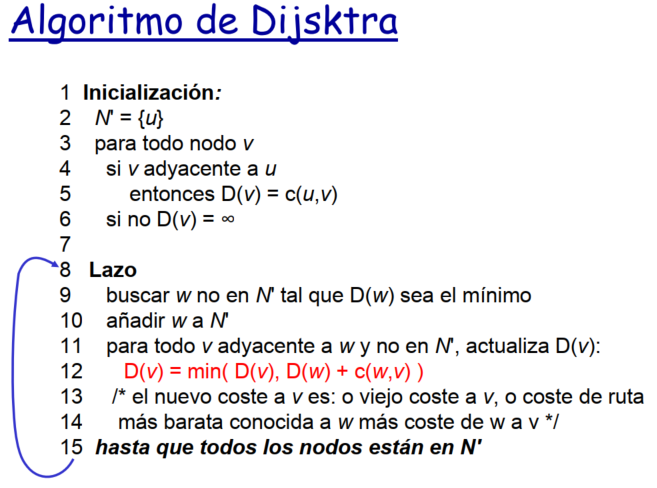
\includegraphics[scale=.4]{Untitled 39.png}}
	\end{figure}
    \item
      La complejidad del algoritmo es \(O(n^2)\), una mejor
      implementación tendrá \(O(n \log (n))\)
    \item
      La complejidad de mensaje, cada router debe transmitir la
      información de estado a los n routers
    \item
      Posibles oscilación/fluctuaciones de ruta, según la cantidad de
      tráfico en los enlaces, lo que hace que tenga que recomputar todas
      las rutas.
    \item
      Ejemplo:
	  \begin{figure}[H]
		\ffigbox[\FBwidth]
		{\caption{Algoritmo estado de enlaces}}
		{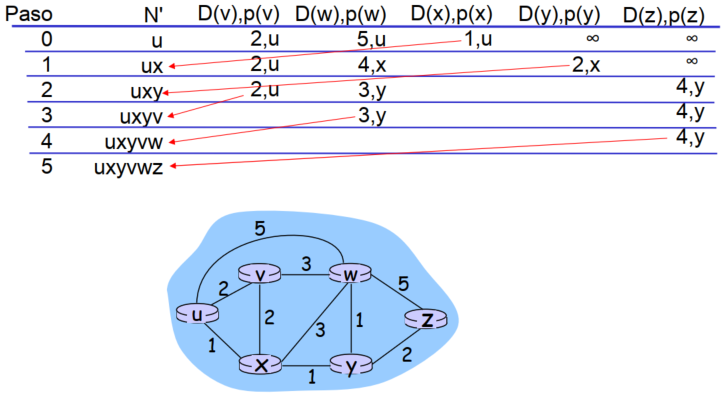
\includegraphics[scale=.35]{Untitled 40.png}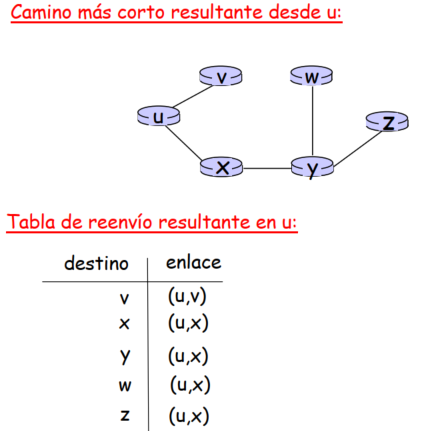
\includegraphics[scale=.35]{Untitled 41.png}}
	\end{figure}

    \end{itemize}
\pagebreak
	Algoritmo vector de distancias -- distance vector: Basado en la
    ecuación de Bellman-Ford.

    \begin{itemize}
    \item
      \(D_x(y)\): Coste del camino más barato desde x a y
    \item
      \(D_c(y)=min_v \{ c_{c,v}+D_v(y)\}\) El mínimo se toma sobre todos
      los vecinos v de x.

      \begin{itemize}
      \item
        Calcula la ruta de menor cote de un nodo x a un nodo y, será el
        mínimo para todo vecino de ir al vértice más el menor coste
        desde ese vértice hasta y.
      \end{itemize}
	  \item
    Algoritmo
	\begin{figure}[H]
		\ffigbox[\FBwidth]
		{\caption{Algoritmo vector de distancias I}}
		{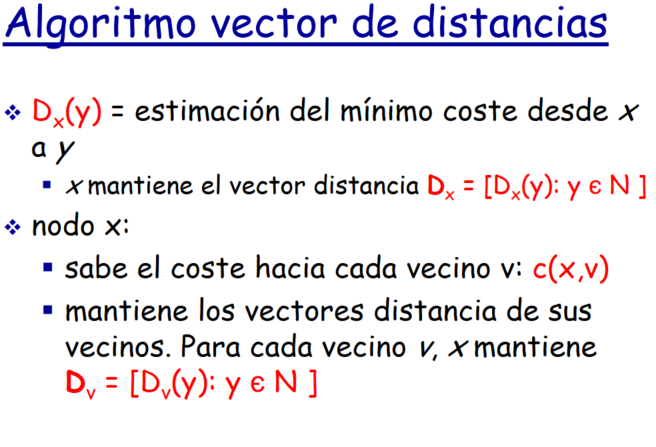
\includegraphics[scale=.35]{Untitled 42.png}}
	\end{figure}
    \begin{itemize}
    \item
      La clave es que cada nodo envía su vector de distancia solo a sus
      vecinos, cuando recibe el de los vecinos actualizas tu vector de
      distancia y lo vuelves a mandar.
    \item
      Iterativo, asíncrono: Una iteración local viene causada por

      \begin{itemize}
      \item
        El cambio de coste en el enlace local
      \end{itemize}
    \item
      Mensaje de actualización de DV desde un vecino.
	  \begin{figure}[H]
		\ffigbox[\FBwidth]
		{\caption{Algoritmo vector de distancias II}}
		{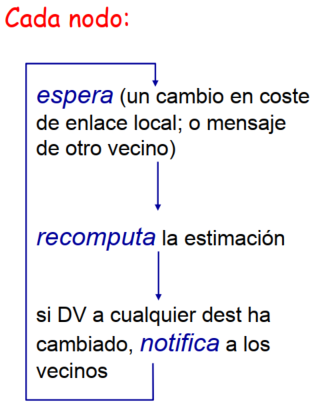
\includegraphics[scale=.4]{Untitled 43.png}}
	\end{figure}
    \item
      Distribuido: cada nodo notifica a los vecinos solo si su propio DV
      cambia, y los vecinos a sus vecinos, si es necesario.
    \item
      Cada iteración va llegando a datos de más lejos, se propaga, y
      teniendo en cuanto más caminos.
    \item
      Los cambios se hacen de forma asimétrica, lo que hace que cambien
      más rápido los costes.

      \begin{itemize}
      \item
        Bad news travel slow, cuesta superar los costes al escoger los
        mínimos.
      \item
        Good news travel fast, se superan antes al ser menores.
      \end{itemize}
    \end{itemize}
  \item
    Ejemplo
	\begin{figure}[H]
		\ffigbox[\FBwidth]
		{\caption{Ej. vector de distancias}}
		{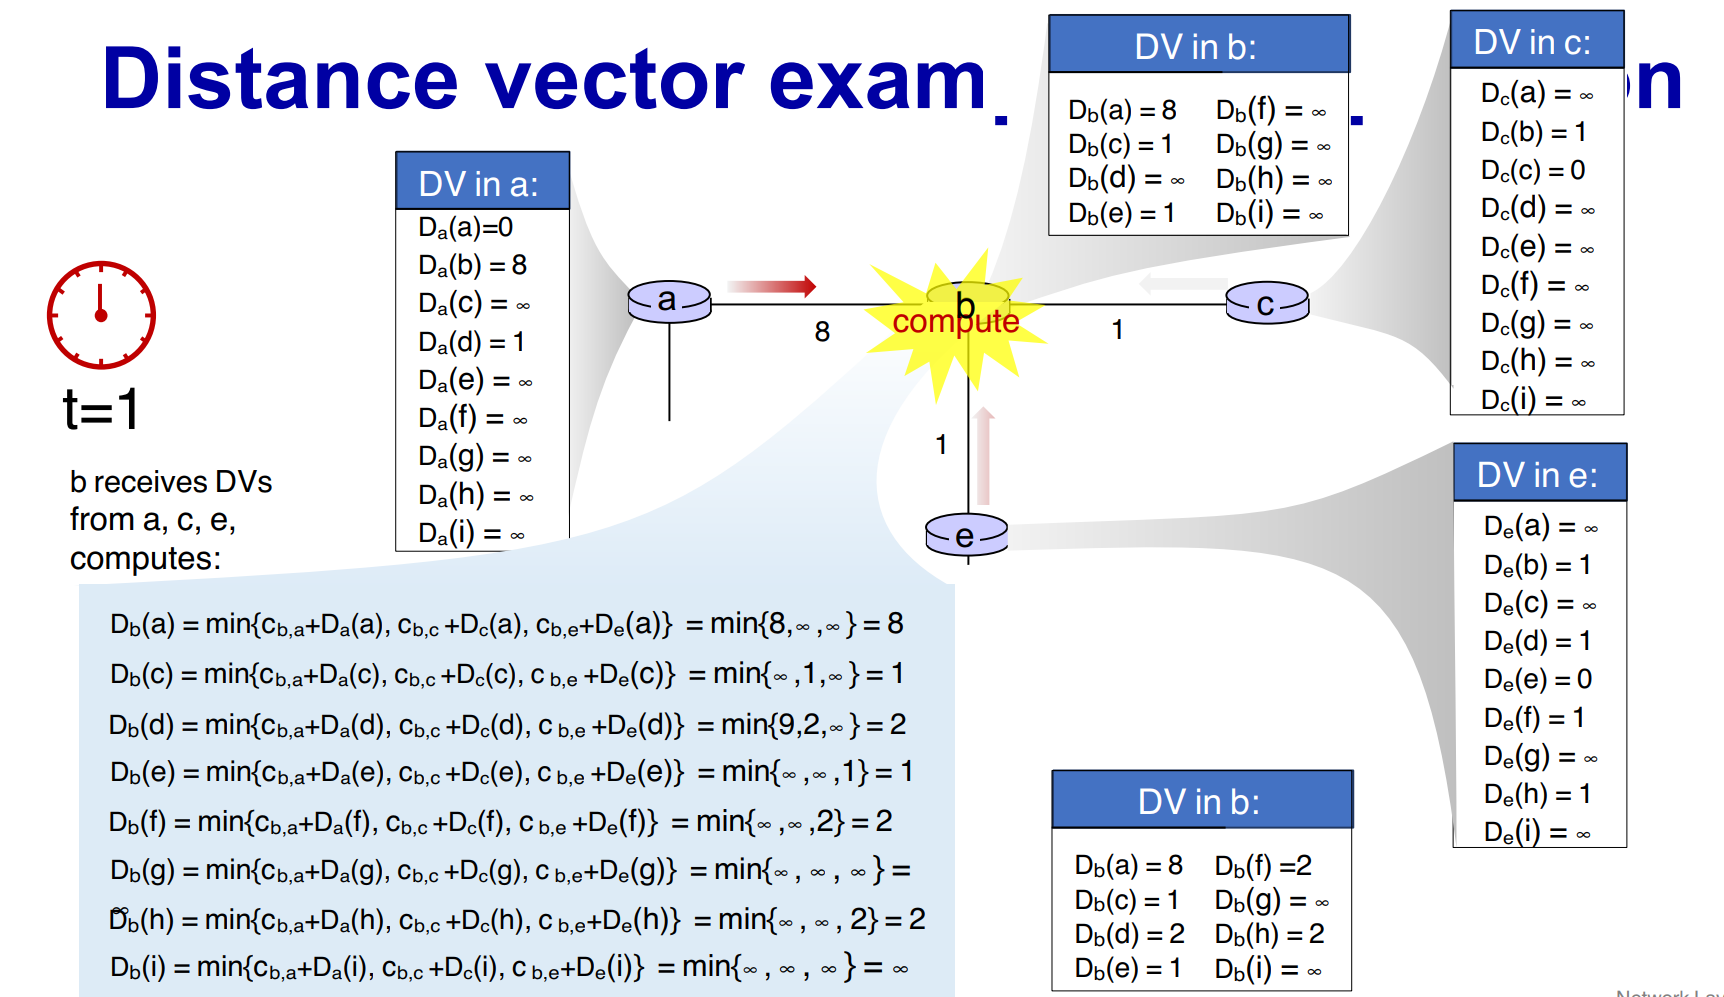
\includegraphics[scale=.25]{Untitled 44.png}}
	\end{figure}
    \end{itemize}
  

	Comparación de estado de enlaces y vector de distancias:

    \begin{itemize}
    \item
      Complejidad del mensaje:

      \begin{itemize}
      \item
        LS: Con n nodos, E enlaces, se envían \(O(nE)\) mensajes.
      \item
        DV: Intercambio solo entre vecinos.
      \end{itemize}
    \item
      Complejidad de la convergencia:

      \begin{itemize}
      \item
        LS: Algoritmo \(O(n^2)\), necesita \(O(nE)\) enlaces.
      \item
        DV: Tiempo de convergencia variable.
      \end{itemize}
	  \pagebreak
    \item
      Robustez:

      \begin{itemize}
      \item
        LS: El nodo puede difundir un coste de enlace erróneo, cada nodo
        computa solo su propia tabla no se propaga.
      \item
        DV: El nodo DV puede difundir un coste de ruta erróneo, se
        propagaría por la red al pasarlo a los vecinos.
      \end{itemize}
    \end{itemize}

	Enrutamiento jerárquico:

    \begin{itemize}
    \item
      Hasta ahora hemos estudiado un modelo idealizado, todos los
      routers idénticos y una red plana, pero no es así en la práctica.
    \item
      Escala: Hay tantos destinos que no se puede tener una tabla de
      routing con todos ellos, la tabla sería tan grande que saturaría
      los enlaces.
    \item
      Autonomía administrativa: Cada administrador de red querrá
      controlar su propia porción de la red.
    \item
      Sistemas Autónomos o dominios -- AS: agregación/agrupación de
      routers en regiones.
    \item
      Intra-AS -- Intradominios: Enrutado dentro del mismo dominio.

      \begin{itemize}
      \item
        Routers en el mismo AS ejecutan el mismo protocolo de
        enrutamiento.
      \item
        Routers en diferente AS pueden ejecutar diferentes protocolos
        intra-AS.
      \item
        Gateway router -- Router pasarela: Están en la frontera de su
        AS. Enlaza con otros routers pasarela.
      \end{itemize}
    \item
      Inter-AS -- Interdominio: Enrutado entre dominios.

      \begin{itemize}
      \item
        Los router pasarela hacen el enrutamiento entre dominios.
      \end{itemize}
    \end{itemize}

	La tabla de reenvío se configura tanto con algoritmos intra-AS como
    inter-dominio.

    \begin{itemize}
    \item
      Entradas intra-AS para destinos internos.
    \item
      Entradas inter-AS e intra-AS para destinos externos.
    \end{itemize}

	Los router de un dominio deben conocer que destinos tienen los
    dominios vecinos para saber a qué router pasarela hay que enviar los
    datagramas, esos datos los proporciona el routing inter-AS.

\pagebreak	
\section{5.3 Intra-AS Routing in the Internet: OSPF}

    Protocolos intradominio más comunes, llamados IGP -- Interior
    Gateway Protocols:

   
	\subsection{RIP -- Routing Information Protocol (incluido en la distribución BSD-UNIX en 1982)}

      \begin{itemize}
      \item
        Basado en vector de distancia.

        \begin{itemize}
        \item
          Permite un máximo de 15 saltos, cada enlace cuesta 1.
        \item
          Intercambia con los routers vecinos cada 30 segundos, llamado
          anuncio RIP.
        \item
          En cada anuncio, lista de hasta 25 subredes destino, en
          sentido IP.
        \end{itemize}
      \item
        Fallo y recuperación de enlace:

        \begin{itemize}
        \item
          Si tras 180 segundo no recibe anuncio de un vecino, entiende
          que el vecino o el enlace han muerto.
        \item
          Invalida rutas a través de muerto.
        \item
          Envía anuncios a los demás vecinos, y estos si actualizan su
          vector enviaran la suya.
        \item
          Si muere la información se propaga rápido.
        \item
          Inversa envenenada: Se usa para evitar bucles ping-pong, se
          considera distancia infinita 16 saltos, ya que supera el
          límite de saltos.

          \begin{itemize}
          \item
            En la práctica se pone valor infinito por el que debe pasar,
            de esta manera este no tratara de pasar por él, y al resto
            les informa del valor real (el coste desde ese nodo al
            destino)
          \item
            Si se corta un enlace con un router, informara de coste
            infinito (16) a los vecinos de esta manera tardaran menos en
            actualizar los costes.
          \end{itemize}
        \item
          Cuenta hasta infinito: Cuando cambia el coste de un enlace
          provocando que se tarden infinito o muchos ciclos en
          estabilizar, ya que el que se encuentra directamente afectado
          por ese aumento tratara de llegar por otro lado, pero lo que
          no sabe es que ese lado le utilizaba a él para llegar y se
          hace un bucle de actualizaciones. Una solución es suponer que
          una vez que la distancia es 16 es infinito, de esta manera
          para de calcular la distancia hacia ese nodo.
        \end{itemize}
      \item
        Las tablas de enrutamiento RIP se manejan a nivel de aplicación
        por el Daemon route-d.
      \item
        Los anuncios se mandan en paquetes UDP.
      \item
        En desuso.
      \end{itemize}
\subsection{EIGRP -- Enhanced Interior Gateway Routing Protocol.}

      \begin{itemize}
      \item
        Basado en vector de distancia.
      \item
        Conocido como Propiedad Cisco.
      \end{itemize}

\subsection{OSPF -- Open Shortest Path First.}

      \begin{itemize}
      \item
        Basado en estado de enlace.

        \begin{itemize}
        \item
          Inunda de paquetes, el anuncio lleva una entrada por cada
          enlace, los anuncios se difunden a todos los demás routers del
          AS.
        \item
          Los mensajes se transmiten mediante IP, no TCP o UDP.
        \item
          Cada nodo conoce el mapa topológico completo.
        \item
          Se calcula mediante Dijkstra.
        \item
          Hay distintas métricas para calcular, retraso, ancho de banda,
          etc.
        \end{itemize}
      \item
        Es abierto, disponible públicamente.
      \item
        Seguridad: todos los mensajes van autenticados para evitar
        intrusiones maliciosas.
      \item
        Jerarquía OSPF: 2 niveles.

        \begin{itemize}
        \item
          Back bone - Troncal:

          \begin{itemize}
          \item
            Formado por los routers de borde de área, están en ambas,
            resumen las distancias a otras redes dentro del área.
          \item
            Los routers troncales- backbone routers, ejecutan el
            enrutado OSPF en los límites del área.
          \item
            Routers de frontera -- boundary routers, conectan otras
          \end{itemize}
        \item
          Área local:

          \begin{itemize}
          \item
            Formado por routers locales o internos y los routers de
            borde de área.
          \item
            En este nivel es donde se realizan los anuncios de estado de
            enlace.
          \item
            Cada nodo tiene la topología de área.
          \end{itemize}
        \end{itemize}
      \item
        Equivalente al protocolo IS-IS.
      \end{itemize}

\pagebreak
\section{5.4 Routing Among the ISPs: BGP}

    Enrutado Interdominio:

    \begin{itemize}
    \item
      BGP -- Border Gateway Protocol:

      \begin{itemize}
      \item
        Protocolo path vector.
      \item
        Es el protocolo que utiliza por defecto para el enrutado
        Interdominio.
      \item
        Permite a las subredes publicar su existencia y los destinos que
        puede alcanzar, al resto de internet.
      \item
        Provee a cada red:

        \begin{itemize}
        \item
          eBGP: Obtener la información alcanzable de los dominios
          vecinos. Entre dominios.
        \item
          iBGP: Propaga la información de alcance entre routers del
          dominio. Dentro del dominio.
        \end{itemize}
      \item
        Los router Gateway - pasarela ejecutan eBGP e iBGP.
      \item
        Sesión BGP: Conexión TCP semipermanente de intercambio de
        mensaje entre dos routers BGP, pares.

        \begin{itemize}
        \item
          Llevan la información sobre las rutas hasta las diferentes
          redes destinos en forma de prefijos.
        \end{itemize}
		\item
    Diagrama
	\begin{figure}[H]
		\ffigbox[\FBwidth]
		{\caption{Border Gateway Protocol}}
		{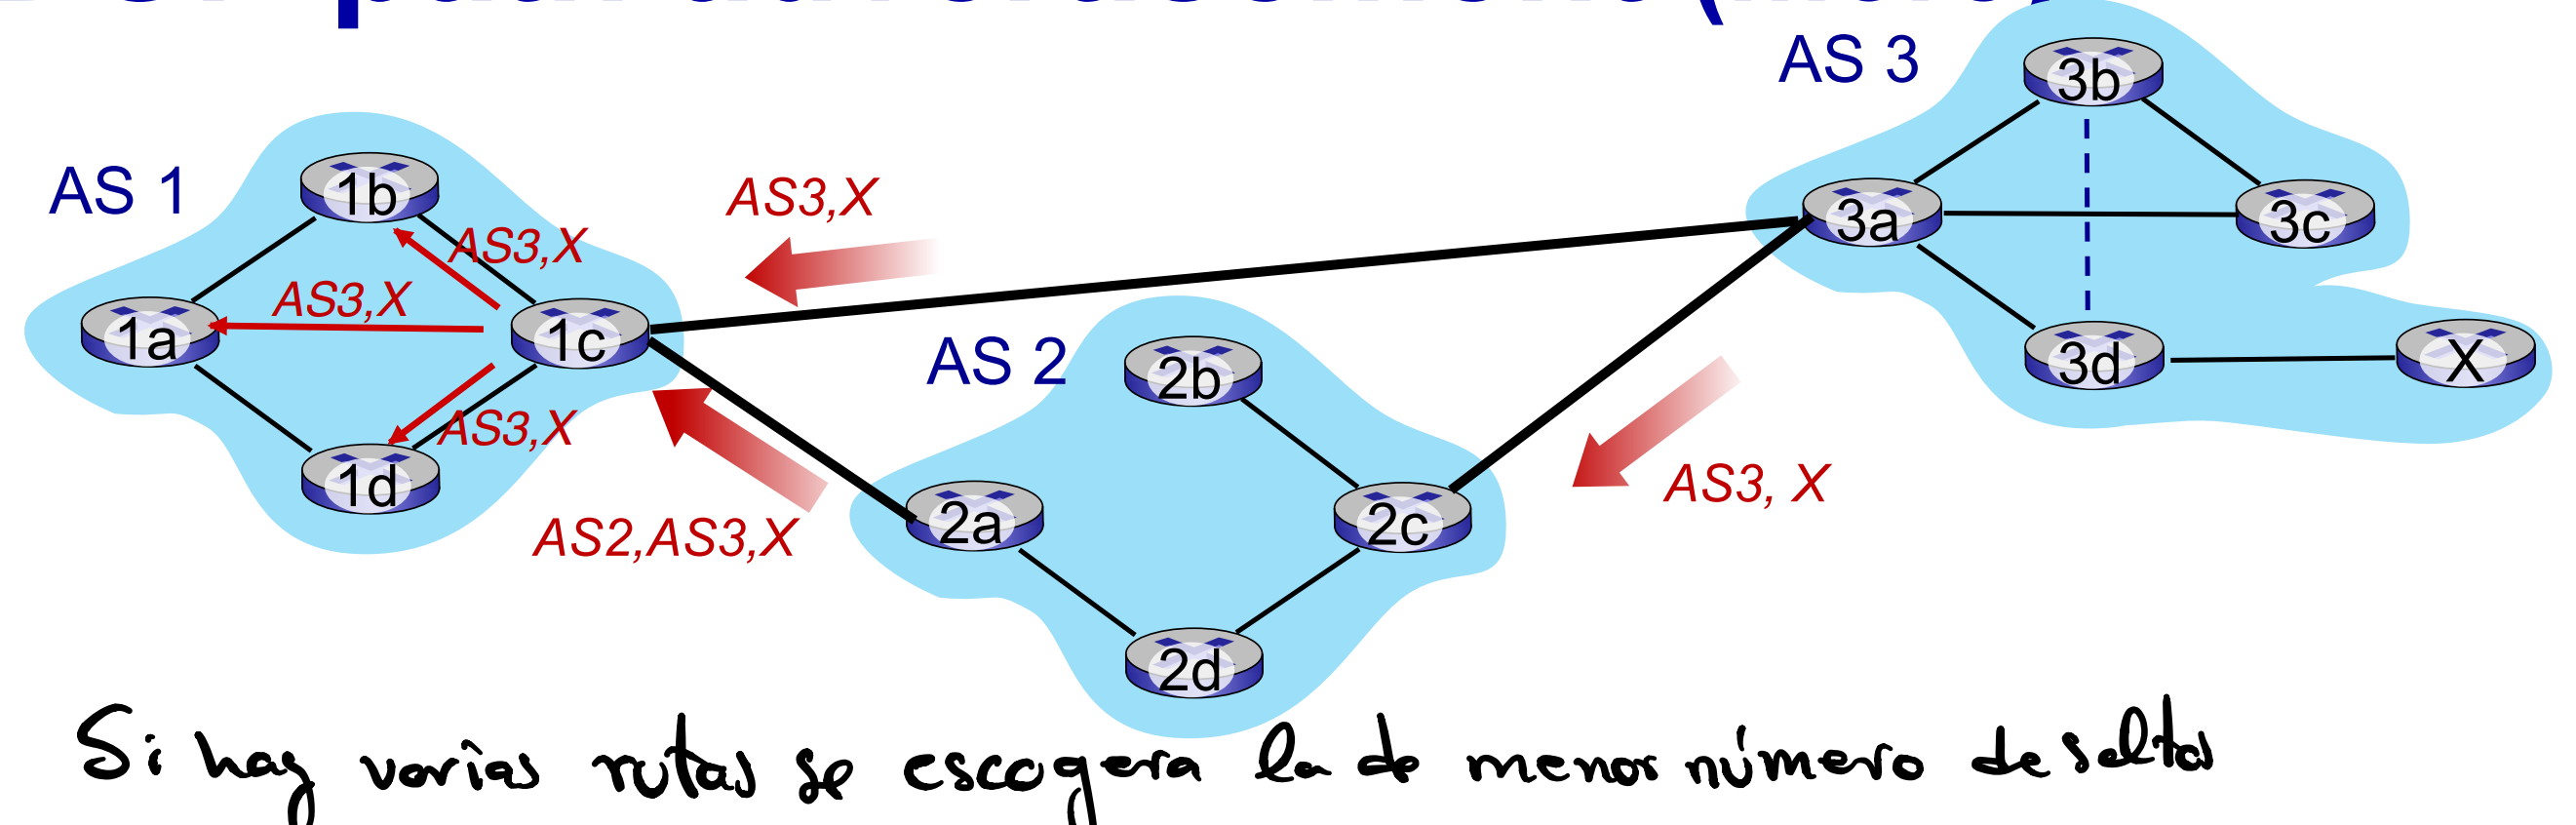
\includegraphics[scale=.15]{Untitled 45.png}}
	\end{figure}
    \item
      Si hay varias rutas se escogerá la de menor número de saltos.
      \end{itemize}
    \end{itemize}
  
\pagebreak
	¿Por qué diferentes enrutados, intra e inter dominio?

    \begin{itemize}
    \item
      Políticas:

      \begin{itemize}
      \item
        Interdominio: el administrador quiere control sobre como enrutar
        su tráfico, y quien enruta a través de su red.
      \item
        Intradominio: administrador único, que busca la eficiencia del
        enrutado, no hace falta negociar al ser solo 1.
      \end{itemize}
    \item
      Escala: Permite reducir el tamaño de tabla y el número de mensajes
      enviados.
    \item
      Rendimiento:

      \begin{itemize}
      \item
        Interdominio: se centra en la política de alcanzar el dominio
        más que en el rendimiento.
      \item
        Intradominio: Se centra en la eficiencia de la ruta.
      \end{itemize}
    \end{itemize}

	Enrutado de la patata caliente -- Hot potato routing: Cuando hay
    varias salidas elige la salida local que conlleva menor coste
    interno. Sin importar si hay más o menos saltos externos al dominio.

	Enrutado broadcast -- por difusión: Envío masivo. Envía paquetes a
    todos los nodos desde el origen. Replicar desde el origen no es
    eficiente. Hay que controlar duplicados.

    \begin{itemize}
    \item
      Inundación: Cuando un nodo recibe un paquete broadcast, envía
      copias a todos sus vecinos.

      \begin{itemize}
      \item
        El problema es que genera ciclos y tormentas de difusión.
      \end{itemize}
    \item
      Inundación controlada: el nodo solo difunde los paquetes broadcast
      si no ha difundido el mismo paquete previamente.

      \begin{itemize}
      \item
        El nodo guarda memoria de la identidad de los paquetes ya
        difundidos
      \item
        O hace Reenvío por el camino inverso -- Reverse path forwarding
        RPF: solo se reenvía un paquete si ha llegado por el camino más
        corto desde su origen, evitando bucles.
      \end{itemize}
	  \pagebreak
    \item
      Árbol de recubrimiento -- Spanning Tree: Ningún nodo recibe
      paquetes redundantes.

      \begin{itemize}
      \item
        Primero, se construye un árbol de nodos.

        \begin{itemize}
        \item
          Método basado en nodo central.

          \begin{itemize}
          \item
            Cada nodo envía un mensaje de adhesión al nodo central,
            origen, por medio de unicast -- unidifusión.
          \item
            Mandan un solo mensaje con destino el origen, si llega se
            establece esa rama del árbol.
          \item
            El mensaje se envía hasta que es recibido por uno que ya
            pertenece al árbol.
          \end{itemize}
        \item
          Los nodos mandan copias solo a lo largo del árbol, a los
          siguientes siguiendo la estructura, excepto al nodo que se lo
          haya enviado.
        \end{itemize}
      \end{itemize}
    \end{itemize}

	Enrutado multicast -- multidifusión, problemas.

    \begin{itemize}
    \item
      Objetivo: Encontrar un árbol que conecte routers que pertenezca al
      grupo multicast.
    \item
      Árbol: no se usan todas las rutas entre routers.
    \item
      Basado en el origen: árboles diferentes para orígenes diferentes.
    \item
      Árbol compartido: mismo árbol para todos los miembros del grupo.
    \end{itemize}

\section{5.6 ICMP: The Internet Control Message Protocol}
\includepdf[pages=-]{docs/s4.6.pdf}

\chapter{TEMA 6: Link Layer}

\section{6.1 Link Layer: Introduction and Services}

    Capa de enlace: Transferencia fiable de tramas entre equipos
    conectados dentro de una misma red de área local. Tiene la
    responsabilidad de transferir datagramas de un nodo al nodo
    físicamente adyacente a través de un enlace.

    Vamos a ver:

    \begin{itemize}
    \item
      Funciones:

      \begin{itemize}
      \item
        Detección y corrección de errores.
      \item
        Compartición de accesos al canal. Regula el acceso.
      \item
        Direccionamiento a nivel MAC.
      \item
        Redes de área local: Ethernet, VLAN.
      \end{itemize}
    \item
      Implementación e instanciación de las tecnologías del nivel de
      enlace.
    \end{itemize}

    Terminología:

    \begin{itemize}
    \item
      Nodos: Hosts y routers.
    \item
      Enlaces: Canales de comunicación que conectan nodos adyacentes.

      \begin{itemize}
      \item
        Wired: cableados.
      \item
        Wireless: inalámbricos.
      \item
        LANs.
      \end{itemize}
    \item
      Trama: Paquete del nivel 2, encapsula datagramas.
    \end{itemize}

    Cada protocolo de enlace proporciona diferentes servicios.

    Los datagramas son transferidos por diferentes protocolos de enlace
    según los distintos enlaces:

    \begin{itemize}
    \item
      Ethernet como primer enlace.
    \item
      Frame delay como enlace intermedio.
    \item
      802.11 como último enlace.
    \end{itemize}

    Servicios de la capa de enlace:

    \begin{itemize}
    \item
      Entramado -- Limitación de tramas:

      \begin{itemize}
      \item
        Encapsula los datagramas dividiéndolos en trozos a los que les
        pone una cabecera, y se identifica el comienzo y fin de cada
        datagrama.
      \item
        Accede al canal si el medio es compartido.
      \item
        Las direcciones MAC identifica origen y destino a nivel de
        enlace, son distintas a la dirección IP.
      \end{itemize}
    \item
      Entrega fiable entre nodos adyacentes:

      \begin{itemize}
      \item
        Rara vez se usan en canales con pocos errores.
      \item
        Enlaces inalámbricos: alta tasa de error.
      \end{itemize}
    \item
      Control de flujo entre nodos: Adecuar la velocidad entre los nodos
      adyacentes origen y destino.
    \item
      Detección de errores: Errores causados por la atenuación de señal,
      ruido. Detecta y avisa al emisor.
    \item
      Corrección de errores: El receptor identifica y corrige errores de
      bit sin necesidad de retransmisión. Técnica: FEQ.
    \item
      Half-duplex y full-duplex: Con half duplex, ambos nodos de los
      extremos del enlace pueden transmitir, pero no a la vez.
    \end{itemize}

    ¿Dónde se implementa?

    \begin{itemize}
    \item
      Está en todos y cada uno de los hosts.
    \item
      Se implementa en el adaptador en NIC -- network interface card
      (Tarjeta de red).
    \item
      Conectado a los buses de los hosts.
    \item
      Combinación de Software, Hardware, Firmware.
      \begin{figure}[H]
        \ffigbox[\FBwidth]
        {\caption{Network Interface Card}}
        {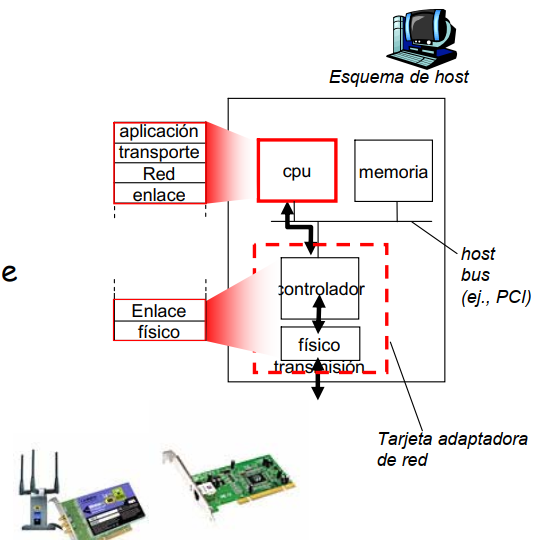
\includegraphics[scale=.3]{Untitled 46.png}}
      \end{figure}
    \end{itemize}

    Comunicación:
    \begin{figure}[H]
      \ffigbox[\FBwidth]
      {\caption{Capa de enlace}}
      {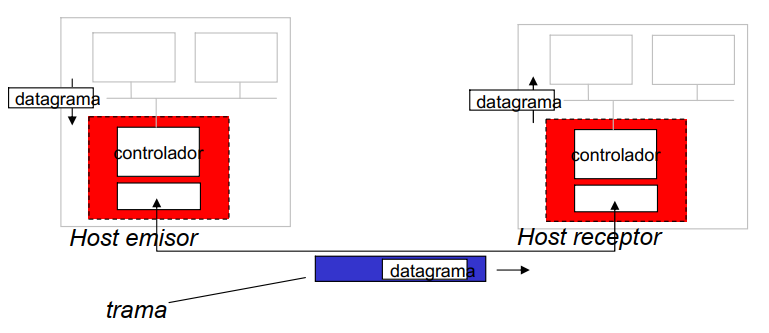
\includegraphics[scale=.35]{Untitled 47.png}}
    \end{figure}
    \begin{itemize}
    \item
      Emisor: Desde la NIC

      \begin{itemize}
      \item
        Encapsula el datagrama en una trama.
      \item
        Añade bits para el control de errores, control de flujo, etc.
      \item
        Mira si el canal está disponible.
      \end{itemize}
    \item
      Se asegura de que está disponible el enlace.
    \item
      Receptor: Lo recibe la NIC.

      \begin{itemize}
      \item
        Busca errores, control de flujo, etc.
      \item
        Extrae el datagrama, y lo pasa a niveles superiores.
      \end{itemize}
    \end{itemize}

    
\section{6.2 Error Detection and Correction Techniques}
\pagebreak
\section{6.3 Multiple Access Protocols}

  
    Dos tipos de enlaces:

    \begin{itemize}
    \item
      Punto a punto: PPP por red telefónica. Enlace punto a punto entre
      conmutador Ethernet y el Host.
    \item
      Difusión -- Broadcast (compartición de cable o medio): Ethernet
      antigua. LAN 802.11 inalámbrica.

      \begin{itemize}
      \item
        Wifi o por satélite.
      \item
        Debe haber mecanismos que controlen quien hace uso del canal.
      \end{itemize}
    \end{itemize}

    Canal único compartido para difusión.

    Interferencia: cuando dos o más nodos transmiten simultáneamente.

    Colisión: Si un nodo recibe dos o más señales a la vez.

    Protocolo de acceso Multiple: Algoritmo distribuido que determina de
    qué modo los nodos comparten el canal. La comunicación sobre como
    compartir el canal va sobre el mismo canal.

    Protocolo de acceso Multiple ideal:

    \begin{itemize}
    \item
      Múltiples accesos al canal con ratio R bps.
    \item
      Deseable:

      \begin{itemize}
      \item
        Cuando 1 nodo quiere transmitir usa velocidad R.
      \item
        Si hay M nodos cada uno usa una fracción R/M.
      \item
        Totalmente descentralizada: No existe un nodo especial para
        coordinar la transmisión. No hay ni turnos ni sincronización de
        relojes.
      \item
        Simple.
      \end{itemize}
    \end{itemize}

    Clasificación:

   \subsection{Reparto del canal -- Partición del canal:}
   Dividir el canal en
      piezas más pequeñas, de tiempo o frecuencias. Reservas un nodo
      para uso exclusivo.
\pagebreak
      \begin{itemize}
      \item
        TDMA: Acceso por multiplexación en el tiempo.

        \begin{itemize}
        \item
          Se accede al canal en rondas.
        \item
          Cada estación tiene espacios de tiempo fijo en cada ronda.
        \item
          Los slots no usados se desaprovechan.
          \begin{figure}[H]
            \ffigbox[\FBwidth]
            {\caption{TDMA}}
            {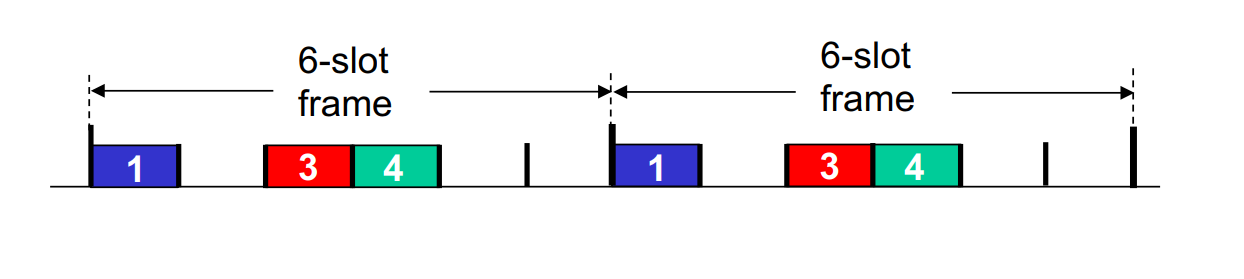
\includegraphics[scale=.25]{Untitled 48.png}}
          \end{figure}
        \end{itemize}
      \item
        FDMA: Acceso múltiple por división en frecuencia.

        \begin{itemize}
        \item
          Se divide la frecuencia entre los accesos.
        \item
          Cada estación tiene su frecuencia fija.
        \item
          El espectro del canal se divide en bandas.
        \item
          Cuando no transmite la banda queda desocupada.
          \begin{figure}[H]
            \ffigbox[\FBwidth]
            {\caption{FDMA}}
            {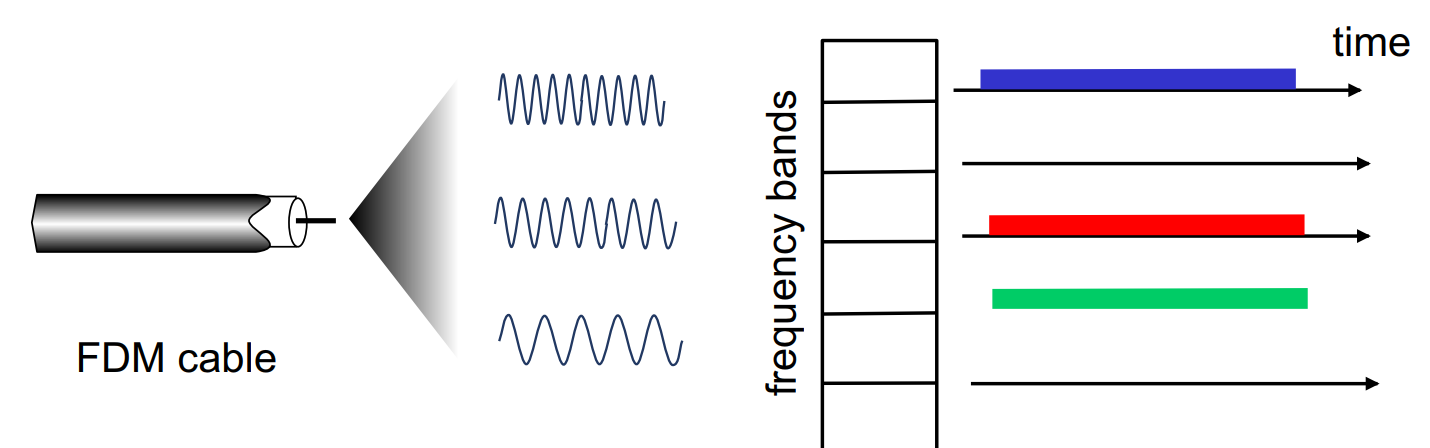
\includegraphics[scale=.2]{Untitled 49.png}}
          \end{figure}
        \end{itemize}
      \end{itemize}

\subsection{Acceso aleatorio -- De contienda} 
No se particiona, permite las
      colisiones y se necesita recuperación de colisiones.

   
        Cuando un nodo tiene un paquete que enviar:

        \begin{itemize}
        \item
          Transmite a la velocidad máxima del canal.
        \item
          No hay coordinación entre nodos.
        \end{itemize}

        Dos o más nodos transmitiendo provocan colisión.

        Especifica:

        \begin{itemize}
        \item
          Como detecta colisiones.
        \item
          Como recuperarse de colisión.
        \end{itemize}
\subsubsection{ALOHA puro -- Pure ALOHA}


          Más simple, no requiere sincronización, si quiere transmite.
        
          Cuando llega la trama, transmite.

          La probabilidad de colisión aumenta: puede colisionar con las
          siguientes.

          Si se produce colisión espera un tiempo aleatorio antes de
          volver intentar transmitir.

          Eficiencia: 18\%, peor que ALOHA ranurado.
          \begin{figure}[H]
            \ffigbox[\FBwidth]
            {\caption{ALOHA puro}}
            {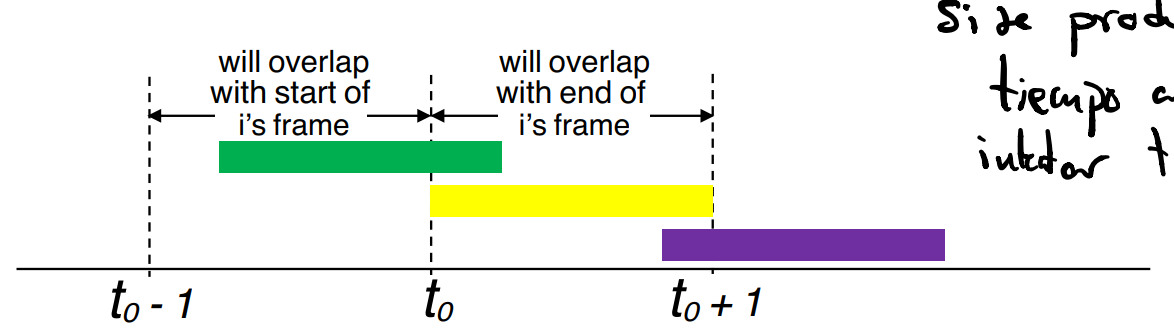
\includegraphics[scale=.25]{Untitled 50.png}}
          \end{figure}

\subsubsection{ALOHA ranurado -- Slotted ALOHA:}

        
        
          Divide el tiempo de uso del canal en ``cuantos''. Cuando hay
          colisión espera un tiempo aleatorio, y cuando pasa el tiempo
          debe esperar que empiece un cuanto/franja.

          Suposiciones:

          \begin{itemize}
          \item
            Tramas del mismo tamaño.
          \item
            Tiempo dividido en franjas del mismo tamaño.
          \item
            Se empieza a transmitir al comienzo del slot.
          \item
            Los nodos se sincronizan.
          \item
            Si dos o más nodos transmiten en el mismo slot, todos los
            demás detectan la colisión.
          \end{itemize}

          Operación:

          \begin{itemize}
          \item
            Cuando un nodo tiene una trama para transmitir:

            \begin{itemize}
              \item
              Si no hay colisión: el nodo puede transmitir una nueva
              trama en el slot siguiente.
            \item
              Si hay colisión: el nodo retransmitirá la trama en cada
              slot subsiguiente con una probabilidad p hasta que
              transmita con éxito. Se espera un tiempo.
            \end{itemize}
          \end{itemize}

          Cuando colisionan ninguna de las transmisiones tiene éxito .

          Pros:

          \begin{itemize}
          \item
            Un nodo activo puede transmitir continuamente a velocidad
            máxima
          \item
            Altamente descentralizado
          \item
            Simple
          \end{itemize}

          Contras:

          \begin{itemize}
          \item
            Colisiones gastan slots
          \item
            Existen slots desocupados
          \item
            Los nodos tienen que ser capaces de detectar colisión en
            menos que transmitir. Puede haber colisiones no detectadas
            por el protocolo.
          \item
            Reloj de sincronización
          \end{itemize}

          Eficiencia: Fracción más larga de slots exitosos.
          \begin{figure}[H]
            \ffigbox[\FBwidth]
            {\caption{Eficiencia ALOHA ranurado}}
            {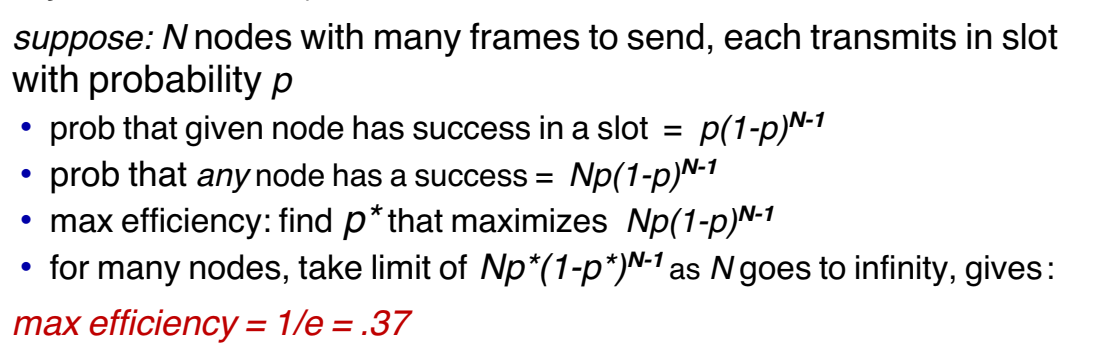
\includegraphics[scale=.25]{Untitled 51.png}}
          \end{figure}
          Como mucho el canal se puede usar para transmisiones con éxito
          el 37\% del tiempo.
          \begin{figure}[H]
            \ffigbox[\FBwidth]
            {\caption{ALOHA ranurado}}
            {\includegraphics[scale=.25]{Untitled 52.png}}
          \end{figure}

\subsubsection{CSMA -- Carrier Sense Multiple Access -- Acceso múltiple con
sondeo de portadora}

        
        
          Escucha el canal, para saber si está libre u ocupada.

          Si está libre transmite, si no espera.

          No interrumpe.

          Mientras transmite no escucha.

          El retraso en la propagación puede hacer que un nodo no oiga a
          otro.

          Colisión: Se malgasta el tiempo en enviar una trama completa.

          A tener en cuenta: El papel que desempeñan la distancia y el
          retraso en la propagación, para determinar la probabilidad de
          colisión.

          CSMA/CD: CSMA con detección de colisiones.

          \begin{itemize}
          \item
            Como CSMA, pero escucha durante la transmisión.
          \item
            Si llega una colisión, este deja de transmitir y espera un
            tiempo aleatorio.
          \item
            Las colisiones se detectan en menos tiempo.
          \item
            Dirección de colisión: Sencillo en LAN cableadas y difícil
            en LAN inalámbricas.
          \end{itemize}

          Uno de los protocolos más usados es Ethernet CSMA/CD:

          \begin{itemize}
          \item
            Recibe de la tarjeta de red el datagrama y crea una trama.
          \item
            Escucha el canal:

            \begin{itemize}
              \item
              Si está libre: Empieza a transmitir.
            \item
              Si está ocupado: Espera que se libere y entonces
              transmite.
            \end{itemize}
          \item
            Si transmite la trama y no hay colisión, se completa.
          \item
            Si detecta otra transmisión, se detiene y manda señal de
            atasco.
          \item
            Después de abortar, NIC entra en retroceso binario (binary
            backoff)

            \begin{itemize}
              \item
              Espera un tiempo y vuelve a escuchar el canal.
            \item
              Mas colisiones provocan que el intervalo de espera se
              alargue de esta manera se ajusta a la carga del canal.
            \item
              Espera 512*K, siendo K un valor entre 0 y \(2^{m}-1\) para
              m colisiones.
            \end{itemize}
          \item
            Mejor rendimiento que ALOHA: más simple, más barato y
            descentralizado.
          \end{itemize}

          CSMA/CA se usa en wifi

          \begin{itemize}
          \item
            El emisor reserva el canal para transmitir tramas, para ello
            transmite pequeños paquetes para solicitar enviar.

            \begin{itemize}
              \item
              El emisor primero transmite RTS -- request to send usando
              CSMA.
            \item
              El receptor envía CTS -- clear to send, los envía la
              estación base en respuesta a RTS, diciendo que emisor
              puede transmitir.
            \item
              Entonces el emisor al que se lo envía transmite y el resto
              los aplaza.
              \begin{figure}[H]
                \ffigbox[\FBwidth]
                {\caption{CSMA/CA}}
                {\includegraphics[scale=.25]{Untitled 53.png}}
              \end{figure}
            \end{itemize}
          \end{itemize}

          Los anteriores son por cables. Ahora por Wireless:

          \begin{itemize}
          \item
            IEEE 802.11: Multiple acceso.

            \begin{itemize}
              \item
              avoid collisions: 2+ nodes transmitting at same time
            \item
              802.11: CSMA - sense before transmitting

              \begin{itemize}
                  \item
                don't collide with detected ongoing transmission by
                another node
              \end{itemize}
            \item
              802.11: no collision detection!

              \begin{itemize}
                  \item
                difficult to sense collisions: high transmitting signal,
                weak received signal due to fading
              \item
                can't sense all collisions in any case: hidden terminal,
                fading
              \item
                goal: avoid collisions: CSMA/CollisionAvoidance
              \end{itemize}
            \end{itemize}
          \item
            IEEE 802.11 MAC Protocol: CSMA/CA

            \begin{itemize}
              \item
              802.11 emisor:

              \begin{itemize}
                  \item
                Si el canal está libre entonces para DIFS

                \begin{itemize}
                      \item
                  entonces transmite la trama.
                \end{itemize}
              \item
                Si está ocupado

                \begin{itemize}
                      \item
                  Empieza un temporizador con tiempo aleatorio.
                \item
                  El contador progresa mientras el canal esta idle.
                \item
                  Cuando para el temporizador transmite.
                \item
                  Si no recibe ACK aumenta el temporizador.
                \end{itemize}
              \end{itemize}
            \item
              802.11 receptor:

              \begin{itemize}
                  \item
                Si llega bien: Espera SIFS y envía ACK.
              \end{itemize}
            \end{itemize}
          \end{itemize}
     

\subsection{Por turnos -- Paso del testigo} Los nodos cogen un turno para su
      uso, y luego ira el del siguiente turno. Sin embargo, si un nodo
      tiene mucho que enviar su turno será más largo.

    
      
        Por división: Comparte el canal eficientemente con alta carga.
        Ineficiente a baja carga.

        Aleatorio: Eficiente a baja carga, un solo nodo puede utilizar
        todo el canal. Con alta carga, hay muchas colisiones.

        Usa lo mejor de ambos.

        Sondeo: El nodo maestro invita a transmitir a los nodos
        esclavos. Se emplea típicamente con nodos tontos.

        \begin{itemize}
        \item
          Hay que tener en cuenta el tiempo que se tarda en sondear, la
          latencia y un único punto de fallo, el nodo maestro.
          \begin{figure}[H]
            \ffigbox[\FBwidth]
            {\caption{Sondeo}}
            {\includegraphics[scale=.25]{Untitled 55.png}}
          \end{figure}
        \end{itemize}
\pagebreak
        Paso de testigo: Una trama especial token es intercambiado de un
        nodo al siguiente.

        \begin{itemize}
        \item
          El token es un mensaje, que cuando un nodo lo tiene pueden
          transmitir y cuando termina se lo pasa a otro.
        \item
          Hay que tener en cuenta el tiempo de pasar el token, la
          latencia y un único punto de fallo, el token.
          \begin{figure}[H]
            \ffigbox[\FBwidth]
            {\caption{Paso de testigo}}
            {\includegraphics[scale=.25]{Untitled 56.png}}
          \end{figure}
        \end{itemize}

\section{6.4 Switched Local Area Networks}

    Direccionamiento a nivel de enlace.

\subsection{Direccionamiento ARP - Address Resolution Protocol}

      \begin{itemize}
      \item
        Direccionamiento MAC

        \begin{itemize}
        \item
          Usado localmente entre interfaces físicamente conectadas.
        \item
          Direcciones de 48 bit, 6 pares de números hexadecimales.

          \begin{itemize}
          \item
            1A-2F-BB-76-09-AD
          \end{itemize}
        \item
          Se reserva la dirección todo 0's y 1's.
        \item
          Cada interfaz tiene una dirección MAC única en esa red de área
          local (se supone que no tiene por qué ser única globalmente,
          pero es muy probable) y una dirección IP local única.
        \item
          IEEE administra la asignación de direcciones MAC.
        \item
          Los fabricantes comprar parte del espacio de direcciones MAC.
        \item
          La dirección MAC es portátil, puede cambiar de LAN, pero la
          jerarquía de dirección IP no es portátil.
        \end{itemize}
      \item
        ARP: Protocolo de Resolución de Direcciones.

        \begin{itemize}
        \item
          Cada nodo IP tiene una tabla de las direcciones MAC
          correspondiente a la IP y un TTL.
          \begin{itemize}
            \item
            \textless{} IP address; MAC address; TTL \textgreater{}
          \end{itemize}
        \item TTL: Tiempo en el que olvidar esa asociación, normalmente 20 minutos.
  Tiempo de vida de una entrada en la tabla.
  \begin{figure}[H]
    \ffigbox[\FBwidth]
    {\caption{Protocolo de Resolución de Direcciones}}
    {\includegraphics[scale=.25]{Untitled 57.png}}
  \end{figure}
        \item Es plug-and-play: Los nodos crean su tabla ARP sin intervención del administrador de red.
        \item Proceso: A quiere enviar un datagrama a B, y la dirección MAC de B no está en la tabla ARP de A.
        \begin{itemize}
         \item A quiere el MAC de B, entonces manda una solicitud de ARP en abierto a todos los nodos.
         \item B recibe la solicitud ARP y responde con su dirección MAC a A.
         \item A recibe la respuesta de B la añade a su ARP table hasta que no sea necesaria, TTL.       
        \end{itemize}
        \item Enviar un datagrama de A a B a través de R:
        \begin{itemize}
          \item Suponemos:
          \begin{itemize}
           \item A conoce la dirección IP y MAC de B.
           \item A conoce la dirección IP y MAC del primer router del primer salto, R 
          \end{itemize}
         
        \item A crea un datagrama IP con la dirección IP origen de A, destino B.
        \item A crea una trama con la dirección MAC de R como destino, la trama contiene el datagrama IP de A a B.
        \item Trama enviada de A a R.
        \item Trama recibida en R, se extrae el datagrama y se pasa a IP. El router lee la trama y datagrama para saber dónde debe ser el siguiente salto.
        \item R reenvía el datagrama con dirección IP origen de A y destino B. No lo cambia
        \item R crea una trama con la dirección MAC de B como destino, la trama contiene el datagrama IP de A a B. Origen R y destino B.
        \item B recibe la trama, extrae el datagrama IP y lo pasa a la capa superior.
        \end{itemize}
        \end{itemize}
      \end{itemize}


  

\subsection{Ethernet}

      Tecnología LAN cableada dominante.

      \begin{itemize}
      \item
        Ampliamente usada.
      \item
        Simple y barato.
      \item
        Velocidad entre 10 Mbps y 400 Gbps.
      \end{itemize}

      Topología física:

      \begin{itemize}
      \item
        La topología en bus fue popular en los 90, todos en el mismo
        dominio de colisión.
      \item
        Hoy en ida se usan switches - conmutadores, que están en el
        centro y tienen hasta capa de enlace 2. Los nodos no colisionan
        con ningún otro.

        \begin{itemize}
        \item
          Cada switch ejecuta el protocolo Ethernet.
        \end{itemize}
      \end{itemize}

      Switch: Donde se conectan los hosts e implementa la lógica de red.

      Router: Separa dominios de difusión.

      Estructura de trama Ethernet:
      \begin{itemize}
        \item El adaptador emisor encapsula IP en una trama Ethernet.
        \begin{figure}[H]
          \ffigbox[\FBwidth]
          {\caption{Estructura de trama Ethernet}}
          {\includegraphics[scale=.25]{Untitled 58.png}}
        \end{figure}
        \pagebreak
        \item Partes:
        \begin{itemize}
         \item Preámbulo: Para sincronizar relojes del dispositivo y separación de tramas.
          \begin{itemize}
           \item 7 bytes con el patrón 10101010 seguido de un byte con el patrón 10101011
         \item se emplea para sincronizar los relojes del emisor y del receptor
          \end{itemize}
          
        \item Direcciones: 6 bytes.
        \item Tipo: Indica el protocolo de nivel de red.
        \item Datos.
        \item CRC: Detección de errores. Se comprueba en la recepción, si se detecta que hay error la trama se descarta.
        \end{itemize}
      
      \end{itemize}
  
  
      Servicio sin conexión, no fiable.

      \begin{itemize}
      \item
        Servicio sin conexión: No existe un protocolo de handshaking -
        negociación entre los NIC emisor y receptor.
      \item
        No fiable: Detecta errores, pero no sabe resolverlos, no envía
        asentimientos. Puede resolver el fallo si se implementa en una
        capa superior transmisión fiable.
      \item
        Protocolo MAC de Ethernet: CSMA/CD no ranurado.
      \end{itemize}
    
      802.3 Estándar Ethernet: Capa enlace y física

      \begin{itemize}
      \item
        Hay diferentes Ethernet según la velocidad y medio de la capa
        física.

        \begin{itemize}
        \item
          El formato de trama y el protocolo MAC son comunes.
        \item
          Velocidad: 2 Mbps, 10 Mbps, 100 Mbps, 1 Gbps, 10 Gbps.
        \item
          Capa física: fibra óptica, cable.
        \end{itemize}
      \end{itemize}

      Redes inalámbricas y móviles:

      \begin{itemize}
      \item
        Hay más dispositivos Wireless que wired (10 a 1 en 2019)
      \item
        Dos importantes retos:

        \begin{itemize}
        \item
          Inalámbrico: Comunicar por enlace Wireless.
        \item
          Movilidad: Manejo del usuario móvil que cambia el punto de
          conexión a la red.
        \end{itemize}
        \pagebreak
      \item
        Elementos:

        \begin{itemize}
        \item
          Hosts inalámbricos: Laptop, smartphone, IoT. Ejecutan
          aplicaciones.
        \item
          Estación base: Típicamente conecta móviles en una red
          cableada.
          \begin{itemize}
      \item
        Relay: Responsable de enviar paquetes entre redes cableadas y
        host cableados.
      \end{itemize}
   
      \item Enlace inalámbrico: Típicamente conecta móviles y la estación base.
            Varios ratios, distintas y frecuencias de transmisión.
            \begin{figure}[H]
              \ffigbox[\FBwidth]
              {\caption{Enlace inalámbricos}}
              {\includegraphics[scale=.25]{Untitled 59.png}}
            \end{figure}
      \item Characteristics of selected wireless links
      \begin{figure}[H]
        \ffigbox[\FBwidth]
        {\caption{haracteristics of selected wireless links}}
        {\includegraphics[scale=.25]{Untitled 60.png}}
      \end{figure}
    \end{itemize}

\item Modo infraestructura:
\begin{itemize}
  \item Handoff: Un móvil puede cambiar de estación base a la que está conectado.
  \item Estación base conecta móviles en una red cableada. 
\end{itemize}
     
\item Modo ad hoc:
\begin{itemize}
  \item No hay estaciones base.
  \item Los nodos se transmiten la información directamente.
  \item Los nodos se organizan ellos mismos, enrutados a través de los mimos.
\end{itemize}
     
\item 802.11 Arquitectura LAN
\begin{itemize}
  \item Los hosts inalámbricos se comunican con la estación base = Access point.
  \item BSS - La infraestructura célula contiene:
  \begin{itemize}
    \item Hosts inalámbricos.
    \item Estación base.
    \item Entre los hosts se usa modo ad hoc.
  \end{itemize}
     
  \item Canales y asociación:
  \begin{itemize}
    \item El espectro se divide en canales con distintas frecuencias.
    \item Los dispositivos que entran se deben asociar con el punto de acceso (Meter la pass del wifi)
    \item Cuando se asocia con un punto de acceso, se puede hacer autenticación, típicamente se hace DHCP para conseguir una IP.
  \end{itemize}
\item Escaneo pasivo:
\begin{figure}[H]
  \ffigbox[\FBwidth]
  {\caption{Escaneo pasivo}}
  {\includegraphics[scale=.25]{Untitled 61.png}}
\end{figure}
  \begin{itemize}
    \item Los beacons frames envían solicitudes para asociarse con los hosts.
    \item Beacon frame: Pequeña trama donde va información sobre el punto de acceso y la MAC.
  \end{itemize}

  \item Escaneo activo:
  \begin{figure}[H]
    \ffigbox[\FBwidth]
    {\caption{Escaneo activo}}
    {\includegraphics[scale=.2]{Untitled 62.png}}
  \end{figure}
  \begin{itemize}
    \item Los dispositivos son los que van mandando solicitudes.
  \end{itemize}

  \item Trama: Direccionamiento.
  \begin{figure}[H]
    \ffigbox[\FBwidth]
    {\caption{Trama: Direccionamiento}}
    {\includegraphics[scale=.2]{Untitled 63.png}}
  \end{figure}
  \begin{itemize}
    \item Partes:
    \begin{itemize}
      \item Dentro de control de trama:
      
      Tipo: Tipo de trama, RTS, CTS, ACK y data.

      \item Duración: Duración de reserva del tiempo de transmisión. RTS petición y CTS envía.
      \item Dirección 1: Dirección MAC de destino.
      \item Dirección 2: Dirección MAC del que transmite la trama.
      \item Dirección 3: Dirección MAC del router asociado al Access point.
      \item Seq control – secuencia de control: Detección de tramas. Para saber cuál es.
      \item Dirección 4: Dirección MAC cuando se usa modo ad hoc.
    \end{itemize}
  
  \end{itemize}



    \end{itemize}
  \end{itemize}

  \subsection{Switches}

  Un switch es un dispositivo en la capa de enlace con una función
  importante.

  \begin{itemize}
    \item
      Almacena y reenvía tramas ethernet.
    \item
      Cuando recibe una trama mira la dirección MAC y con la tabla
      sabe por qué enlace lo debe pasar, usando CSMA/CD.
    \item
      Es transparente para los hosts.
    \item
      plug-and-play, self-learning: Autoaprenden, no hace falta
      configurarlo según se reciben tramas se van rellenando las
      tablas de manera dinámica. Cada nodo tiene una tabla de reenvío
      donde guarda la dirección MAC, la interfaz un TTL.
  \end{itemize}

  Los hosts se conectan a los switches con conexiones dedicadas
  directamente.

  El protocolo ethernet se usa en cada enlace de entrada:

  \begin{itemize}
    \item
      Sin colisiones y puedo full duplex.
    \item
      Cada enlace es un dominio de colisión.
    \item
      Un switch puede recibir y reenviar datos simultáneamente, pero
      por un mismo enlace solo se puede transmitir uno a la vez.
  \end{itemize}

  Autoaprende: El switch aprende cuáles son los hosts alcanzables
  según la MAC origen e interfaces de entrada de las tramas que
  recibe.

    \begin{itemize}
      \item
        Se va rellenando la tabla con el uso del switch.
      \item
        Si recibe por la interfaz una trama que procede de A, sabe que
        si algo es para A se enviara por esa interfaz.
      \item
        Si no lo conoce inunda las interfaces.
      \item
        Proceso:

      \begin{enumerate}
        \item
          Registra enlace y MAC del emisor.
        \item
          Indexa la tabla usando la dirección de destino.
        \item
          Si tiene la entrada para ese destino.

          \begin{enumerate}
            \item
              Si la interfaz es la misma de la que viene la descarta.
            \item
              Si no lo envía por la interfaz correspondiente.
          \end{enumerate}
        \item
          Si no la conoce, inunda las interfaces, excepto por la que
          viene.
      \end{enumerate}
    \end{itemize}

  Los switches que autoaprenden pueden conectarse, cuando se ha
  reenviado por los que pasa se conectan al almacenar las entradas.
  Switch vs router:

  \begin{itemize}
    \item
      Ambas almacenan y reenvían los datos que reciben, unos tramas
      otros datagramas.

      \begin{itemize}
        \item
          router: De la capa de red.
        \item
          switch: De la capa de enlace.
      \end{itemize}
    \item
      Ambos usan tablas:

      \begin{itemize}
        \item
          router: Se basa en IP.
        \item
          switch: Se basa en MAC.
      \end{itemize}
  \end{itemize}
  \pagebreak
\subsection{VLAN - Redes de Area Local Virtual}

  

      Un solo dominio de broadcast, todo el tráfico debe cruzar la LAN
      entera.

      Permite que dispositivos conectados a un switch pertenezcan a otra
      red de área local.

      Permite a un usuario que no está conectado físicamente, pertenecer
      lógicamente a la red mediante un switch.

      VLAN basado en el puerto:

      \begin{itemize}
      \item
        Según el puerto configurado está en una red u otra.
      \item
        1 switch muchas VLAN.
      \item
        Aislamiento de tráfico: Hace que las tramas no se expandan, ni
        colisionen, entre VLAN distintas solo se popula en la VLAN.
      \item
        Pertenencia dinámica: La pertenencia a la VLAN es dinámica al
        cambiar puerto.
      \item
        Reenvió entre VLAN: Mediante enrutamiento. En la práctica se
        vende la combinación de router y switch.
      \item
        En 802.1Q hay 12 bits para el ID de la VLAN
      \item
        Puerto trunk: Para intercambiar tramas entre dispositivos de una
        VLAN, pero que físicamente están en varios switches.
        \begin{itemize}
          \item Las tramas en VLAN en varios switches no pueden ser el standard
          802.1 
          \item Se usan 802.1Q para añadir en la cabecera o quitar la
          cabecera entre los puertos trunk.
          \begin{figure}[H]
            \ffigbox[\FBwidth]
            {\caption{Formato trama VLAN}}
            {\includegraphics[scale=.25]{Untitled 63.png}}
          \end{figure}
        \end{itemize}
      \end{itemize}
 

\subsection{MPLS}


        Solución tecnológica para multiplexar el tráfico, entre la capa
        2 y 3.

        Su objetivo es conseguir reenvío IP de alta velocidad entre
        redes de router capaces de MPLS, de esta tecnología.

        Se consulta más rápido usando el identificador.

        Coge ideas de redes de circuitos, pero con datagramas IP. Con
        respecto a que se pone un identificador dependiendo del origen y
        fin.

        Añade una cabecera entre la cabecera ethernet y el datagrama.

        Reenvía solo consultando la cabecera MPLS, no mira el resto, usa
        sus propias tablas.

        Prioriza las rutas de baja latencia.

        Flexible: El reenvío puede ser distinto que el de IP, ya que
        prioriza baja latencia.

        Permite detectar rápidamente fallos.

        A diferencia de IP, la ruta se puede basar tanto en la dirección
        de origen como la de destino, no solo en la de destino.

        Como lo hace:
        \begin{itemize}
      \item Va modificando las tablas de enrutamiento de otras capas.
      \item Los routers MPLS usan RSVP-TE para configurar el reenvío, que es una
        modificación de OSPF, un protocolo de estado de enlace por
        inundación.
        \begin{figure}[H]
          \ffigbox[\FBwidth]
          {\caption{MPLS}}
          {\includegraphics[scale=.25]{Untitled 66.png}}
        \end{figure}
    \end{itemize}

\section{6.7 A Day in the Life of a Web Page Request}

\section{7.1 Introduction}

\section{7.3 WiFi: 802.11 Wireless LANs}

\includepdf[pages=-]{docs/s5.1.pdf}

\includepdf[pages=-]{docs/s5.2.pdf}

\includepdf[pages=-]{docs/s5.3.pdf}


\part{Laboratorios}
\chapter{Practica DNS}
\includepdf[pages=-]{docs/PRACTICA_-_DNS.pdf}

\chapter{Practica de Direccionamiento}
\includepdf[pages=-]{docs/understandIP.pdf}

\chapter{Practica de routers}
\includepdf[pages=-]{docs/manual_linksys_uc3m.pdf}
\includepdf[pages=-]{docs/4_routers_eng_VM_con_instrucciones.pdf}


\end{document}